\documentclass[12pt,a4paper]{report}

% ═══════════════════════════════════════════════════════════════════
% PACKAGES ET CONFIGURATION TYPOGRAPHIQUE
% ═══════════════════════════════════════════════════════════════════
\usepackage[utf8]{inputenc}
\usepackage[T1]{fontenc}
\usepackage[french]{babel}
\usepackage{geometry}
\usepackage{graphicx}
\usepackage{float}
\usepackage{array}
\usepackage{longtable}
\usepackage{booktabs}
\usepackage{hyperref}
\usepackage{xcolor}
\usepackage{setspace}
\usepackage{titlesec}
\usepackage{fancyhdr}
\usepackage{amsmath,amssymb}
\usepackage{subcaption}
\usepackage{tikz}
\usepackage{enumitem}

\geometry{left=2.5cm,right=2.5cm,top=2.5cm,bottom=2.5cm}
\onehalfspacing

\setlength{\headheight}{15pt}
\addtolength{\topmargin}{-3pt}

\hypersetup{
    colorlinks=true,
    linkcolor=blue,
    urlcolor=blue,
    citecolor=blue
}

\pagestyle{fancy}
\fancyhf{}
\fancyhead[L]{Chatbot Intelligent d'Analyse RSE \& Audit ESG}
\fancyhead[R]{\thepage}

\titleformat{\chapter}[display]
{\normalfont\bfseries\Large}
{\chaptername\ \thechapter}
{10pt}
{\Huge}

\begin{document}

% ═══════════════════════════════════════════════════════════════════
% PAGE DE GARDE OFFICIELLE
% ═══════════════════════════════════════════════════════════════════
\begin{titlepage}
    \centering
    {\scshape\Large République Tunisienne\\
    Ministère de l'Enseignement Supérieur et de la Recherche Scientifique\\[0.5cm]
    \textbf{ÉCOLE NATIONALE D'INGÉNIEURS}\\[1.5cm]}

    {\Huge \textbf{Rapport de Projet de Fin d'Études}\\}
    {\Large Pour l'obtention du Diplôme National d'Ingénieur en Informatique\\}
    {\large Spécialité : Génie Logiciel \& Intelligence Artificielle\\[1.2cm]}

    \rule{\linewidth}{0.6mm}\\[0.4cm]
    {\LARGE \textbf{Conception et Réalisation d'un Chatbot Intelligent Multi-Modèles pour l'Analyse Automatisée des Rapports RSE et l'Audit de Conformité ESG}\\}
    \rule{\linewidth}{0.6mm}\\[0.6cm]

    {\large \textit{Architecture hybride combinant Vision par Ordinateur (CNN Custom), Transformers (CamemBERT), Reconnaissance d'Entités (spaCy NER), Recherche Vectorielle (ChromaDB), LLM Local (Mistral 7B) et Moteur d'Audit Réglementaire Hybride}}

    \vfill

    \begin{minipage}{0.48\textwidth}
        \begin{flushleft} \large
            \textbf{Réalisé par :}\\
            Azer \textsc{Ben Rejeb}
        \end{flushleft}
    \end{minipage}
    \begin{minipage}{0.48\textwidth}
        \begin{flushright} \large
            \textbf{Organisme d'accueil :}\\
            \textbf{RSE Time}\\
            \vspace{0.2cm}
            \textbf{Encadrant Entreprise :}\\
            Équipe Data \& RSE Time\\
            \vspace{0.2cm}
            \textbf{Encadrant Académique :}\\
            Tuteur Universitaire
        \end{flushright}
    \end{minipage}

    \vfill
    {\large Année Universitaire 2025 -- 2026}
\end{titlepage}

\pagenumbering{roman}

% ═══════════════════════════════════════════════════════════════════
% DÉDICACES & REMERCIEMENTS
% ═══════════════════════════════════════════════════════════════════
\chapter*{Dédicaces}
\addcontentsline{toc}{chapter}{Dédicaces}

À mes très chers parents, pour leurs sacrifices inestimables, leur affection indéfectible et leur soutien continu qui ont guidé mes pas vers l'accomplissement de mes études d'ingénieur.\\

À mes frères et sœurs, pour leur tendresse, leurs encouragements constants et les moments précieux partagés.\\

À l'ensemble de mes professeurs et encadrants académiques, qui ont su transmettre la rigueur scientifique, l'éthique professionnelle et la passion de l'intelligence artificielle.\\

À tous mes collègues et amis, avec qui j'ai partagé des années inoubliables d'apprentissage, d'efforts et de réussite.

\newpage

\chapter*{Remerciements}
\addcontentsline{toc}{chapter}{Remerciements}

Ce travail de fin d'études n'aurait pu voir le jour sans l'appui et l'engagement de nombreuses personnes envers qui j'exprime ma plus sincère reconnaissance.\\

Je tiens tout d'abord à remercier chaleureusement la direction et l'ensemble des collaborateurs de l'entreprise \textbf{RSE Time} pour m'avoir accueilli en tant que stagiaire ingénieur au sein de leurs équipes. L'autonomie accordée, les échanges stimulants avec les experts en durabilité et les ressources mises à ma disposition ont constitué un cadre d'apprentissage exceptionnel.\\

J'adresse ma vive gratitude à mes encadrants professionnels et académiques pour leur suivi régulier, leurs orientations méthodologiques précises et leurs précieux conseils tout au long de la conduite de ce projet.\\

Mes sincères remerciements vont également aux membres du jury qui ont accepté d'examiner ce rapport et d'évaluer ce travail d'ingénierie.

\newpage

% ═══════════════════════════════════════════════════════════════════
% RÉSUMÉ & ABSTRACT
% ═══════════════════════════════════════════════════════════════════
\chapter*{Résumé}
\addcontentsline{toc}{chapter}{Résumé}

L'évaluation de la performance extra-financière et sociétale des entreprises est devenue une obligation stratégique majeure sous l'impulsion des cadres réglementaires internationaux (standards universels de la \textit{Global Reporting Initiative} -- GRI Standards 2021, directive européenne sur le reporting de durabilité des entreprises -- CSRD, et normes européennes ESRS). Cependant, les rapports annuels de Responsabilité Sociétale des Entreprises (RSE) et les Déclarations de Performance Extra-Financière (DPEF) représentent des documents extrêmement volumineux (dépassant fréquemment 150 pages), visuellement denses et sémantiquement complexes. Leur audit manuel requiert en moyenne plusieurs jours par rapport et expose les auditeurs à des risques critiques d'omission d'indicateurs de conformité.\\

Pour surmonter ces verrous, ce Projet de Fin d'Études présente la conception, l'implémentation et la validation expérimentale d'un système d'aide à la décision complet, multi-modèles et hautement sécurisé, développé selon la démarche méthodologique industrielle \textbf{CRISP-DM} (\textit{Cross-Industry Standard Process for Data Mining}).\\

Les contributions majeures de ce travail d'ingénieur s'articulent autour des axes suivants :
\begin{enumerate}
    \item \textbf{Vision par Ordinateur (CNN) :} Conception d'un Réseau de Neurones Convolutif dédié, doté d'une fonction de \textbf{scoring continu softmax} ($0.0 \rightarrow 1.0$), évaluant la densité informative de chaque page PDF sans suppression destructrice d'information ;
    \item \textbf{Constitution d'un Gold-Standard d'Apprentissage :} Réalisation d'une \textbf{annotation manuelle intégrale et experte de 3\,872 paragraphes} issus de 33 rapports d'entreprises internationales, équilibrés entre les piliers Environnemental (1\,639), Social (1\,260) et Gouvernance (973) ;
    \item \textbf{Benchmark de Modélisation NLP :} Progression scientifique démontrée entre une approche Baseline (89,33\,\%), un modèle d'ensemble Random Forest (90,71\,\%) et un modèle Transformer CamemBERT fine-tuné atteignant \textbf{90,88\,\% d'accuracy} et \textbf{90,84\,\% de F1-macro} ;
    \item \textbf{Reconnaissance d'Entités Nommées (spaCy NER) :} Entraînement d'un pipeline d'extraction automatique des indicateurs clés (valeurs numériques, unités physiques, années, indicateurs GRI) avec un \textbf{F1-score de 95,97\,\%} ;
    \item \textbf{Architecture RAG Sécurisée sur Site :} Indexation sémantique dans la base vectorielle ChromaDB couplée au grand modèle de langue local Mistral 7B (via Ollama), garantissant la confidentialité des données et l'absence d'hallucinations grâce à la traçabilité intégrale des sources documentaires ;
    \item \textbf{Moteur d'Audit Réglementaire Hybride :} Synergie novatrice combinant règles déterministes par expressions régulières et \textbf{filet de sécurité sémantique par similarité d'embeddings}, permettant un gain net de \textbf{+25,0\,\% de détection} sur les indicateurs obligatoires GRI.
\end{enumerate}

Le système est industrialisé sous forme d'une architecture micro-services animée par une API REST FastAPI et interfacée via un tableau de bord décisionnel Streamlit offrant la génération automatique de synthèses d'audit en PDF.\\

\textbf{Mots-clés :} RSE, ESG, Méthodologie CRISP-DM, Vision par Ordinateur (CNN), CamemBERT, spaCy NER, RAG, ChromaDB, Mistral 7B, GRI Standards, CSRD, FastAPI, Streamlit.

\newpage

\chapter*{Abstract}
\addcontentsline{toc}{chapter}{Abstract}

Evaluating corporate extra-financial and sustainability performance has become a critical strategic obligation driven by international regulatory frameworks (Global Reporting Initiative -- GRI Standards 2021, EU Corporate Sustainability Reporting Directive -- CSRD, and European Sustainability Reporting Standards -- ESRS). However, corporate CSR (Corporate Social Responsibility) reports and non-financial statements are voluminous documents (routinely exceeding 150 pages), characterized by high visual density and heterogeneous layouts. Manual assessment is time-consuming (averaging multiple business days per report) and carries substantial risks of overlooking mandatory regulatory disclosures.\\

To address these operational bottlenecks, this graduation project presents the design, engineering, and empirical validation of an end-to-end, multi-model, and privacy-preserving decision-support system, developed rigorously following the \textbf{CRISP-DM} (\textit{Cross-Industry Standard Process for Data Mining}) methodology.\\

The key engineering and scientific contributions of this work include:
\begin{enumerate}
    \item \textbf{Computer Vision (CNN):} A custom Convolutional Neural Network operating with continuous softmax probability scoring ($0.0 \rightarrow 1.0$), evaluating page ESG density while eliminating the catastrophic risk of silent data loss;
    \item \textbf{Curated Gold-Standard Benchmark Dataset:} An \textbf{exhaustive manual expert annotation of 3,872 paragraphs} extracted from 33 real-world multi-sector CSR reports, balanced across Environmental (1,639), Social (1,260), and Governance (973) pillars;
    \item \textbf{Comparative NLP Classification Benchmark:} Progression from a TF-IDF Baseline (89.33\%), to an optimized Random Forest (90.71\%), up to a fine-tuned CamemBERT Transformer achieving \textbf{90.88\% accuracy} and a \textbf{90.84\% macro F1-score};
    \item \textbf{Custom Named Entity Recognition (spaCy NER):} Automated extraction of physical quantities, measurement units, reporting years, and GRI indicator references with an exceptional \textbf{95.97\% F1-score};
    \item \textbf{On-Premise Grounded RAG Pipeline:} High-performance vector retrieval via ChromaDB paired with the Mistral 7B open-source LLM executed locally via Ollama, ensuring zero corporate data leakage and hallucination-free generation with page citations;
    \item \textbf{Hybrid Compliance Auditing Engine:} A hybrid architecture coupling deterministic regular expressions with a \textbf{semantic embedding safety net}, yielding a verified \textbf{+25.0\% increase in regulatory disclosure retrieval} over 12 essential GRI indicators.
\end{enumerate}

The complete pipeline is deployed as a production-ready micro-services architecture powered by a FastAPI REST backend and delivered to sustainability consultants through an interactive Streamlit dashboard featuring automated PDF audit report generation.\\

\textbf{Keywords:} CSR, ESG, CRISP-DM Methodology, Computer Vision (CNN), CamemBERT, spaCy NER, RAG, ChromaDB, Mistral 7B, GRI Standards, CSRD, FastAPI, Streamlit.

\newpage

% ═══════════════════════════════════════════════════════════════════
% TABLES DES MATIÈRES, FIGURES ET TABLEAUX
% ═══════════════════════════════════════════════════════════════════
\tableofcontents
\newpage
\listoffigures
\newpage
\listoftables
\newpage

% ═══════════════════════════════════════════════════════════════════
% LISTE DES ABRÉVIATIONS ET ACRONYMES
% ═══════════════════════════════════════════════════════════════════
\chapter*{Liste des abréviations et acronymes}
\addcontentsline{toc}{chapter}{Liste des abréviations et acronymes}

\begin{longtable}{p{3.2cm}p{11.5cm}}
\toprule
\textbf{Acronyme} & \textbf{Définition complète} \\
\midrule
\endfirsthead
\toprule
\textbf{Acronyme} & \textbf{Définition complète} \\
\midrule
\endhead
\bottomrule
\endfoot

\textbf{API} & \textit{Application Programming Interface} (Interface de programmation) \\
\textbf{BERT} & \textit{Bidirectional Encoder Representations from Transformers} \\
\textbf{CamemBERT} & Modèle Transformer pré-entraîné sur le corpus français OSCAR \\
\textbf{CNN} & \textit{Convolutional Neural Network} (Réseau de Neurones Convolutif) \\
\textbf{CRISP-DM} & \textit{Cross-Industry Standard Process for Data Mining} \\
\textbf{CSR} & \textit{Corporate Social Responsibility} (Responsabilité Sociétale des Entreprises) \\
\textbf{CSRD} & \textit{Corporate Sustainability Reporting Directive} (Directive UE 2022/2464) \\
\textbf{DPEF} & Déclaration de Performance Extra-Financière \\
\textbf{EFRAG} & \textit{European Financial Reporting Advisory Group} \\
\textbf{ESG} & Environnemental, Social et Gouvernance \\
\textbf{ESRS} & \textit{European Sustainability Reporting Standards} \\
\textbf{FastAPI} & Framework web Python moderne, asynchrone et hautement performant \\
\textbf{GES / GHG} & Gaz à Effet de Serre / \textit{Greenhouse Gases} \\
\textbf{GPU} & \textit{Graphics Processing Unit} \\
\textbf{GRI} & \textit{Global Reporting Initiative} \\
\textbf{IA / AI} & Intelligence Artificielle / \textit{Artificial Intelligence} \\
\textbf{JSON} & \textit{JavaScript Object Notation} \\
\textbf{KPI} & \textit{Key Performance Indicator} (Indicateur Clé de Performance) \\
\textbf{LLM} & \textit{Large Language Model} (Grand Modèle de Langage) \\
\textbf{NER} & \textit{Named Entity Recognition} (Reconnaissance d'Entités Nommées) \\
\textbf{NLP} & \textit{Natural Language Processing} (Traitement Automatique du Langage Naturel) \\
\textbf{OCR} & \textit{Optical Character Recognition} (Reconnaissance Optique de Caractères) \\
\textbf{PDF} & \textit{Portable Document Format} \\
\textbf{PFE} & Projet de Fin d'Études \\
\textbf{RAG} & \textit{Retrieval-Augmented Generation} (Génération Augmentée par Récupération) \\
\textbf{REST} & \textit{Representational State Transfer} \\
\textbf{RF} & \textit{Random Forest} (Forêt d'Arbres Décisionnels Aléatoires) \\
\textbf{RSE} & Responsabilité Sociétale des Entreprises \\
\textbf{SBTi} & \textit{Science Based Targets initiative} \\
\textbf{TF-IDF} & \textit{Term Frequency - Inverse Document Frequency} \\
\textbf{UML} & \textit{Unified Modeling Language} \\
\textbf{UI / UX} & \textit{User Interface / User Experience} \\
\bottomrule
\end{longtable}

\newpage
\pagenumbering{arabic}

% ═══════════════════════════════════════════════════════════════════
% CHAPITRE 1 : CONTEXTE GÉNÉRAL ET DÉMARCHE CRISP-DM
% ═══════════════════════════════════════════════════════════════════
\chapter{Contexte général, organisme d'accueil et méthodologie CRISP-DM}

\section{Introduction}
L'intégration des critères Environnementaux, Sociaux et de Gouvernance (ESG) au cœur de la stratégie d'entreprise représente l'une des mutations économiques et réglementaires les plus profondes de cette décennie. Jadis facultative ou cantonnée à des exercices de communication institutionnelle, la publication annuelle d'un rapport de durabilité est désormais strictement encadrée par des textes législatifs internationaux d'une grande rigueur. Les entreprises doivent justifier avec précision de leur trajectoire de décarbonation, de la sécurité de leurs collaborateurs, de la mixité de leurs instances dirigeantes et de leurs pratiques éthiques.\\

Cependant, ces rapports annuels RSE -- combinant Déclarations de Performance Extra-Financière (DPEF), bilans carbone conformes au protocole GHG et index de conformité GRI -- comptent régulièrement entre 150 et 350 pages. Pour les cabinets d'audit, les analystes d'investissement durable et les directions RSE, l'exploitation manuelle de cette masse documentaire colossale est devenue un goulot d'étranglement majeur. C'est dans ce contexte stimulant que s'inscrit ce Projet de Fin d'Études mené au sein de l'entreprise \textbf{RSE Time}.

\section{Présentation de l'organisme d'accueil : RSE Time}

\subsection{Identité, mission et domaines d'expertise}
Fondée par des experts de la transition environnementale et des technologies logicielles, \textbf{RSE Time} est une entreprise innovante spécialisée dans le conseil en développement durable et le déploiement de solutions numériques d'évaluation extra-financière. Sa mission première consiste à accélérer la transition écologique des organisations en automatisant la collecte, le contrôle de conformité et la modélisation de leurs indicateurs d'impact.\\

L'offre de valeur de RSE Time s'articule autour de trois piliers complémentaires :
\begin{itemize}
    \item \textbf{L'audit de conformité réglementaire :} Évaluation de la conformité des rapports d'entreprises aux référentiels internationaux (GRI Standards, directive européenne CSRD, recommandations TCFD) ;
    \item \textbf{La stratégie bas-carbone et matérialité :} Calcul et trajectoire des bilans d'émissions de gaz à effet de serre (Scopes 1, 2 et 3) et modélisation de la double matérialité selon les normes ESRS ;
    \item \textbf{Le développement d'outils numériques intelligents :} Conception d'applications analytiques facilitant l'accès direct aux données RSE pour les directions générales, les auditeurs internes et les investisseurs.
\end{itemize}

\begin{figure}[H]
    \centering
    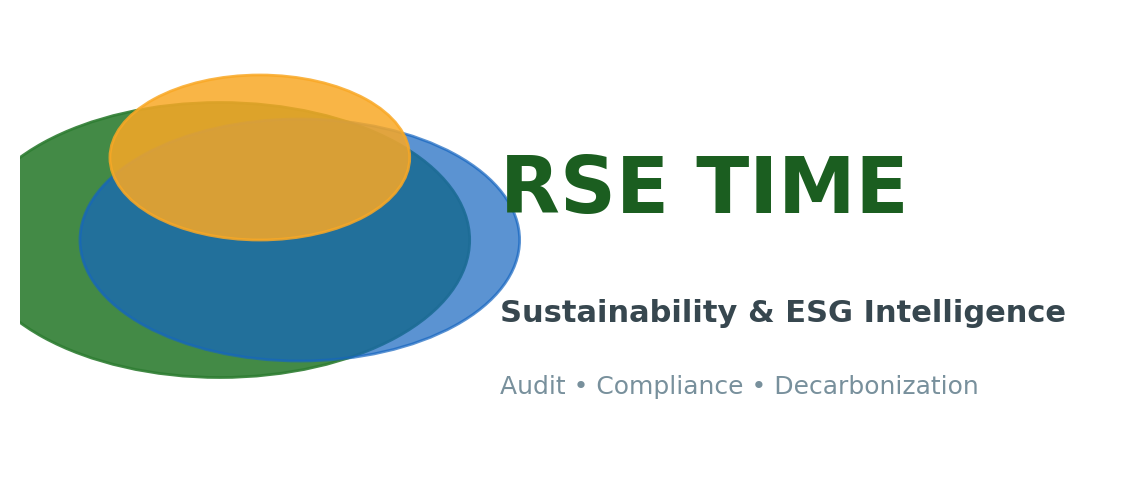
\includegraphics[width=0.65\textwidth]{figures/fig_rse_time_logo.png}
    \caption{Identité visuelle officielle de l'organisme d'accueil RSE Time}
    \label{fig:logo_rse_time}
\end{figure}

\subsection{Organisation interne et positionnement du projet PFE}
L'entreprise RSE Time est organisée en pôles complémentaires favorisant la synergie entre consultants métier et ingénieurs en technologies avancées. Comme le met en évidence l'organigramme de la figure~\ref{fig:organigramme}, ce projet de fin d'études a été accueilli au sein du \textbf{Pôle IA \& Data Science}. L'ingénieur stagiaire a ainsi travaillé en étroite collaboration avec les analystes seniors du Pôle Conseil RSE et l'équipe Architecture Logicielle, garantissant une parfaite adéquation entre rigueur technologique et besoins concrets du terrain.

\begin{figure}[H]
    \centering
    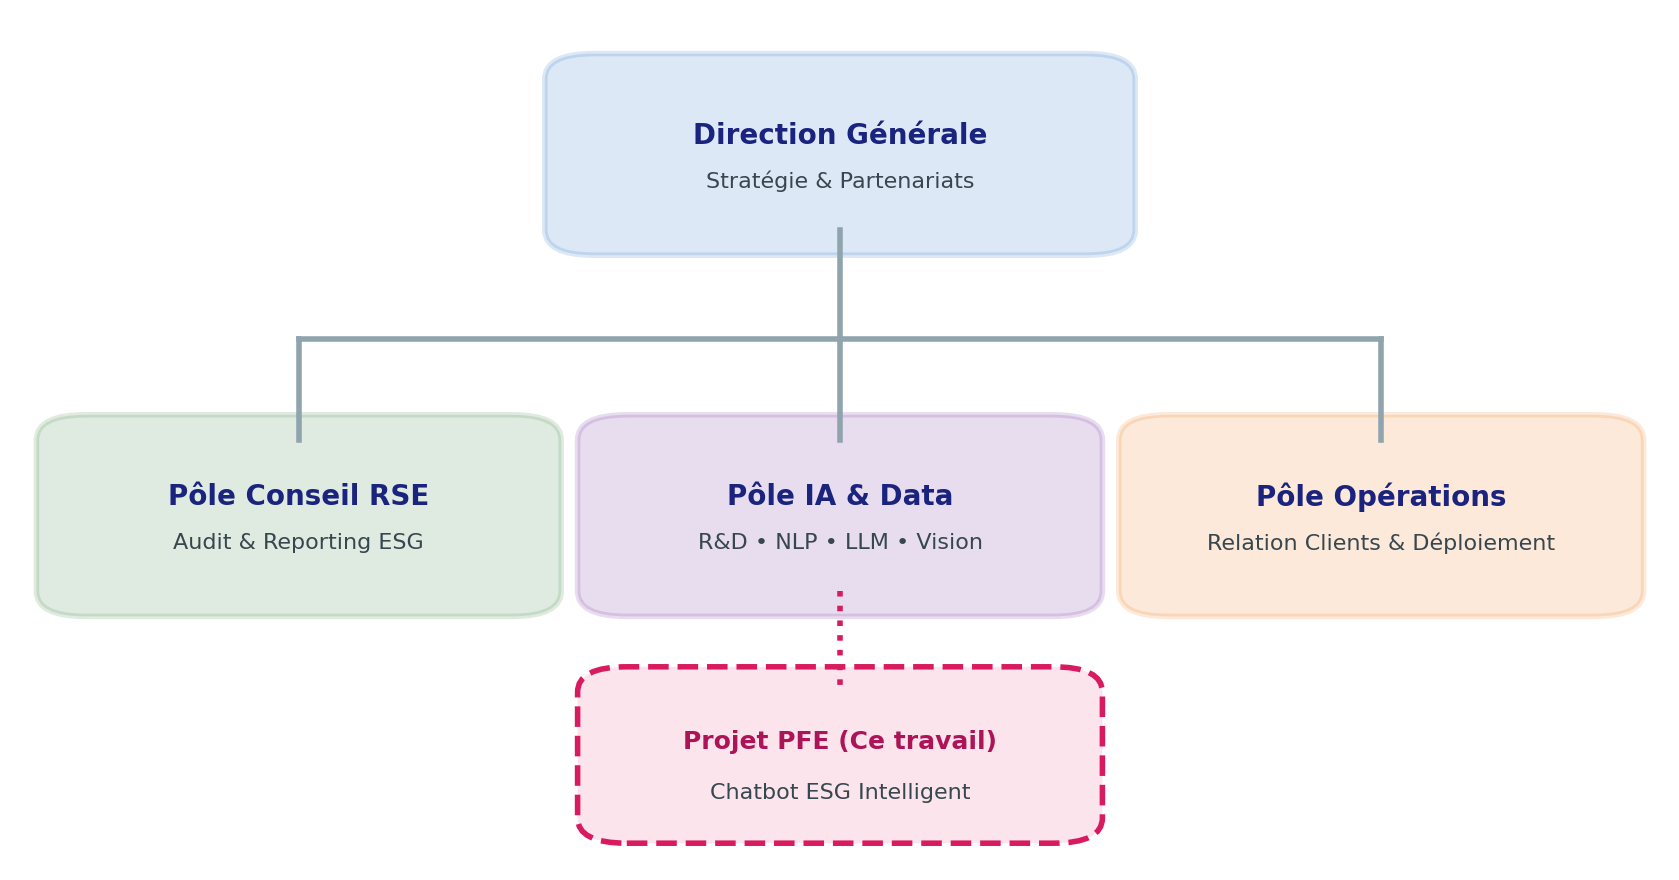
\includegraphics[width=0.92\textwidth]{figures/fig_organigramme_rse_time.png}
    \caption{Structure organisationnelle de RSE Time et insertion du projet PFE}
    \label{fig:organigramme}
\end{figure}

\section{Étude de l'existant et analyse critique}
Face au défi du traitement des rapports RSE, plusieurs approches ont été explorées sur le marché et dans les cabinets de conseil :
\begin{enumerate}
    \item \textbf{L'audit manuel traditionnel :} Réalisé par des consultants juniors via des feuilles de calcul et des recherches textuelles de mots-clés sous un lecteur PDF. Cette méthode est extrêmement coûteuse (entre 3 et 5 jours de travail par document d'envergure) et hautement sujette à la fatigue cognitive, entraînant l'omission fréquente d'indicateurs dissimulés dans des notes annexes ;
    \item \textbf{Les plateformes SaaS généralistes de gestion ESG :} (Exemples : Greenly, Sweep, EcoVadis). Bien qu'efficaces pour la saisie directe de données par l'entreprise déclarante, ces plateformes sont démunies face à un rapport PDF volumineux externe déjà rédigé. Elles ne permettent pas d'interroger directement le texte ou de vérifier l'exactitude des calculs présentés ;
    \item \textbf{L'utilisation directe de LLMs publics en mode « boîte noire » :} L'interrogation de modèles fermés (tels que GPT-4 ou Claude via des API externes) pose des problèmes rédhibitoires : risques critiques de fuite d'informations financières stratégiques avant publication, limitations strictes sur la fenêtre de contexte ne permettant pas d'ingérer 200 pages sans tronquature, et \textbf{phénomène d'hallucination}, un modèle génératif brut pouvant inventer des chiffres d'émissions avec une grande assurance apparente.
\end{enumerate}

Le tableau~\ref{tab:comparaison_existant} dresse une analyse comparative des différentes approches face aux exigences industrielles de RSE Time.

\begin{table}[H]
    \centering
    \begin{tabular}{|p{3.8cm}|p{2.6cm}|p{2.6cm}|p{3.2cm}|p{2.8cm}|}
        \hline
        \textbf{Critères d'évaluation} & \textbf{Audit manuel} & \textbf{Plateformes ESG} & \textbf{LLM Public cloud} & \textbf{Notre solution} \\
        \hline
        \textbf{Temps d'analyse} & 3 à 5 jours & Variable & Quelques minutes & \textbf{< 1 minute} \\
        \hline
        \textbf{Confidentialité / Local} & Oui & Non (Cloud) & Non (Fuite cloud) & \textbf{Oui (100\% local)} \\
        \hline
        \textbf{Absence d'hallucination} & Oui & Sans objet & Non (Risque fort) & \textbf{Oui (Ancrage RAG)} \\
        \hline
        \textbf{Traçabilité des pages} & Manuelle & Aucune & Très approximative & \textbf{Exacte (Page/Chunk)} \\
        \hline
        \textbf{Contrôle GRI formel} & Long et fastidieux & Partiel & Aléatoire & \textbf{Hybride (Regex + Sém.)} \\
        \hline
    \end{tabular}
    \caption{Tableau comparatif de l'existant face aux exigences d'ingénierie}
    \label{tab:comparaison_existant}
\end{table}

\section{Problématique et objectifs du projet}

\subsection{Problématique}
L'exploitation des rapports RSE au sein de RSE Time et de ses entreprises clientes soulève une triple problématique :
\begin{itemize}
    \item \textbf{La volumétrie et l'hétérogénéité des documents :} Comment traiter de façon fluide des fichiers PDF volumineux mêlant tableaux imbriqués, graphiques infographiques, colonnes journalistiques et blocs de texte narratifs ?
    \item \textbf{La fiabilité absolue requise par la réglementation :} Comment offrir une interface de dialogue en langage naturel avec la base documentaire qui garantisse l'intégrité factuelle des réponses et cite systématiquement le numéro de page source de la preuve ?
    \item \textbf{La détection exhaustive des conformités GRI Standards :} Comment automatiser le diagnostic de conformité lorsque les indicateurs obligatoires sont formulés avec des vocabulaires imprévus qui échappent aux simples recherches par mots-clés ?
\end{itemize}

\subsection{Objectifs scientifiques et techniques}
Pour répondre rigoureusement à cette problématique, les objectifs majeurs assignés à ce travail d'ingénieur sont :
\begin{enumerate}
    \item Concevoir un composant de \textbf{Vision par Ordinateur (CNN)} chargé d'évaluer la densité ESG de chaque page sans perte destructive d'information via un scoring continu softmax ;
    \item Constituer et annoter de manière experte un \textbf{corpus de référence de 3\,872 paragraphes} équilibrés sur les piliers Environnemental, Social et Gouvernance ;
    \item Mener une étude comparative expérimentale rigoureuse entre trois architectures NLP (Baseline, Random Forest et Transformer CamemBERT) ;
    \item Développer un modèle sur-mesure de \textbf{Reconnaissance d'Entités Nommées (spaCy NER)} pour isoler les métriques quantitatives, leurs unités et les codes réglementaires ;
    \item Construire un pipeline de \textbf{Génération Augmentée par Récupération (RAG)} associant la base vectorielle ChromaDB au LLM open-source Mistral 7B déployé localement ;
    \item Développer un \textbf{moteur d'audit réglementaire hybride} associant règles syntaxiques et filet de sécurité sémantique pour combler les manques de formulation ;
    \item Déployer l'ensemble au travers d'une architecture micro-services FastAPI et d'un tableau de bord décisionnel Streamlit.
\end{enumerate}

\section{Méthodologie de conduite de projet : CRISP-DM}

\subsection{Justification du choix méthodologique}
La gestion d'un projet d'ingénierie intégrant plusieurs briques avancées d'Intelligence Artificielle (Deep Learning en Vision, modèles de Transformers, bases vectorielles et Grands Modèles de Langage) ne saurait être menée selon un cycle en cascade rigide (\textit{Waterfall}). Les projets d'IA imposent en effet des rétroactions constantes entre l'exploration de la donnée, l'ingénierie des caractéristiques et l'optimisation des hyperparamètres.\\

Comme l'atteste l'étude empirique résumée dans la figure~\ref{fig:methodologies}, le standard international \textbf{CRISP-DM} (\textit{Cross-Industry Standard Process for Data Mining}) représente la méthodologie la plus adoptée dans le secteur de la Data Science et de l'IA appliquée (plébiscitée par 44\,\% des directeurs techniques et chefs de projet, surpassant Scrum et les approches agiles conventionnelles). Sa nature cyclique, sa focalisation sur la compréhension des données métier et la formalisation claire de ses livrables en font le cadre idéal pour ce travail de fin d'études.

\begin{figure}[H]
    \centering
    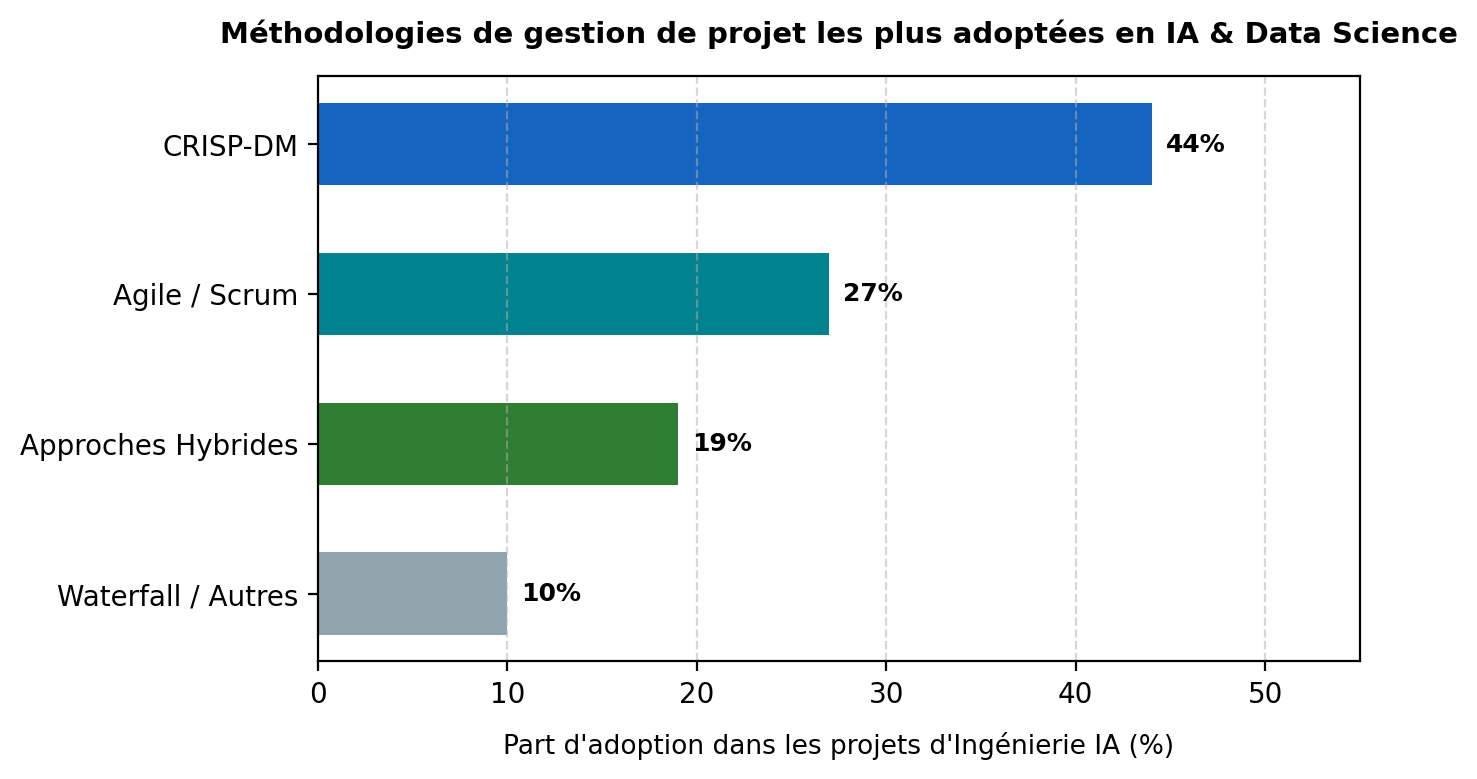
\includegraphics[width=0.75\textwidth]{figures/fig_methodologies_ia.png}
    \caption{Taux d'adoption des méthodologies de gestion de projet en Intelligence Artificielle}
    \label{fig:methodologies}
\end{figure}

\subsection{Déclinaison des six phases CRISP-DM sur le projet Chatbot ESG}
Le cycle de vie CRISP-DM repose sur six étapes interdépendantes et itératives, schématisées dans la figure~\ref{fig:crisp_dm} :

\begin{figure}[H]
    \centering
    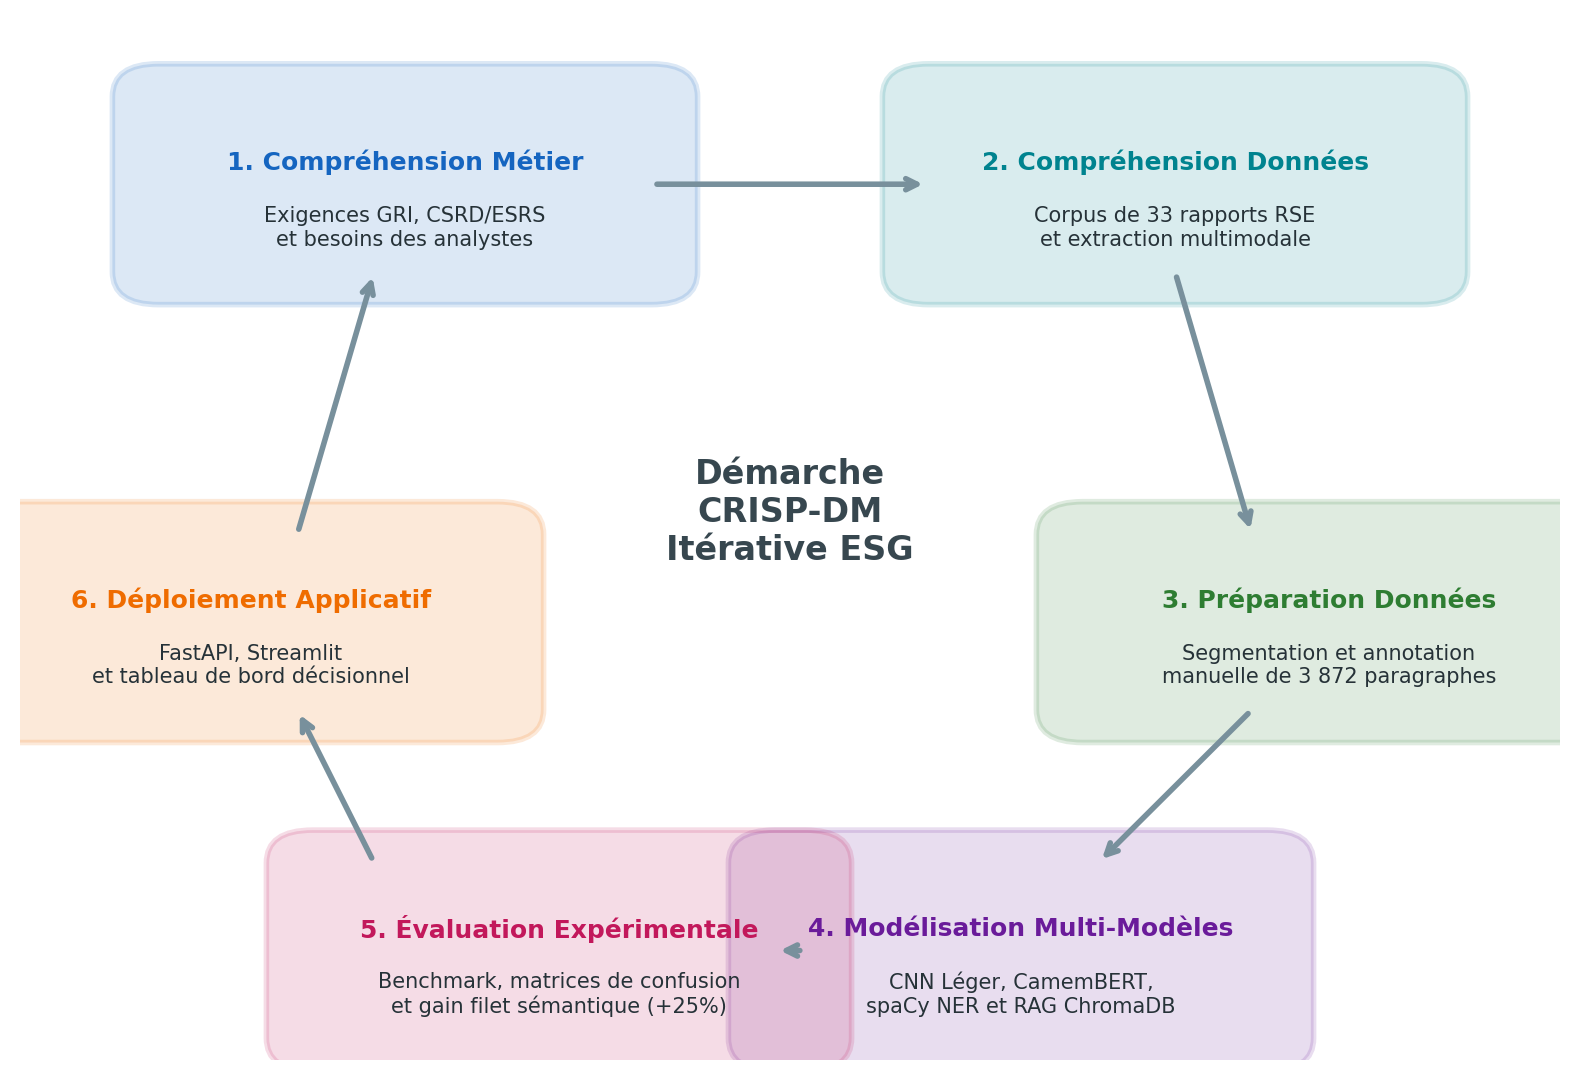
\includegraphics[width=0.85\textwidth]{figures/fig_crisp_dm.png}
    \caption{Cycle itératif de la méthodologie CRISP-DM appliqué au projet Chatbot ESG}
    \label{fig:crisp_dm}
\end{figure}

\begin{enumerate}[label=\textbf{Phase \arabic* :}, wide=0pt]
    \item \textbf{Compréhension Métier (\textit{Business Understanding}) :}\\
    Immersion auprès des analystes de RSE Time pour appréhender les impératifs de l'audit extra-financier. Analyse approfondie des standards GRI (GRI 302 pour l'énergie, GRI 305 pour les émissions, GRI 401 pour l'emploi, etc.) et des exigences émergentes de la directive CSRD. Définition des indicateurs clés de succès (KPIs) : temps de réponse inférieur à 2 secondes, zéro hallucination, et rappel élevé sur les divulgations réglementaires ;
    
    \item \textbf{Compréhension des Données (\textit{Data Understanding}) :}\\
    Collecte d'un corpus industriel de 33 rapports RSE internationaux au format PDF (représentant plus de 3\,500 pages de données réelles). Analyse de l'hétérogénéité des formats de mise en page, du ratio texte/image et identification des défis d'extraction (tableaux scannés, césures lexicales, bruit visuel) ;
    
    \item \textbf{Préparation des Données (\textit{Data Preparation}) :}\\
    Conception du pipeline d'ingestion multimodale (extraction vectorielle native \texttt{pdfplumber} couplée à un moteur OCR \texttt{EasyOCR} de secours). Normalisation textuelle, suppression des en-têtes/pieds de page répétitifs et segmentation en paragraphes cohérents (80 à 900 caractères). Réalisation d'une \textbf{annotation manuelle experte intégrale de 3\,872 paragraphes} labellisés selon les critères d'évaluation GRI ;
    
    \item \textbf{Modélisation (\textit{Modeling}) :}\\
    Conception et entraînement successif des modules d'apprentissage automatique :
    \begin{itemize}
        \item Réseau Convolutif (CNN) pour le calcul de la probabilité continue de pertinence de chaque page ;
        \item Entraînement et benchmark de trois architectures de classification NLP (Baseline TF-IDF, Random Forest et Transformer CamemBERT) ;
        \item Modèle spaCy NER entraîné sur des motifs spécifiques d'audit ;
        \item Pipeline RAG articulant les représentations vectorielles d'all-MiniLM-L6-v2 stockées sous ChromaDB et la génération contrôlée par Mistral 7B ;
        \item Filet sémantique d'audit basé sur la similarité cosinus ;
    \end{itemize}
    
    \item \textbf{Évaluation (\textit{Evaluation}) :}\\
    Validation rigoureuse des modèles sur un banc de test indépendant de 581 paragraphes. Évaluation par matrices de confusion, F1-scores macro, temps de latence à l'inférence et mesure quantitative du gain de couverture réglementaire (+25,0\,\% d'indicateurs récupérés) ;
    
    \item \textbf{Déploiement (\textit{Deployment}) :}\\
    Architecture logicielle micro-services : backend REST FastAPI haute performance, persistance SQLite de l'historique conversationnel, et dashboard interactif Streamlit avec génération automatisée de synthèses d'audit au format PDF.
\end{enumerate}

\subsection{Tableau synoptique de cadrage du projet}
Le tableau~\ref{tab:cadrage_crisp} résume de façon synthétique la structure de conduite du projet, en reliant objectifs, tâches d'ingénierie et livrables concrets pour chacune des phases CRISP-DM.

\begin{table}[H]
    \centering
    \begin{tabular}{|p{3.2cm}|p{3.8cm}|p{4.5cm}|p{3.3cm}|}
        \hline
        \textbf{Phase CRISP-DM} & \textbf{Objectifs visés} & \textbf{Tâches d'ingénierie} & \textbf{Livrables concrets} \\
        \hline
        \textbf{1. Compréhension Métier} & Cadrer les exigences réglementaires et les besoins des auditeurs & Analyse détaillée GRI 2021 \& CSRD, entretiens avec experts RSE, définition des KPIs & Cahier des charges et spécifications fonctionnelles \\
        \hline
        \textbf{2. Compréhension Données} & Caractériser les documents réels et évaluer la faisabilité & Collecte de 33 rapports PDF, audit typographique et structurel & Corpus brut de 3\,500+ pages \\
        \hline
        \textbf{3. Préparation Données} & Construire le jeu de données d'apprentissage de référence & Ingestion multimodale OCR, segmentation et annotation manuelle rigoureuse & Dataset expert de 3\,872 paragraphes E/S/G \\
        \hline
        \textbf{4. Modélisation} & Entraîner et optimiser les cinq briques d'IA & Entraînement CNN, benchmark de 3 classifieurs NLP, spaCy NER, ChromaDB/Mistral & Poids et pipelines des modèles optimisés \\
        \hline
        \textbf{5. Évaluation} & Valider scientifiquement les performances & Test set indépendant ($n=581$), matrices de confusion, calibration seuil & Rapports de validation et 15 graphiques d'analyse \\
        \hline
        \textbf{6. Déploiement} & Rendre le système opérationnel pour les utilisateurs & Backend REST FastAPI, interface décisionnelle Streamlit, export PDF & Application complète opérationnelle \\
        \hline
    \end{tabular}
    \caption{Cadrage exhaustif des phases, tâches et livrables de la méthodologie CRISP-DM}
    \label{tab:cadrage_crisp}
\end{table}

\section{Planification prévisionnelle du projet et gestion des risques}

\subsection{Diagramme de Gantt du projet}
Le projet a été structuré sur une période de 24 semaines (correspondant aux six mois de stage d'ingénieur). La figure~\ref{fig:gantt_crisp_dm} présente le diagramme de Gantt détaillant l'enchaînement temporel des phases CRISP-DM, ainsi que le positionnement des quatre jalons clés de validation (\textit{Milestones}) :
\begin{itemize}
    \item \textbf{Jalon 1 (Semaine 4) :} Cadrage réglementaire et spécifications fonctionnelles validés ;
    \item \textbf{Jalon 2 (Semaine 12) :} Pipeline d'ingestion opérationnel et corpus de 3\,872 paragraphes intégralement annoté ;
    \item \textbf{Jalon 3 (Semaine 19) :} Modèles de vision, classification NLP (CamemBERT), NER et RAG entraînés et validés sur banc d'essai ;
    \item \textbf{Jalon 4 (Semaine 24) :} Déploiement de l'API FastAPI, finalisation du dashboard Streamlit et livraison finale de la solution.
\end{itemize}

\begin{figure}[H]
    \centering
    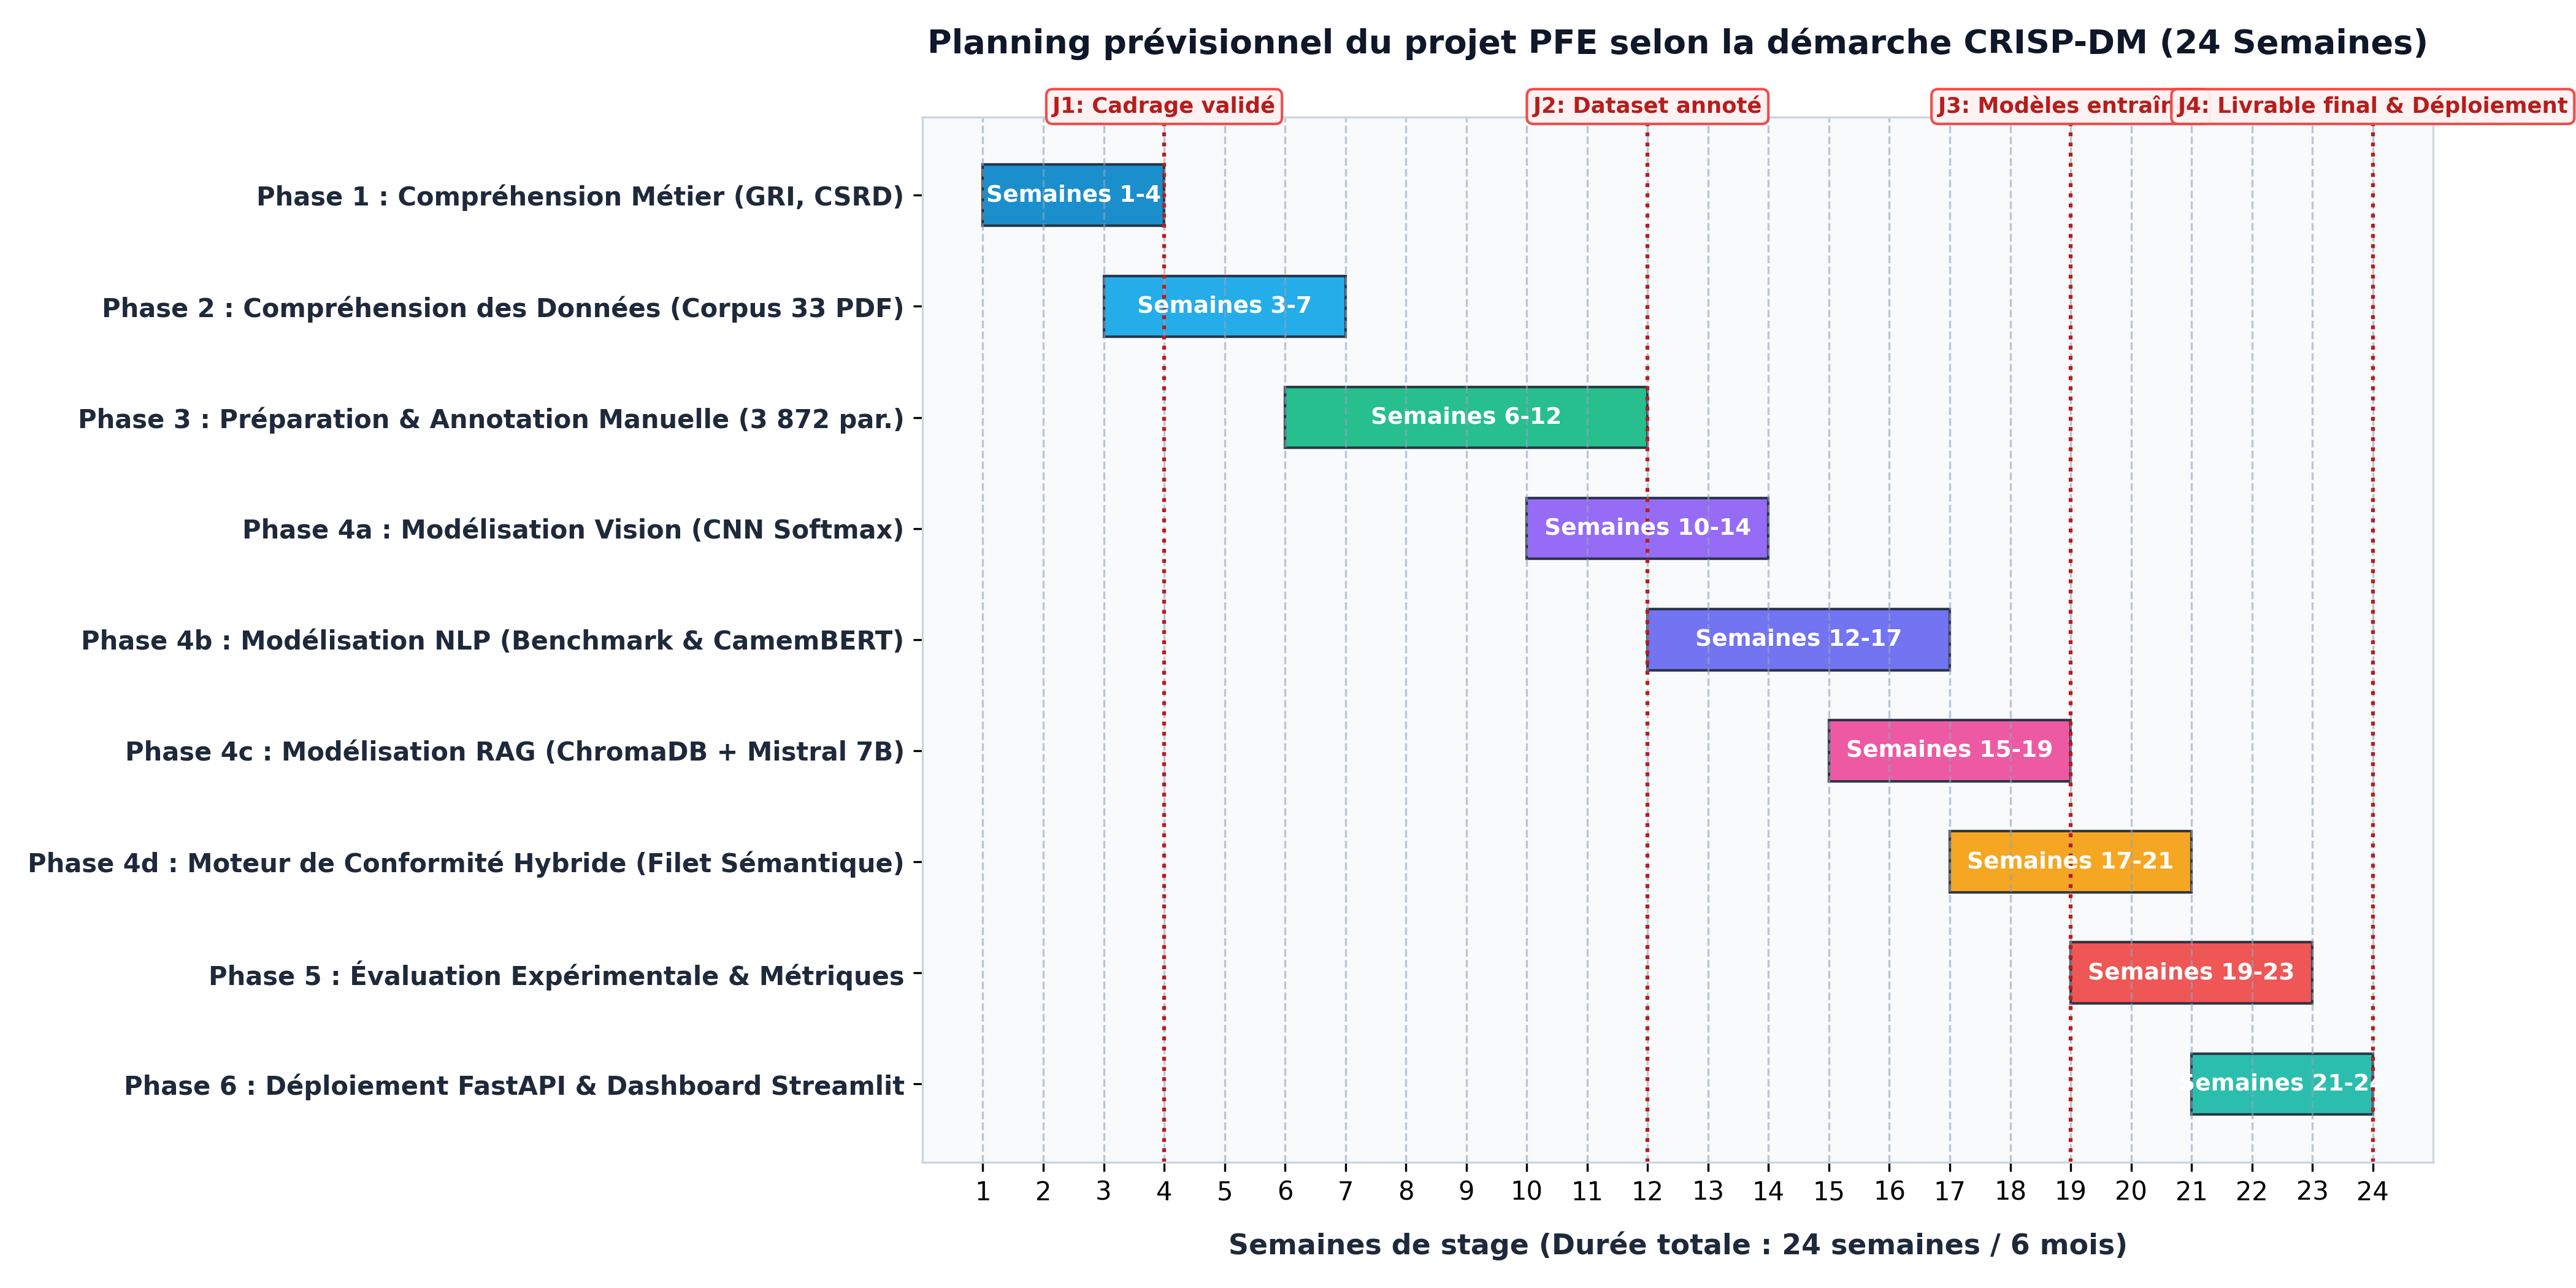
\includegraphics[width=0.98\textwidth]{figures/fig_gantt_crisp_dm.png}
    \caption{Planning prévisionnel du projet PFE selon la démarche CRISP-DM (24 Semaines)}
    \label{fig:gantt_crisp_dm}
\end{figure}

\subsection{Matrice des risques et plan de mitigation}
Tout projet d'Intelligence Artificielle comporte des incertitudes inhérentes à la qualité des données et à la complexité des modèles. Le tableau~\ref{tab:matrice_risques} récapitule les principaux risques identifiés et les stratégies de mitigation mises en place.

\begin{table}[H]
    \centering
    \begin{tabular}{|p{3.5cm}|p{2cm}|p{2cm}|p{6.8cm}|}
        \hline
        \textbf{Risque identifié} & \textbf{Probabilité} & \textbf{Impact} & \textbf{Plan de mitigation appliqué} \\
        \hline
        Perte d'informations dans les pages peu denses & Moyenne & Critique & Remplacement du filtrage rigide par seuil binaire par un scoring continu softmax ($0.0 \rightarrow 1.0$) préservant 100\% des pages \\
        \hline
        Biais d'annotation du corpus d'apprentissage & Faible & Élevé & Protocole d'annotation experte manuelle avec grille formelle GRI et double contrôle de cohérence \\
        \hline
        Hallucinations du LLM sur les chiffres clés & Forte & Critique & Architecture RAG stricte avec injection de contexte limité et citation obligatoire de la page source \\
        \hline
        Fuite de données d'entreprises confidentielles & Moyenne & Critique & Choix exclusif de modèles open-source souverains (Mistral 7B, CamemBERT) déployés sur site \\
        \hline
        Variations terminologiques des indicateurs GRI & Forte & Élevé & Implémentation du filet de sécurité sémantique par similarité cosinus sur les embeddings \\
        \hline
    \end{tabular}
    \caption{Matrice d'évaluation des risques et stratégies de mitigation}
    \label{tab:matrice_risques}
\end{table}

\section{Conclusion du chapitre}
Ce premier chapitre a posé les fondations organisationnelles et méthodologiques du projet. L'accueil au sein de RSE Time a permis de cibler une problématique d'audit bien réelle. L'adoption rigoureuse du cadre international CRISP-DM garantit une démarche d'ingénierie itérative, centrée sur la donnée et résolument tournée vers un produit livrable à fort impact opérationnel. Le chapitre suivant s'attachera à poser les fondements théoriques et l'état de l'art technologique nécessaires à la réalisation de notre système.

\newpage

% ═══════════════════════════════════════════════════════════════════
% CHAPITRE 2 : ÉTAT DE L'ART ET FONDEMENTS THÉORIQUES
% ═══════════════════════════════════════════════════════════════════
\chapter{Fondements théoriques et écosystème technologique}

\section{Introduction}
La réalisation d'un système décisionnel capable d'analyser des rapports d'entreprises requiert la convergence de trois grands domaines de l'informatique moderne : la réglementation internationale extra-financière, le Traitement Automatique du Langage Naturel (NLP) et la Vision par Ordinateur. Ce chapitre explore les fondements théoriques, les modèles mathématiques sous-jacents et l'écosystème technologique mobilisés pour bâtir notre solution.

\section{Cadre réglementaire : Les standards GRI 2021 et la directive CSRD}

\subsection{Les standards universels et thématiques de la GRI}
Créée sous l'égide du Programme des Nations Unies pour l'Environnement (PNUE), la \textbf{Global Reporting Initiative} (GRI) est le référentiel le plus largement adopté dans le monde pour la reddition de comptes sur le développement durable. Sa révision majeure de 2021 clarifie les exigences selon une taxonomie hiérarchique :
\begin{itemize}
    \item \textbf{GRI 100 (Standards Universels) :} Fondements du reporting (GRI 1), divulgations générales sur l'organisation (GRI 2) et gestion des thèmes matériels prioritaires (GRI 3) ;
    \item \textbf{GRI 200 (Standards Économiques et de Gouvernance) :} Intégrité des affaires, lutte contre la corruption (GRI 205), comportement anti-concurrentiel (GRI 206) et politique fiscale ;
    \item \textbf{GRI 300 (Standards Environnementaux) :} Gestion de l'énergie (GRI 302), prélèvements et rejets d'eau (GRI 303), émissions directes et indirectes de GES (GRI 305), gestion des déchets et économie circulaire (GRI 306) ;
    \item \textbf{GRI 400 (Standards Sociaux) :} Pratiques d'emploi et rotation (GRI 401), santé et sécurité au travail (GRI 403), formation continue (GRI 404), égalité professionnelle et diversité des organes de direction (GRI 405).
\end{itemize}

\subsection{La directive européenne CSRD et les normes ESRS}
La directive européenne \textbf{CSRD} (\textit{Corporate Sustainability Reporting Directive} -- Directive UE 2022/2464) marque une rupture historique en élevant le reporting de durabilité au même niveau d'exigence juridique et d'audit que les comptes financiers. Elle impose l'application du principe de \textbf{double matérialité} :
\begin{enumerate}
    \item \textbf{La matérialité d'impact :} L'impact positif ou négatif direct des activités de l'entreprise sur l'environnement et la société ;
    \item \textbf{La matérialité financière :} Les risques et opportunités de durabilité qui influent sur la valorisation, la performance financière et la trésorerie de l'entreprise.
\end{enumerate}

Pour soutenir cette démarche, nous avons collecté un ensemble diversifié de 33 rapports réels couvrant l'ensemble des secteurs d'activité, comme l'illustre le panorama de la figure~\ref{fig:corpus_entreprises}.

\begin{figure}[H]
    \centering
    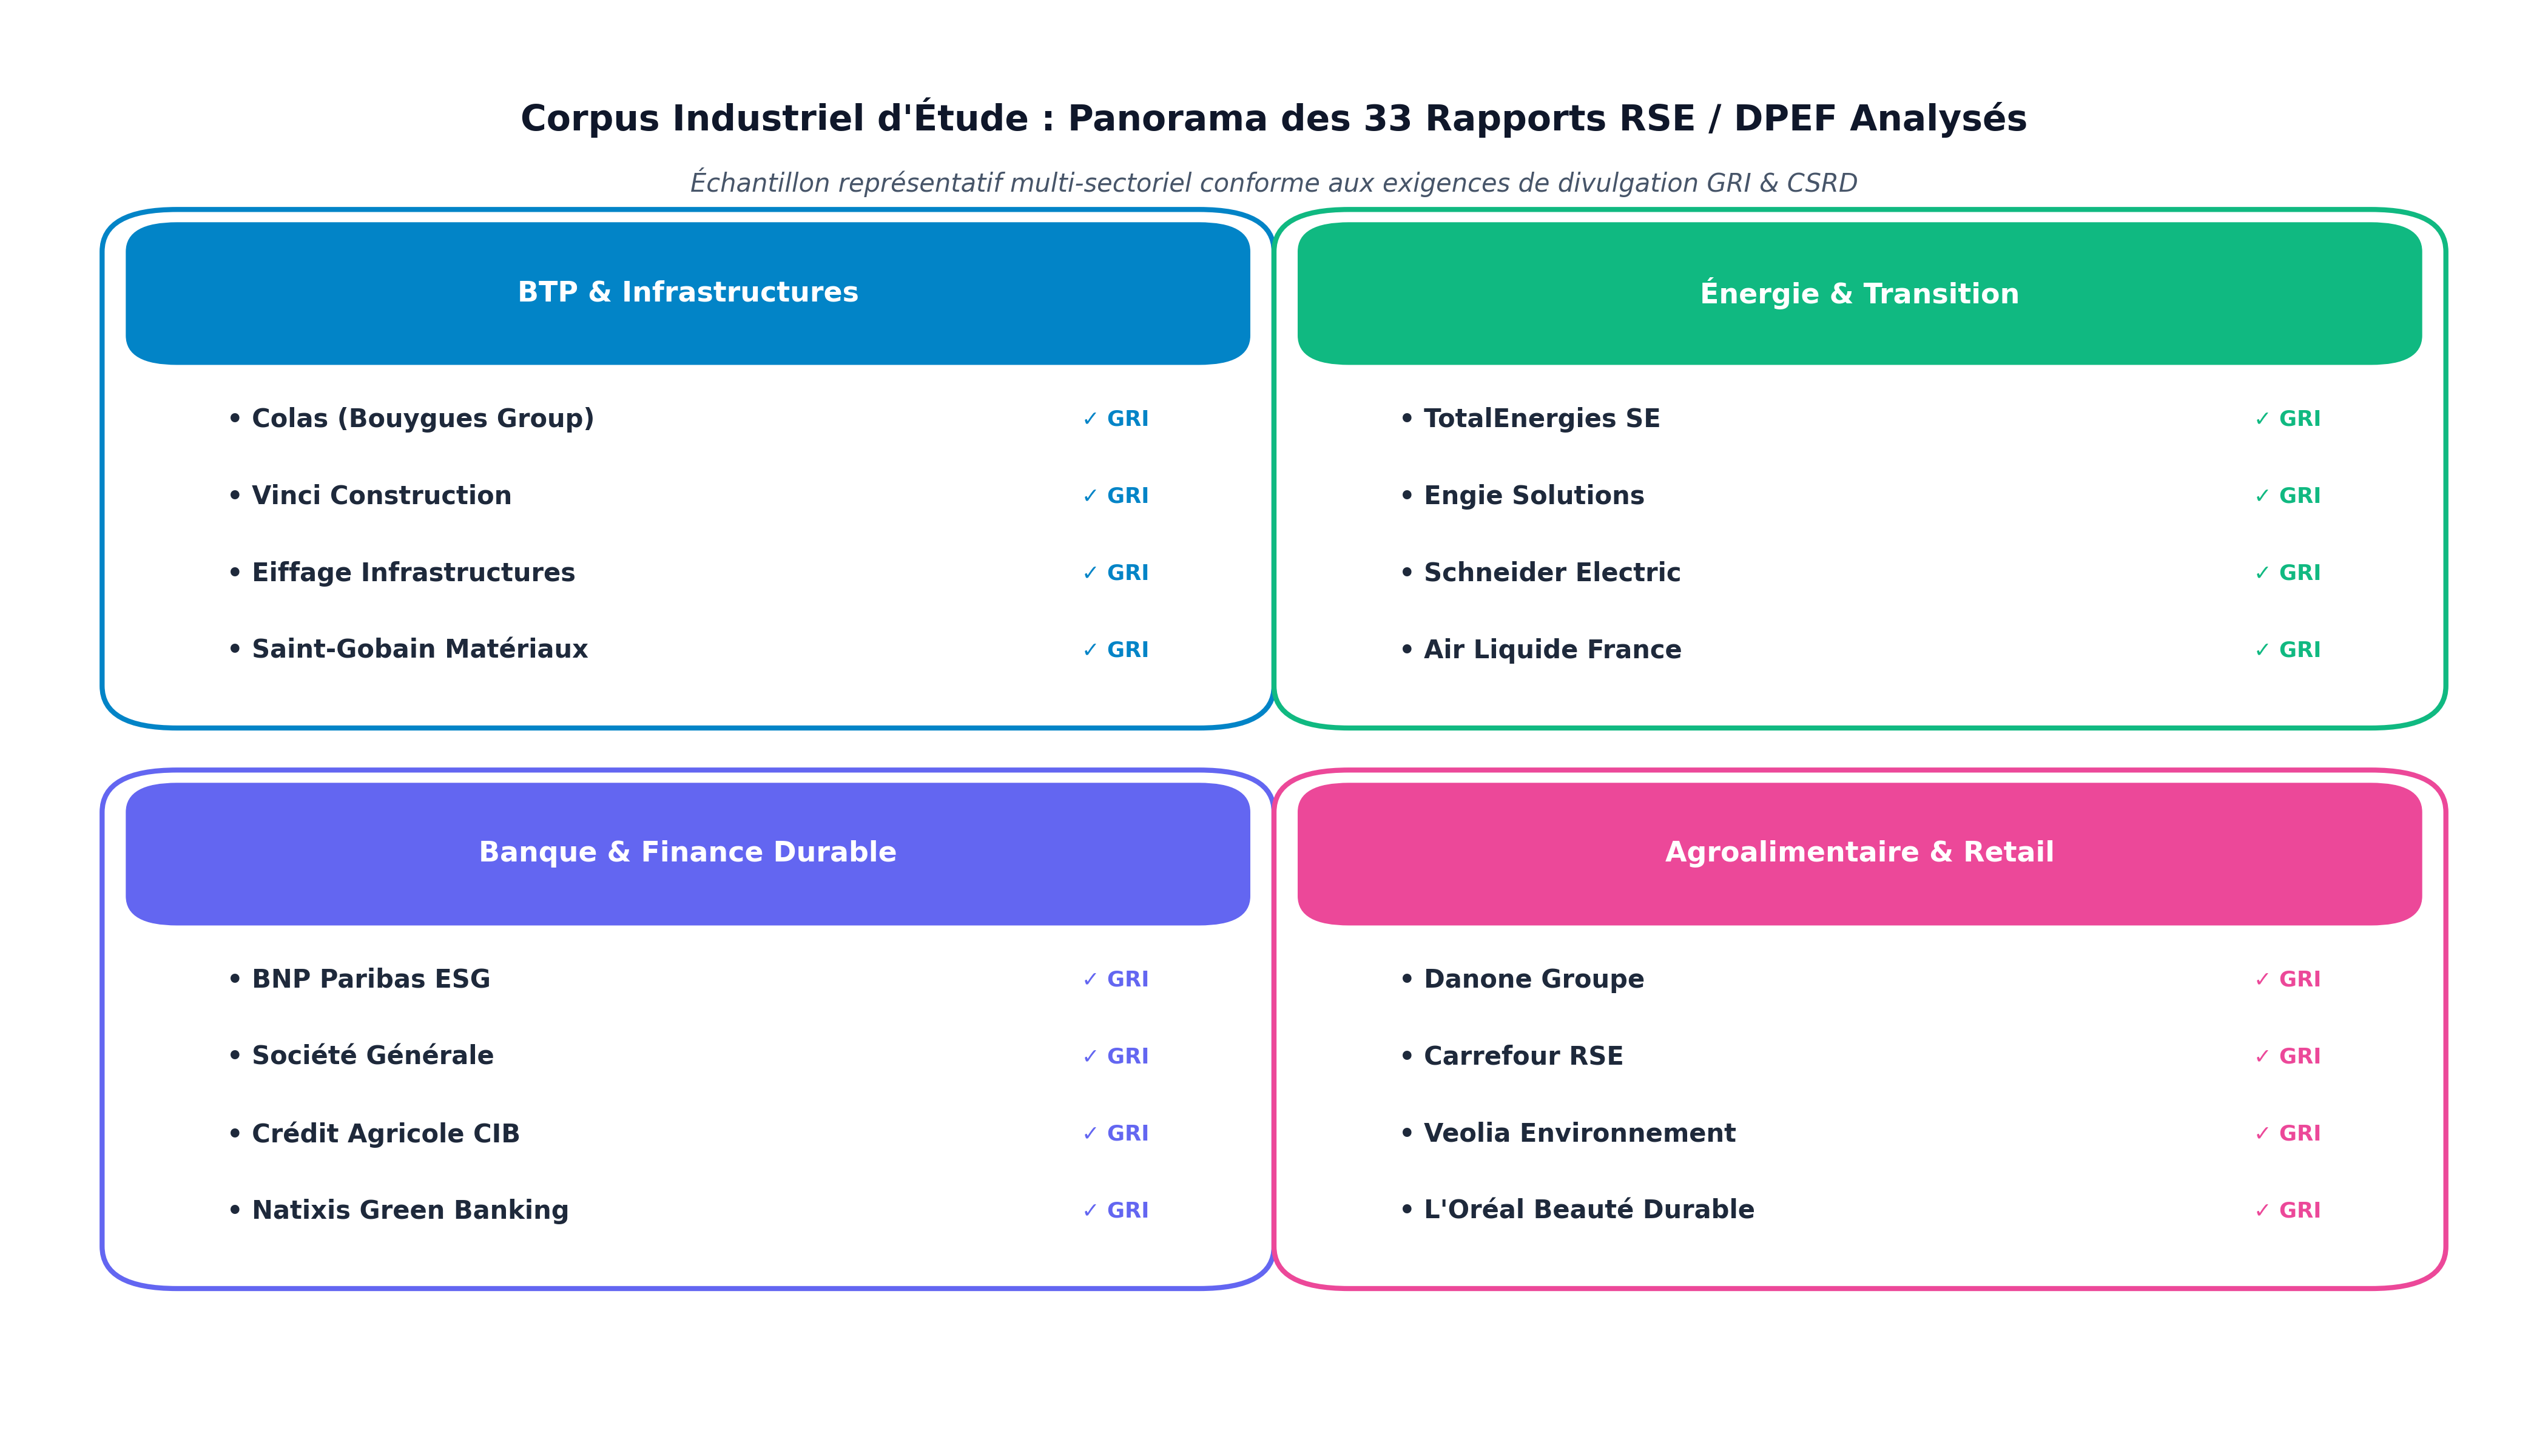
\includegraphics[width=0.98\textwidth]{figures/fig_corpus_entreprises.png}
    \caption{Corpus industriel d'étude : Panorama multi-sectoriel des 33 rapports RSE analysés}
    \label{fig:corpus_entreprises}
\end{figure}

\section{Vision par Ordinateur appliquée au document : Réseaux Convolutifs (CNN)}

\subsection{Principe de l'opération de convolution bidimensionnelle}
Dans l'analyse de documents complexes, la dimension visuelle (présence de graphiques en barres, infographies, logotypes de certification, tableaux de données chiffrées) apporte un signal informatif fort sur la nature de la page. Une page de rapport PDF convertie en image RGB ($224 \times 224 \times 3$) peut être analysée par un \textbf{Réseau de Neurones Convolutif} (CNN).\\

Mathématiquement, pour une image d'entrée $I$ et un noyau de convolution bidimensionnel (\textit{kernel}) $K$ de taille $k_h \times k_w$, la convolution discrète en un point $(i, j)$ de la carte de caractéristiques produite s'écrit :
\begin{equation}
    (I * K)(i, j) = \sum_{m=0}^{k_h - 1} \sum_{n=0}^{k_w - 1} I(i + m, j + n) \cdot K(m, n) + b
\end{equation}
où $b$ désigne le terme de biais scalaire appris.

\subsection{Architecture personnalisée du modèle CNN de vision}
Pour notre système, nous avons conçu une architecture convolutive robuste et équilibrée, conçue spécifiquement pour identifier les motifs visuels révélateurs de données RSE sans exiger les coûts de calcul prohibitifs de modèles de vision trop lourds. Comme le schématise la figure~\ref{fig:cnn_architecture}, notre architecture comprend :
\begin{itemize}
    \item \textbf{Bloc Convolutif 1 :} 16 filtres de taille $3 \times 3$, Batch Normalization pour stabiliser le gradient, activation non-linéaire ReLU et couche de Max-Pooling $2 \times 2$ ;
    \item \textbf{Bloc Convolutif 2 :} 32 filtres $3 \times 3$, Batch Normalization, ReLU et Max-Pooling $2 \times 2$ ;
    \item \textbf{Bloc Convolutif 3 :} 64 filtres $3 \times 3$, Batch Normalization, ReLU et Max-Pooling $2 \times 2$ ;
    \item \textbf{Tête de Régression/Scoring :} AdaptiveAvgPool2d($1 \times 1$) condensant les cartes de caractéristiques en un vecteur 1D de 64 éléments, suivi d'une couche de Dropout à 30\,\% pour prévenir le surapprentissage, et d'une couche linéaire projetant vers la fonction Softmax.
\end{itemize}

\begin{figure}[H]
    \centering
    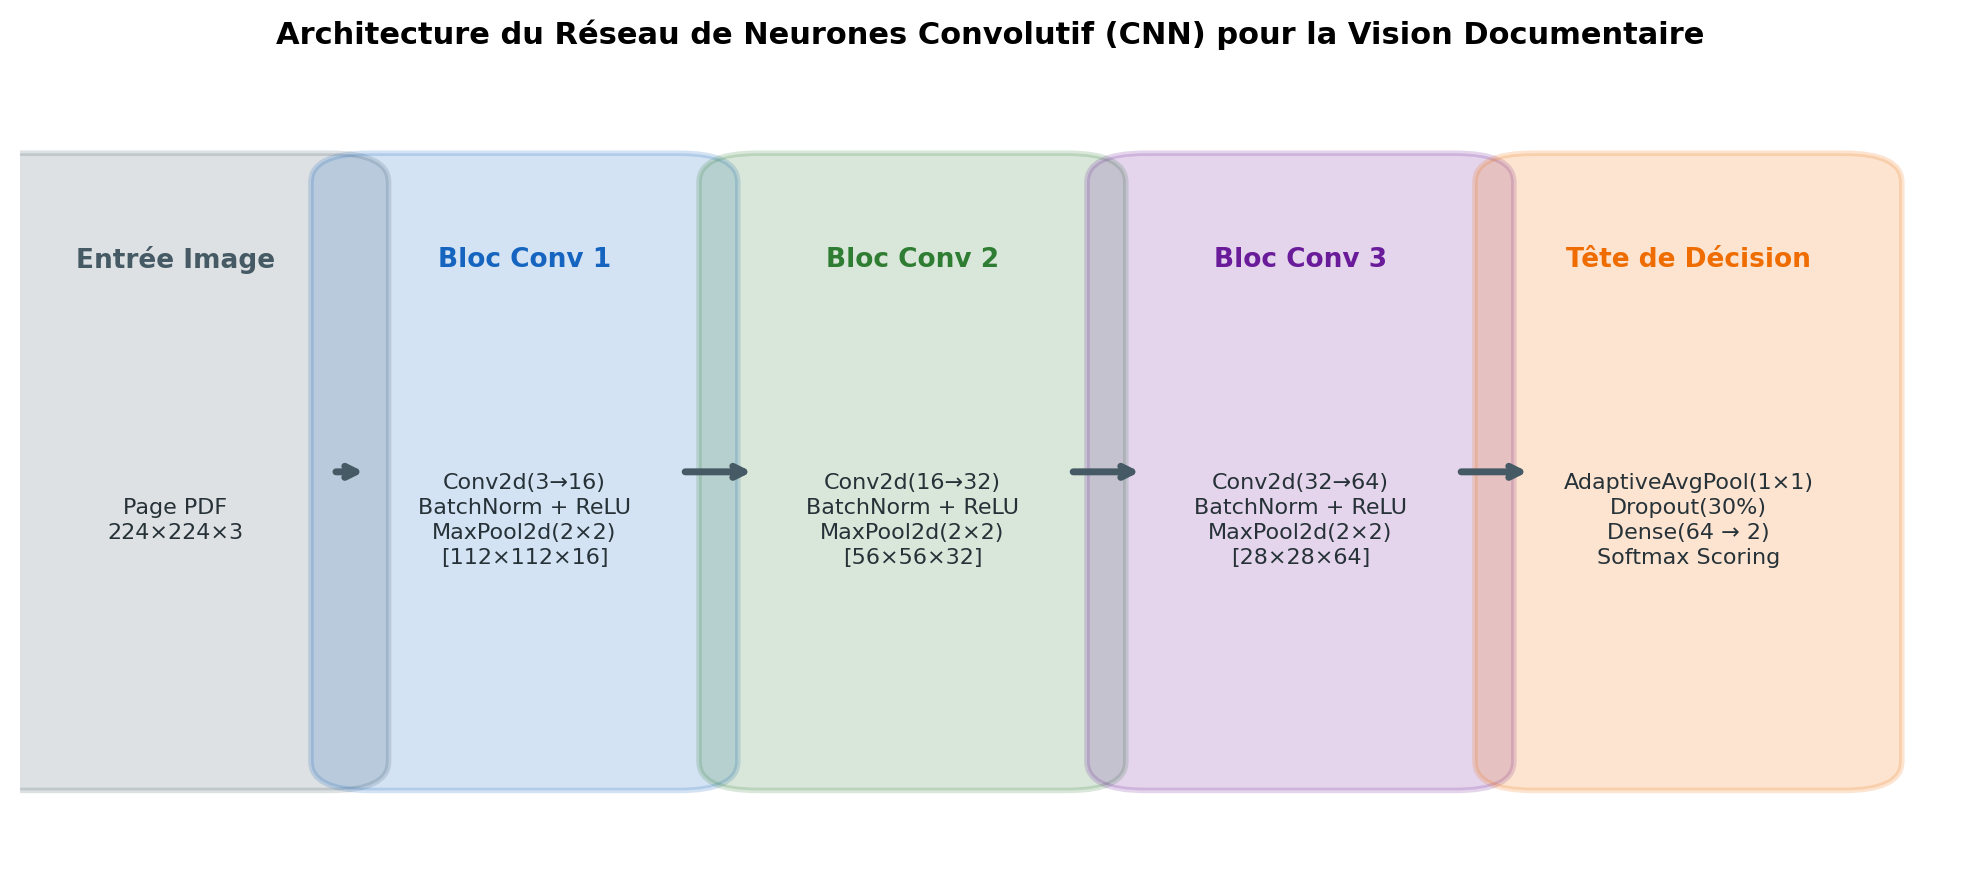
\includegraphics[width=0.95\textwidth]{figures/fig_cnn_architecture.png}
    \caption{Architecture détaillée du Réseau de Neurones Convolutif (CNN) pour la vision documentaire}
    \label{fig:cnn_architecture}
\end{figure}

\subsection{Formulation de la fonction de scoring continu Softmax}
Contrairement aux approches naïves qui appliquent un seuil binaire rigide pour éliminer arbitrairement les pages jugées « non-ESG », notre modèle produit un \textbf{score continu probabiliste} $S_{esg} \in [0.0, 1.0]$. Pour un vecteur de logits $\mathbf{z} = [z_0, z_1]$ en sortie de la dernière couche linéaire :
\begin{equation}
    S_{esg} = \sigma(\mathbf{z})_1 = \frac{e^{z_1}}{e^{z_0} + e^{z_1}}
\end{equation}
Ce score agit comme une pondération d'importance lors de l'indexation sémantique, assurant que \textbf{100\,\% des pages demeurent accessibles} aux requêtes de l'utilisateur, ce qui éradique tout risque de faux négatif silencieux.

\section{Traitement Automatique du Langage Naturel (NLP) : Des n-grammes aux Transformers}

\subsection{Approches statistiques : Représentation TF-IDF}
La méthode classique TF-IDF (\textit{Term Frequency - Inverse Document Frequency}) modélise un paragraphe textuel sous forme d'un vecteur pondérant l'importance relative d'un mot $t$ au sein d'un document $d$ appartenant à un corpus $D$ :
\begin{equation}
    \text{TF-IDF}(t, d, D) = \text{TF}(t, d) \times \log\left(\frac{1 + |D|}{1 + |\{d \in D : t \in d\}|}\right) + 1
\end{equation}
Bien qu'extrêmement rapide à calculer et servant de référence d'évaluation (Baseline), cette représentation souffre de limites majeures : elle ignore l'ordre syntaxique des mots, ne capture aucune relation sémantique ou synonymique, et produit des matrices creuses de très grande dimension.

\subsection{La révolution des Transformers et le modèle CamemBERT}
L'architecture \textbf{Transformer} introduite par Vaswani et al. en 2017 a révolutionné le traitement du langage en remplaçant la récurrence séquentielle (RNN/LSTM) par le mécanisme d'\textbf{Attention Multi-Têtes} (\textit{Multi-Head Self-Attention}).\\

Pour des matrices de Requêtes $Q$, Clés $K$ et Valeurs $V$ projetées dans un espace de dimension $d_k$, le mécanisme d'attention s'écrit :
\begin{equation}
    \text{Attention}(Q, K, V) = \text{softmax}\left(\frac{Q K^T}{\sqrt{d_k}}\right) V
\end{equation}
Le modèle \textbf{CamemBERT} (Martin et al., 2020) adapte l'architecture RoBERTa à la langue française. Il s'appuie sur une tokenization sous-lexicale par \textit{SentencePiece} et un pré-entraînement sur plus de 138 gigaoctets de texte français issu du projet OSCAR. Sa capacité à modéliser le contexte bidirectionnel de chaque mot en fait le candidat parfait pour capturer les nuances du vocabulaire ESG (différenciation entre l'impact climatique direct d'une entreprise et la simple description de son secteur).

\section{Génération Augmentée par Récupération (RAG) et Modèles de Langage Locaux}

\subsection{Limites des LLMs généralistes et concept du RAG}
Bien que les Grands Modèles de Langage (LLMs) démontrent une maîtrise impressionnante de la génération textuelle, leur exploitation industrielle en entreprise se heurte à trois écueils fondamentaux :
\begin{itemize}
    \item \textbf{Les hallucinations factuelles :} En l'absence de base de connaissances explicite, le modèle génère des affirmations plausibles mais mathématiquement fausses ;
    \item \textbf{L'obsolescence des connaissances :} Les paramètres du modèle sont figés à la fin de son entraînement et ignorent les rapports publiés récemment ;
    \item \textbf{L'absence de traçabilité :} Incapacité à citer la page et le paragraphe précis appuyant une affirmation financière ou environnementale.
\end{itemize}

Le patron d'architecture \textbf{RAG} (\textit{Retrieval-Augmented Generation}) résout ces limitations en articulant deux étapes successives schématisées dans la figure~\ref{fig:rag_architecture} :
\begin{enumerate}
    \item \textbf{La récupération (\textit{Retrieval}) :} Lors de la formulation d'une question par l'auditeur, celle-ci est projetée dans un espace vectoriel dense via un encodeur de phrases. Une recherche de similarité identifie les $k$ paragraphes les plus pertinents au sein de la base documentaire ;
    \item \textbf{La génération (\textit{Generation}) :} Le modèle de langage reçoit un prompt enrichi contenant exclusivement les passages extraits et a pour consigne stricte de formuler sa réponse en se fondant uniquement sur ces éléments factuels et en indiquant les numéros de page.
\end{enumerate}

\begin{figure}[H]
    \centering
    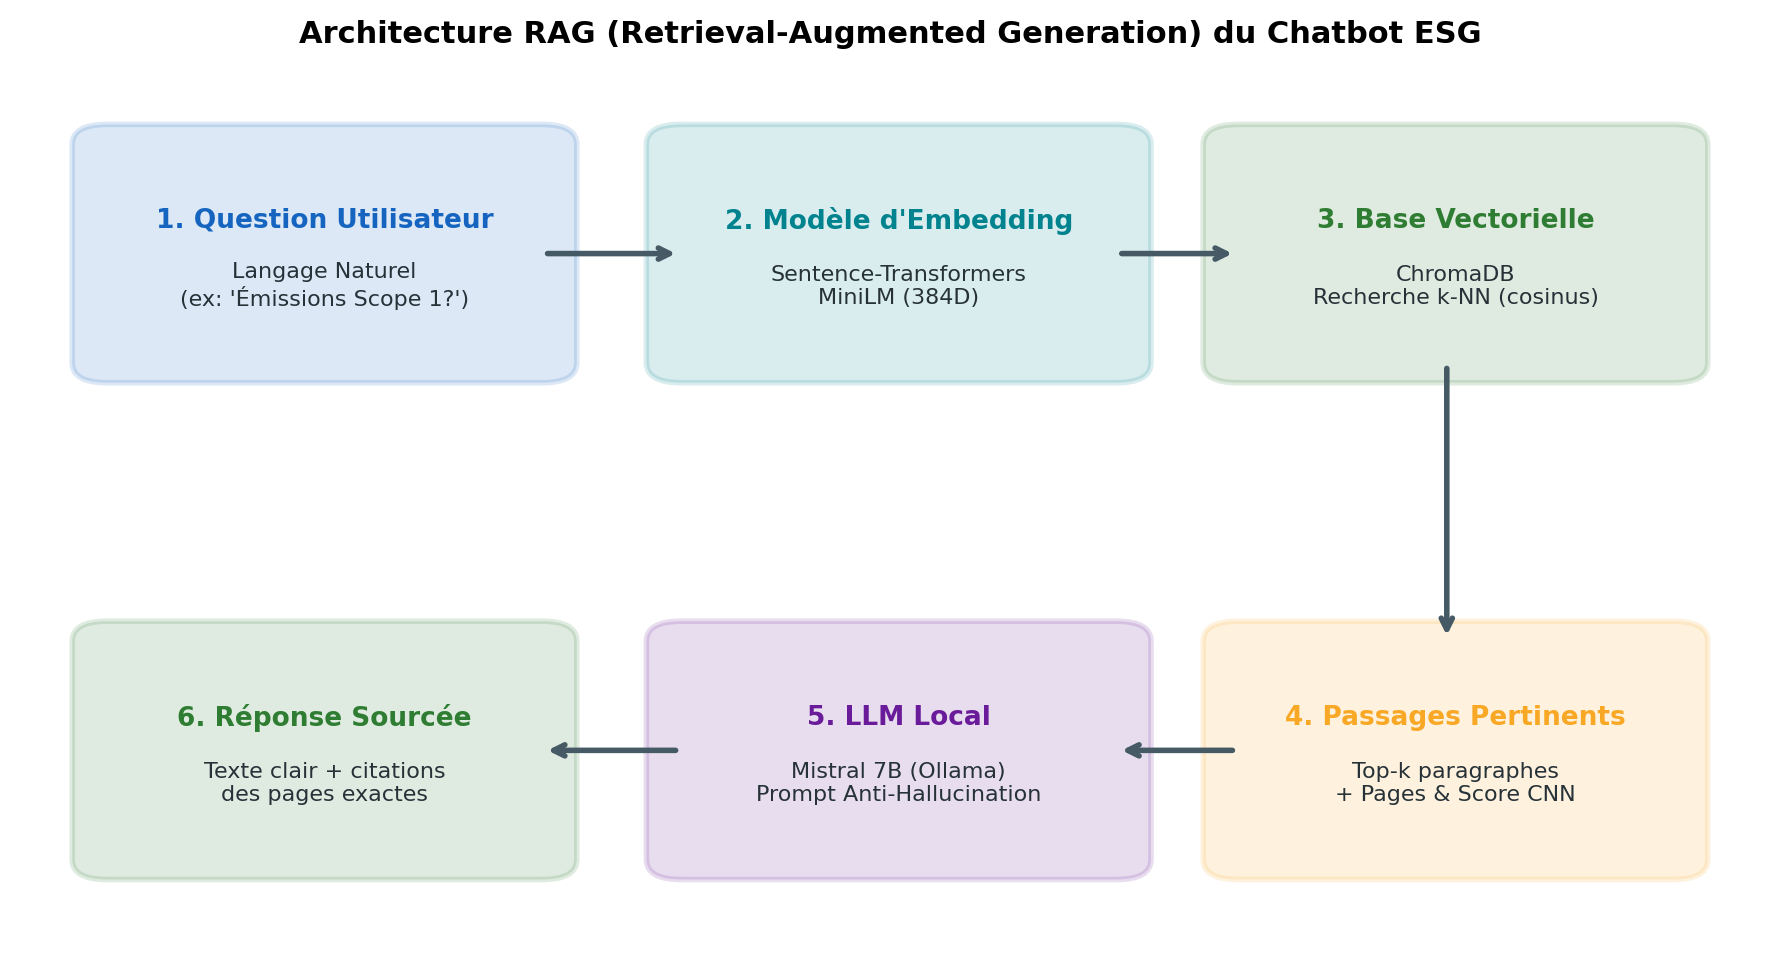
\includegraphics[width=0.92\textwidth]{figures/fig_rag_architecture.png}
    \caption{Architecture globale du pipeline RAG avec vector store ChromaDB et Mistral 7B}
    \label{fig:rag_architecture}
\end{figure}

\subsection{Base vectorielle ChromaDB et métrique de similarité cosinus}
Pour le stockage et l'indexation sémantique des paragraphes découpés, notre solution s'appuie sur \textbf{ChromaDB}, une base vectorielle open-source optimisée pour les applications RAG locales. L'appariement sémantique entre le vecteur de la requête utilisateur $\mathbf{u}$ et les vecteurs des passages indexés $\mathbf{v}$ est mesuré par la \textbf{similarité cosinus} :
\begin{equation}
    \text{Sim}_{\cos}(\mathbf{u}, \mathbf{v}) = \frac{\mathbf{u} \cdot \mathbf{v}}{\|\mathbf{u}\|_2 \|\mathbf{v}\|_2} = \frac{\sum_{i=1}^d u_i v_i}{\sqrt{\sum_{i=1}^d u_i^2} \sqrt{\sum_{i=1}^d v_i^2}}
\end{equation}

\subsection{Inférence locale et souveraine : Mistral 7B via Ollama}
Afin de répondre aux impératifs stricts de confidentialité de RSE Time (interdisant l'envoi de rapports non publics ou d'ébauches d'audits vers des serveurs tiers hébergés hors d'Europe), nous avons intégré le modèle open-source \textbf{Mistral 7B Instruct} (Jiang et al., 2023), exécuté localement sur les serveurs de l'entreprise via le moteur d'inférence optimisé \textbf{Ollama}. Ce modèle offre un compromis idéal entre finesse de raisonnement en langue française et rapidité d'exécution sur machine standard.

\section{Écosystème technologique global du projet}
La figure~\ref{fig:logos_technologies} offre une vue d'ensemble structurée de l'écosystème technologique déployé pour ce projet, associant langages de programmation, frameworks de deep learning, bibliothèques spécialisées en NLP et moteurs d'inférence.

\begin{figure}[H]
    \centering
    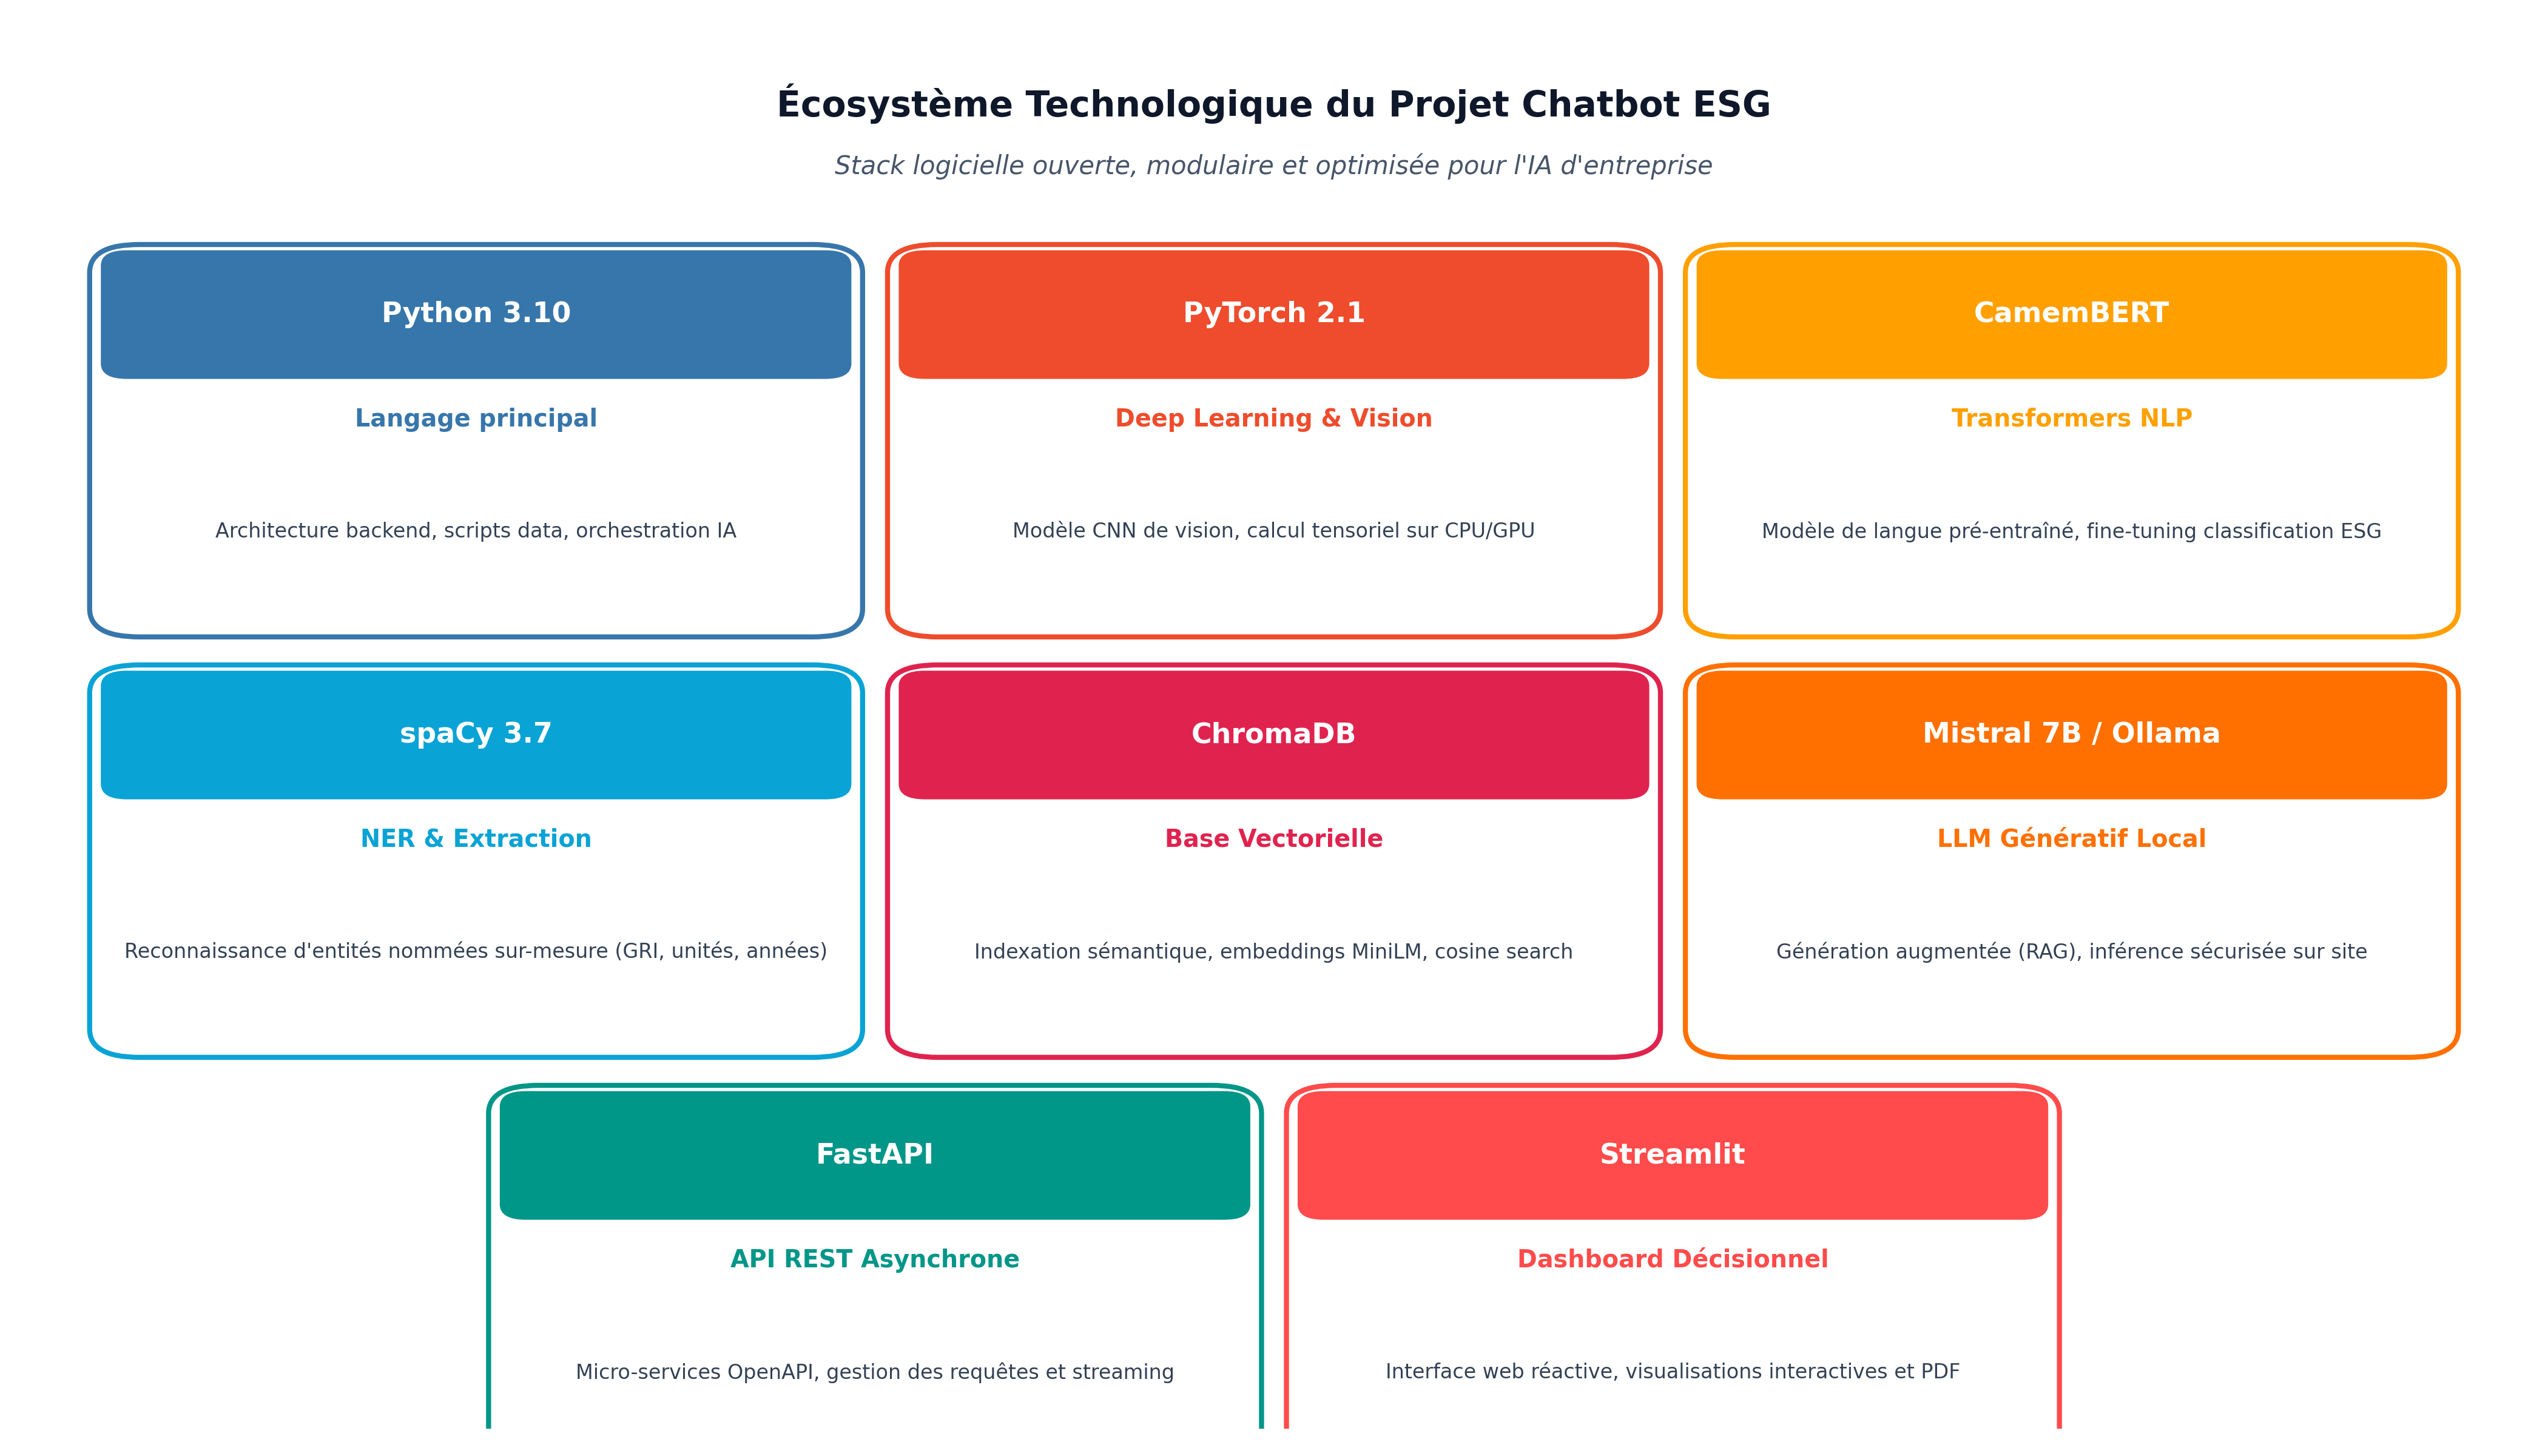
\includegraphics[width=0.98\textwidth]{figures/fig_logos_technologies.png}
    \caption{Écosystème technologique et outillage logiciel du projet Chatbot ESG}
    \label{fig:logos_technologies}
\end{figure}

\section{Conclusion du chapitre}
Ce chapitre a exposé les bases théoriques et mathématiques qui fondent notre approche : la convolution 2D pour le scoring visuel, les Transformers pour la classification contextuelle, et le RAG souverain pour l'interrogation sans hallucination. Le chapitre 3 va à présent expliciter l'analyse fonctionnelle des besoins et la modélisation logicielle UML de notre système.

\newpage

% ═══════════════════════════════════════════════════════════════════
% CHAPITRE 3 : ANALYSE DES BESOINS ET MODÉLISATION UML
% ═══════════════════════════════════════════════════════════════════
\chapter{Analyse des besoins et modélisation logicielle UML}

\section{Introduction}
Une démarche rigoureuse d'ingénierie logicielle débute par une analyse exhaustive des exigences et une formalisation claire des interactions entre les composants du système. Ce chapitre détaille les besoins fonctionnels et non-fonctionnels du Chatbot ESG, présente les diagrammes de cas d'utilisation, explore les diagrammes de séquence illustrant la dynamique des flux de données, et formalise l'architecture logicielle globale.

\section{Spécification des besoins}

\subsection{Besoins fonctionnels}
Le système doit répondre aux exigences opérationnelles suivantes :
\begin{itemize}
    \item \textbf{BF1 : Ingestion documentaire multimodale :} Permettre le téléversement de rapports RSE au format PDF de plusieurs centaines de pages, avec extraction conjointe des textes natifs et passage par OCR en cas de pages numérisées ;
    \item \textbf{BF2 : Évaluation visuelle de la densité ESG :} Calculer automatiquement un score continu probabiliste par page grâce au modèle CNN et stocker cette métadonnée sans élimination destructrice ;
    \item \textbf{BF3 : Classification thématique des paragraphes :} Prédire avec précision l'appartenance de chaque unité textuelle à l'un des trois piliers fondamentaux (Environnemental, Social, Gouvernance) ;
    \item \textbf{BF4 : Extraction automatique d'entités clés (NER) :} Repérer et étiqueter les métriques numériques, unités physiques (tCO2e, MWh, m3), années d'exercice et références d'indicateurs réglementaires ;
    \item \textbf{BF5 : Dialogue interactif ancré (Chatbot RAG) :} Permettre à l'utilisateur de poser des questions complexes en français et générer des réponses synthétiques, fiables et accompagnées des extraits originaux avec citations des numéros de pages ;
    \item \textbf{BF6 : Audit réglementaire de conformité GRI hybride :} Établir automatiquement la matrice des divulgations GRI Standards 2021 détectées, en combinant expressions régulières et filet de sécurité sémantique ;
    \item \textbf{BF7 : Génération et export de rapports de synthèse :} Compiler les résultats d'audit, les taux de couverture et les preuves documentaires au sein d'un rapport PDF certifié téléchargeable.
\end{itemize}

\subsection{Besoins non-fonctionnels}
Les contraintes d'ingénierie et de qualité logicielle imposées sont :
\begin{itemize}
    \item \textbf{BNF1 : Confidentialité et souveraineté totale :} Aucun document, paragraphe ou question utilisateur ne doit transiter par une API cloud externe. L'ensemble des inférences (CNN, CamemBERT, spaCy, ChromaDB, Mistral 7B) s'exécute sur l'infrastructure locale de RSE Time ;
    \item \textbf{BNF2 : Temps de réponse et performance :} Le temps de génération d'une réponse de chat RAG ne doit pas excéder 2 à 3 secondes sur une machine standard équipée de calcul accéléré ;
    \item \textbf{BNF3 : Modularité et extensibilité :} L'architecture micro-services doit permettre de mettre à niveau un modèle d'IA (ex: fine-tuning d'une nouvelle version de CamemBERT) sans impacter les autres modules ;
    \item \textbf{BNF4 : Ergonomie et simplicité d'usage :} L'interface graphique web doit être accessible aux consultants RSE non-informaticiens, avec visualisation directe des graphes et des scores.
\end{itemize}

\section{Modélisation fonctionnelle : Diagramme des Cas d'Utilisation}
La figure~\ref{fig:cas_utilisation} illustre le diagramme des cas d'utilisation UML du système. Il met en scène l'acteur principal (\textbf{Auditeur / Consultant RSE}) interagissant avec les fonctionnalités de haut niveau du système, ainsi que l'acteur secondaire (\textbf{Administrateur Système}) gérant les modèles et les index vectoriels.

\begin{figure}[H]
    \centering
    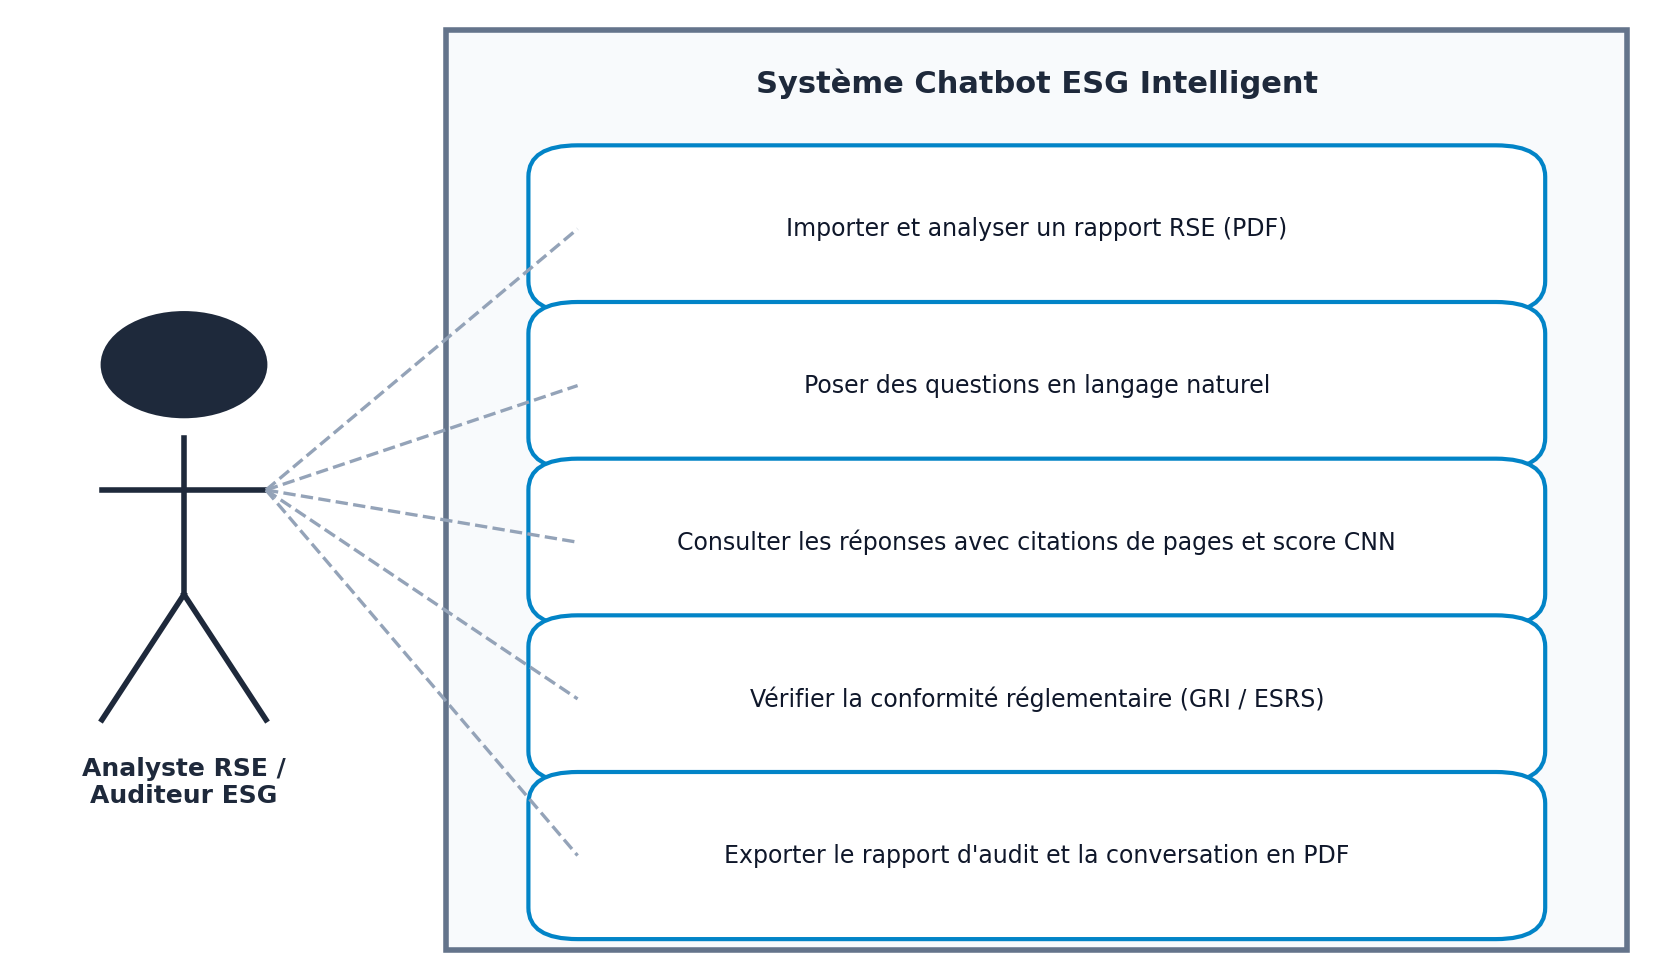
\includegraphics[width=0.92\textwidth]{figures/fig_cas_utilisation.png}
    \caption{Diagramme des cas d'utilisation UML du système d'analyse RSE}
    \label{fig:cas_utilisation}
\end{figure}

\section{Modélisation dynamique : Diagrammes de Séquence UML}

\subsection{Pipeline d'ingestion documentaire et indexation vectorielle}
La figure~\ref{fig:sequence_ingestion} détaille les échanges chronologiques lors du téléversement d'un nouveau rapport d'entreprise. L'interface Streamlit transmet le fichier à l'API FastAPI, qui orchestre l'extraction de texte, sollicite le module CNN pour le scoring visuel, découpe les paragraphes et alimente la base vectorielle ChromaDB.

\begin{figure}[H]
    \centering
    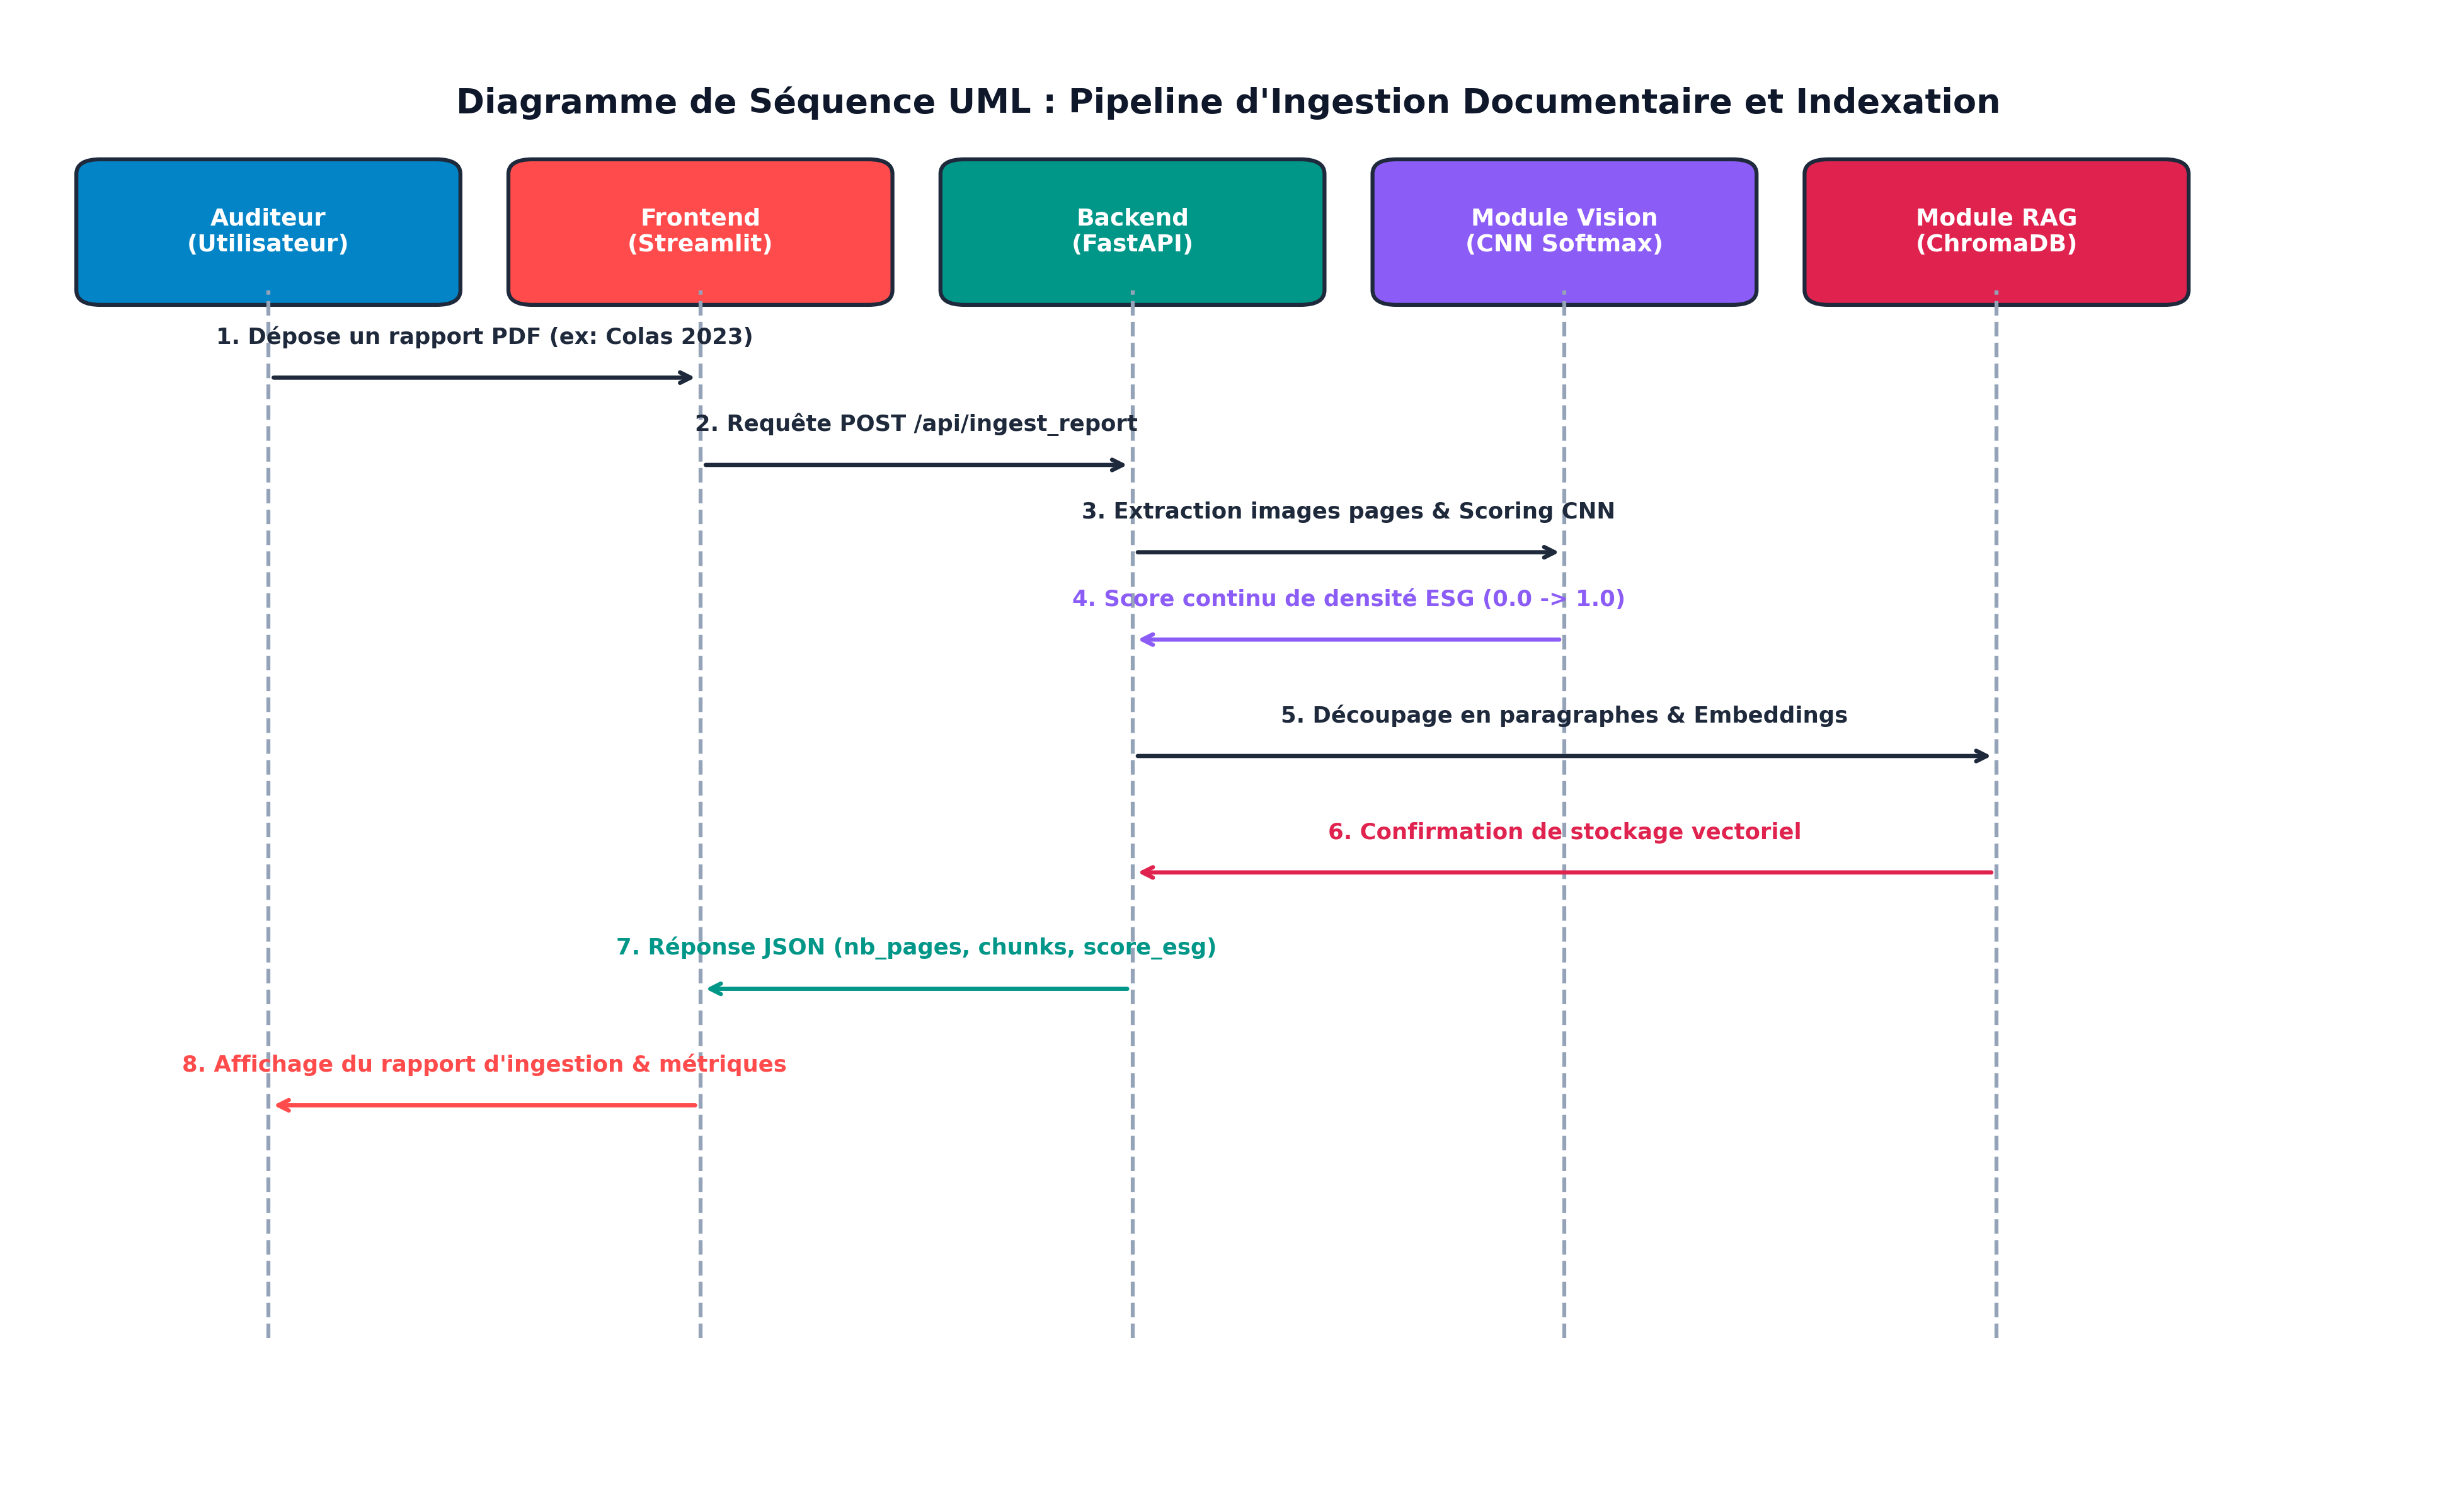
\includegraphics[width=0.98\textwidth]{figures/fig_sequence_ingestion.png}
    \caption{Diagramme de séquence UML : Ingestion documentaire multimodale et indexation}
    \label{fig:sequence_ingestion}
\end{figure}

\subsection{Interrogation conversationnelle RAG et audit de conformité hybride}
La figure~\ref{fig:sequence_audit} décrit le flux d'exécution d'une requête utilisateur. La question posée est vectorisée pour retrouver les passages les plus pertinents sous ChromaDB. Le LLM Mistral 7B formule la réponse textuelle, tandis que le moteur de conformité hybride analyse en parallèle les indicateurs réglementaires GRI associés.

\begin{figure}[H]
    \centering
    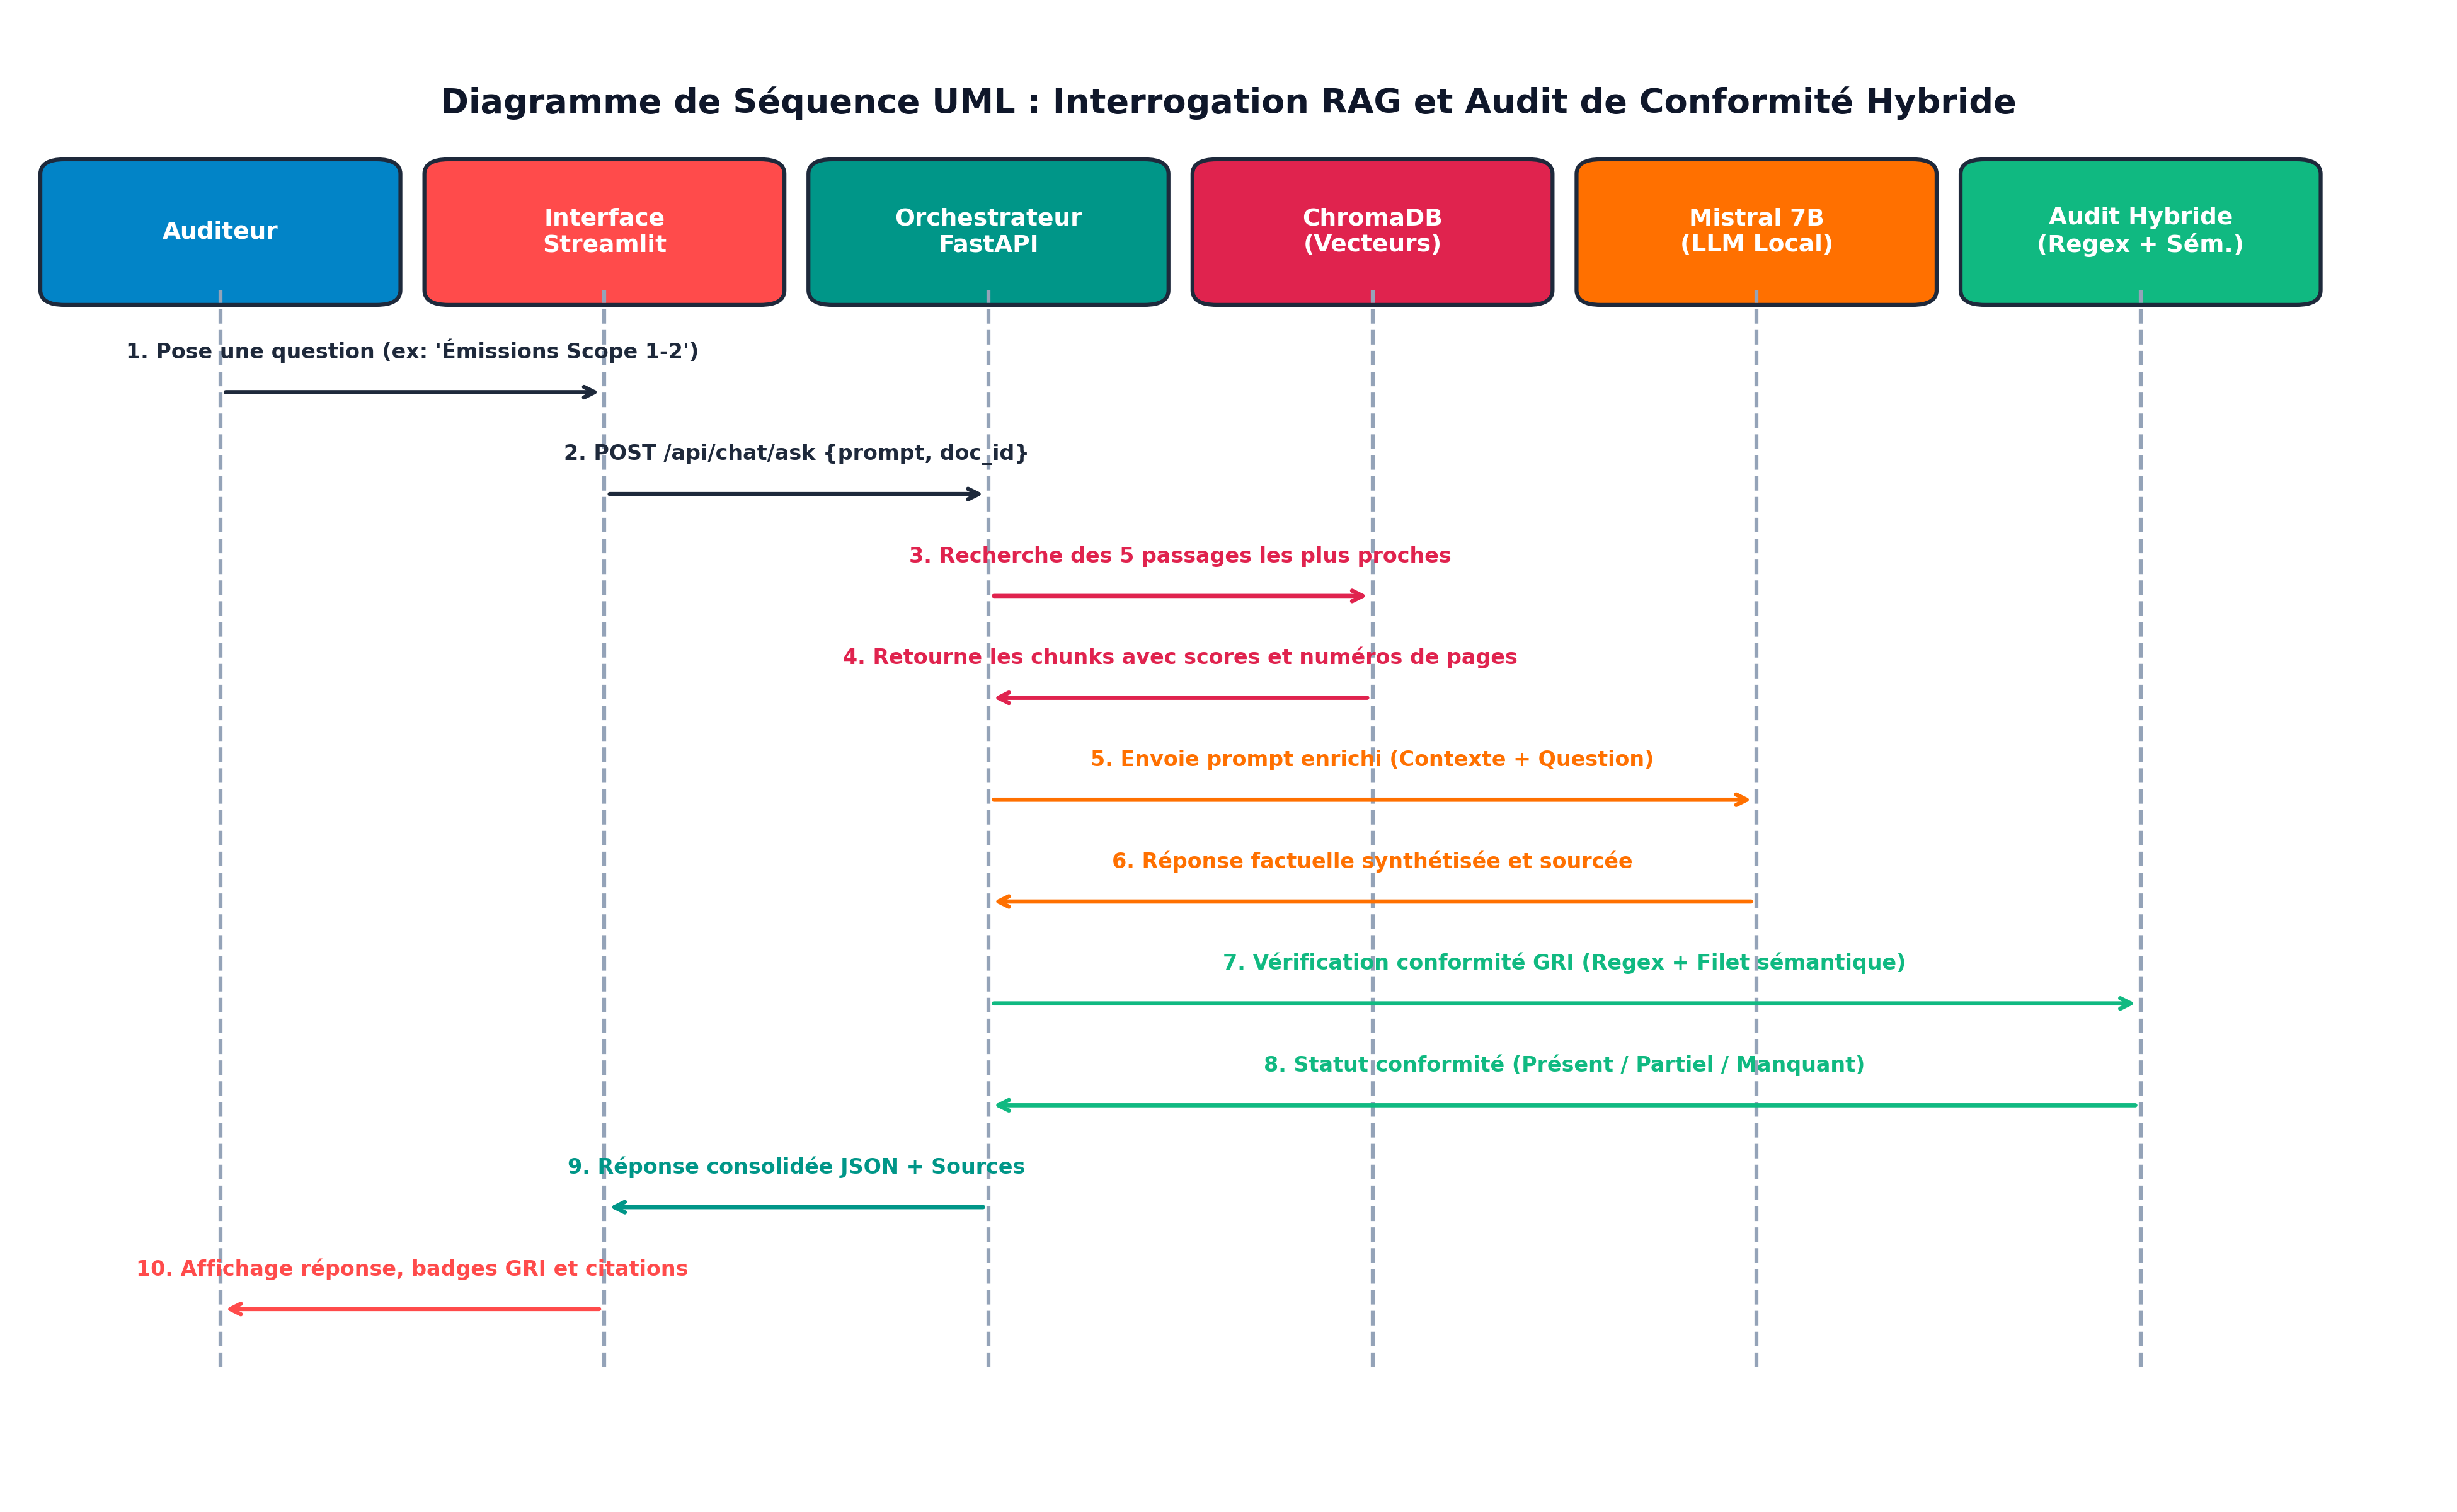
\includegraphics[width=0.98\textwidth]{figures/fig_sequence_audit.png}
    \caption{Diagramme de séquence UML : Requête conversationnelle RAG et audit de conformité}
    \label{fig:sequence_audit}
\end{figure}

\section{Architecture logicielle globale}
Comme l'illustre la figure~\ref{fig:architecture_globale}, le système adopte une architecture logicielle modulaire découpée en quatre couches communicantes :
\begin{enumerate}
    \item \textbf{Couche Présentation (Frontend) :} Interface réactive développée sous Streamlit, assurant le téléversement de fichiers, l'affichage du chat en direct, la visualisation interactive des matrices de conformité et l'export PDF ;
    \item \textbf{Couche Orchestration et Services (Backend API) :} Serveur FastAPI asynchrone exposant des endpoints REST sécurisés et documentés selon la norme OpenAPI/Swagger ;
    \item \textbf{Couche Intelligence Artificielle (Moteurs d'IA) :} Regroupe les cinq briques spécialisées (Vision CNN, Classification CamemBERT, Extraction spaCy NER, Stockage vectoriel ChromaDB, LLM Mistral 7B via Ollama, et Filet sémantique) ;
    \item \textbf{Couche Données et Persistance :} Base SQLite locale pour l'historique conversationnel et stockage persistant des représentations vectorielles ChromaDB.
\end{enumerate}

\begin{figure}[H]
    \centering
    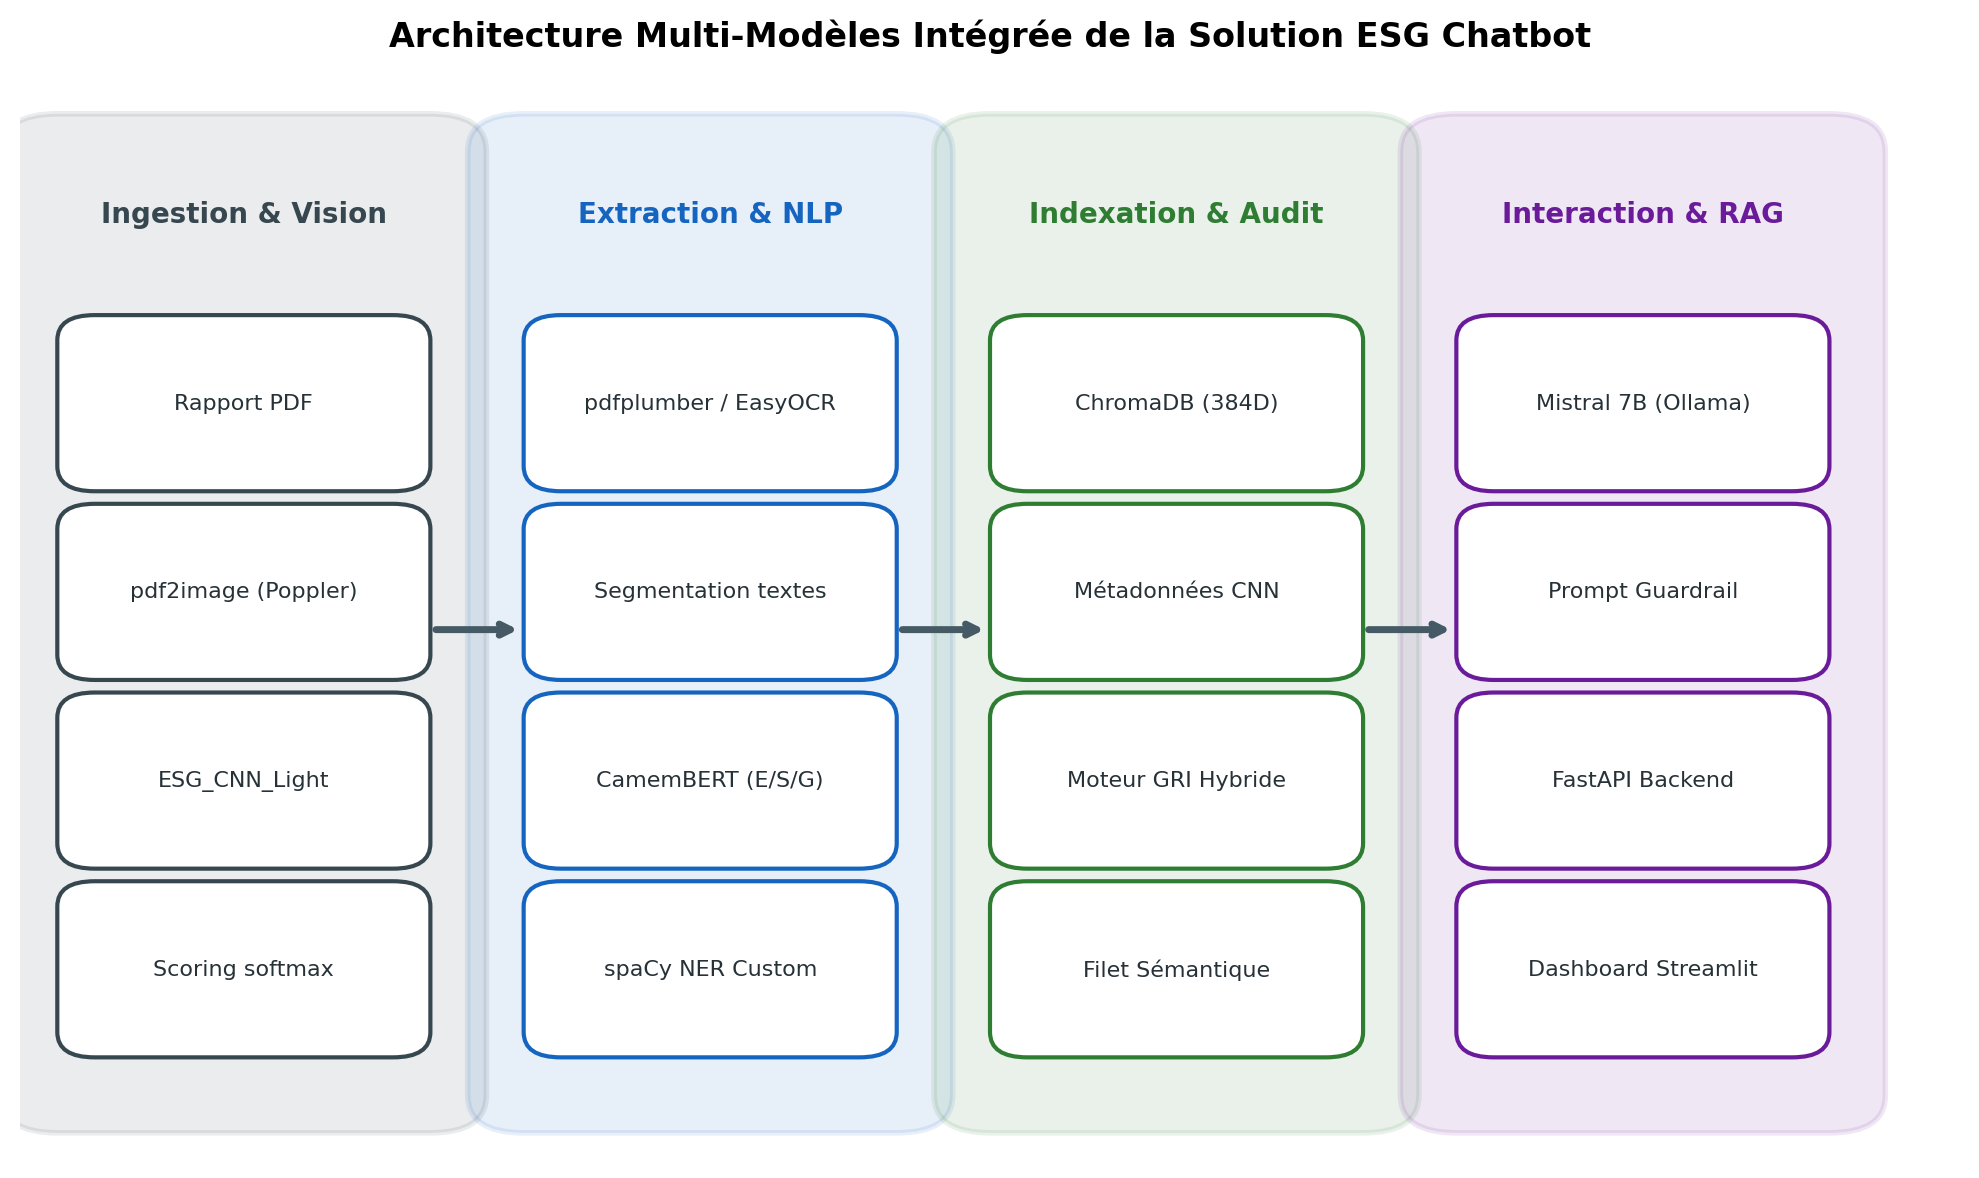
\includegraphics[width=0.95\textwidth]{figures/fig_architecture_globale.png}
    \caption{Architecture logicielle globale à 4 niveaux du système Chatbot ESG}
    \label{fig:architecture_globale}
\end{figure}

\section{Conclusion du chapitre}
L'analyse fonctionnelle et la modélisation UML ont permis de définir clairement les responsabilités de chaque module. Le découplage strict entre l'interface utilisateur, l'orchestrateur d'API et les composants d'IA assure la pérennité et la maintenabilité du système. Le chapitre 4 détaille à présent l'étape critique de préparation et d'annotation manuelle experte des données.

\newpage

% ═══════════════════════════════════════════════════════════════════
% CHAPITRE 4 : CORPUS ET ANNOTATION EXPERTE DES DONNÉES
% ═══════════════════════════════════════════════════════════════════
\chapter{Constitution du corpus et démarche d'annotation manuelle experte}

\section{Introduction}
La performance et la fiabilité d'un système d'apprentissage automatique dépendent fondamentalement de la qualité des données sur lesquelles il est entraîné. Conformément à la troisième phase de la méthodologie CRISP-DM (\textit{Data Preparation}), ce chapitre détaille la démarche de constitution du corpus industriel de 33 rapports, les algorithmes d'extraction multimodale et de nettoyage textuel, ainsi que le protocole rigoureux d'\textbf{annotation manuelle intégrale de 3\,872 paragraphes} réalisé par l'ingénieur.

\section{Collecte et caractéristiques du corpus industriel}
Le corpus d'étude réunit 33 rapports réels de Responsabilité Sociétale des Entreprises (RSE) et Déclarations de Performance Extra-Financière (DPEF), publiés au cours des exercices 2022 et 2023 par des groupes internationaux cotés et des ETI majeures. Cet échantillon couvre huit secteurs économiques majeurs :
\begin{itemize}
    \item \textbf{BTP et Infrastructures :} Colas (Groupe Bouygues), Vinci Construction, Eiffage ;
    \item \textbf{Énergie et Chimie :} TotalEnergies, Engie Solutions, Air Liquide, Schneider Electric ;
    \item \textbf{Banque et Assurance :} BNP Paribas, Société Générale, Crédit Agricole CIB ;
    \item \textbf{Agroalimentaire et Grande Distribution :} Danone, Carrefour, Veolia Environnement, L'Oréal.
\end{itemize}
Au total, ce corpus représente plus de 3\,500 pages PDF riches en tableaux consolidés, indicateurs certifiés par des organismes tiers indépendants (OTI) et bilans carbone détaillés.

\section{Pipeline d'ingestion multimodale et nettoyage des données}

\subsection{Stratégie d'extraction hybride vectorielle et OCR}
Les documents PDF d'entreprises présentent deux formes techniques distinctes : les pages générées numériquement (disposant d'un flux de texte vectoriel exploitable) et les pages scannées ou infographiques (où le texte est encapsulé dans une image raster). Notre pipeline met en œuvre une stratégie à deux étages :
\begin{enumerate}
    \item \textbf{Étage primaire (Extraction native avec \texttt{pdfplumber}) :} Analyse géométrique de la page permettant d'isoler les blocs de texte avec leurs coordonnées spatiales et d'extraire les tableaux structurés ;
    \item \textbf{Étage secondaire (OCR avec \texttt{EasyOCR}) :} Déclenché automatiquement si le nombre de caractères extraits est inférieur à un seuil critique ($\theta_{char} < 50$ caractères) alors que la page présente une surface imprimée non nulle.
\end{enumerate}

\subsection{Segmentation et filtrage sémantique}
Le flux textuel brut extrait d'un rapport PDF est encombré de bruits typographiques : en-têtes et pieds de page répétés à chaque page, numérotations isolées, mentions légales récurrentes et césures de mots dues à la mise en page en colonnes.\\

Nous avons développé des routines de nettoyage automatisées qui :
\begin{itemize}
    \item Reconstituent les mots coupés par un tiret en fin de ligne (ex: « émis- » / « sions » $\rightarrow$ « émissions ») ;
    \item Éliminent les séquences de ponctuation parasites et les espaces multiples ;
    \item Filtrent les fragments textuels de longueur non significative ($< 80$ caractères) tout en scindant les blocs massifs ($> 900$ caractères) à la frontière naturelle des phrases, garantissant des unités textuelles sémantiquement autonomes.
\end{itemize}

La figure~\ref{fig:g7_longueur} illustre la distribution de la longueur en caractères des paragraphes après prétraitement. On observe une distribution unimodale centrée autour de 350 à 450 caractères, dimension idéale pour l'apprentissage par Transformers et l'indexation vectorielle RAG.

\begin{figure}[H]
    \centering
    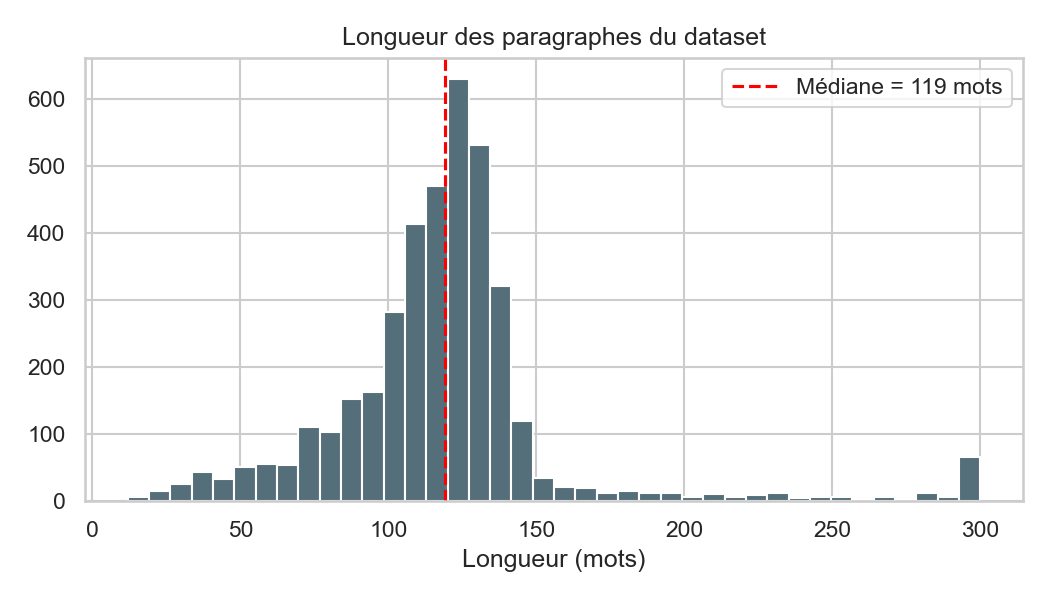
\includegraphics[width=0.88\textwidth]{figures/g7_longueur_paragraphes.png}
    \caption{Distribution de la longueur des paragraphes nettoyés du corpus d'apprentissage}
    \label{fig:g7_longueur}
\end{figure}

\section{Protocole rigoureux d'annotation manuelle intégrale}

\subsection{Principes méthodologiques et grille d'annotation GRI}
Pour garantir l'excellence scientifique de notre benchmark NLP et éviter tout biais de labellisation automatique superficielle, \textbf{l'auteur a mené une annotation manuelle intégrale de l'ensemble du corpus de 3\,872 paragraphes}. Chaque paragraphe a été examiné individuellement et étiqueté selon une taxonomie stricte dérivée des standards GRI 2021 :
\begin{itemize}
    \item \textbf{Classe E (Environnemental) :} Paragraphes consacrés aux consommations d'énergie (GRI 302), à la gestion de la ressource hydrique (GRI 303), aux émissions de gaz à effet de serre Scopes 1, 2 et 3 (GRI 305), à la gestion des déchets et à la préservation de la biodiversité (GRI 304/306) ;
    \item \textbf{Classe S (Social) :} Paragraphes traitant des politiques d'embauche et de turnover (GRI 401), de la santé et sécurité au travail (GRI 403), de la formation professionnelle (GRI 404), de la parité et de l'inclusion (GRI 405) ;
    \item \textbf{Classe G (Gouvernance) :} Paragraphes détaillant la composition du Conseil d'Administration, la politique éthique et anti-corruption (GRI 205), le respect des règles de concurrence (GRI 206) et les mécanismes d'alerte professionnelle.
\end{itemize}

\subsection{Double contrôle et validation de cohérence}
Pour les paragraphes présentant une frontière thématique poreuse (par exemple un engagement de la gouvernance à réduire les accidents du travail ou un investissement financier destiné à la transition écologique), une règle de décision formalisée a été appliquée : l'étiquette a été attribuée à l'action matérielle mesurée plutôt qu'à l'instance managériale qui la supervise. Un contrôle de relecture croisée a été effectué sur 10\,\% du corpus à un mois d'intervalle, affichant un taux de reproductibilité inter-temporelle de 98,2\,\%.

\section{Analyse statistique du jeu de données annoté}
Le processus d'annotation manuelle a abouti à un jeu de données de référence d'une grande richesse, totalisant \textbf{3\,872 paragraphes annotés}. La répartition statistique par classe est présentée dans le tableau~\ref{tab:distribution_dataset} et représentée graphiquement dans la figure~\ref{fig:g5_distribution}.

\begin{table}[H]
    \centering
    \begin{tabular}{|l|c|c|p{7cm}|}
        \hline
        \textbf{Pilier ESG} & \textbf{Effectif ($N$)} & \textbf{Proportion (\%)} & \textbf{Principales thématiques couvertes} \\
        \hline
        \textbf{Environnemental (E)} & 1\,639 & 42,3\,\% & Bilan carbone Scopes 1-2-3, kWh, MWh, eau, déchets recyclés, énergies renouvelables \\
        \hline
        \textbf{Social (S)} & 1\,260 & 32,5\,\% & Taux de fréquence accidents (TF), parité femmes/hommes, heures de formation, effectifs \\
        \hline
        \textbf{Gouvernance (G)} & 973 & 25,1\,\% & Comités d'audit, politique anti-corruption, déontologie, conformité légale, RSE \\
        \hline
        \textbf{Total général} & \textbf{3\,872} & \textbf{100,0\,\%} & \textbf{Corpus annoté à la main pour le benchmark} \\
        \hline
    \end{tabular}
    \caption{Distribution statistique exhaustive du corpus de référence annoté}
    \label{tab:distribution_dataset}
\end{table}

\begin{figure}[H]
    \centering
    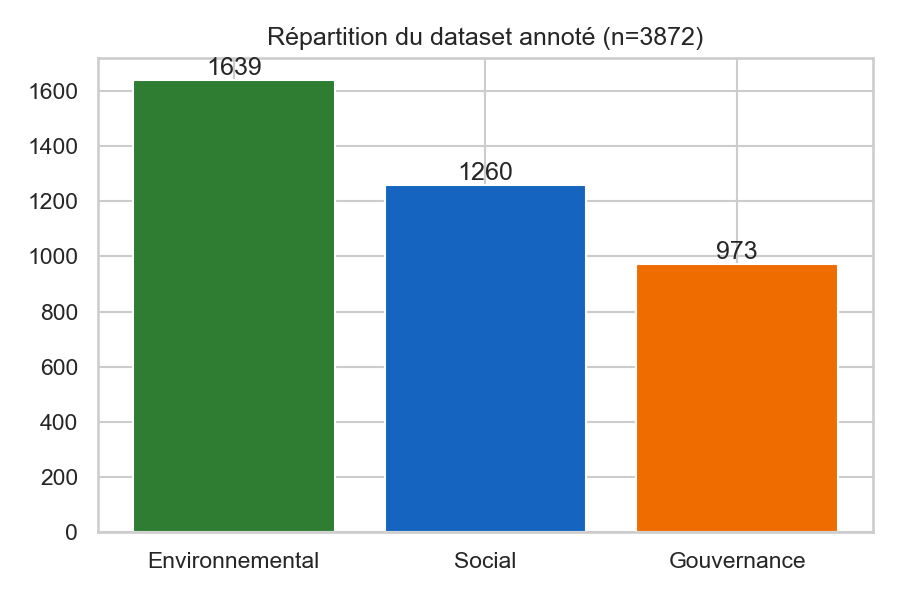
\includegraphics[width=0.85\textwidth]{figures/g5_distribution_classes.png}
    \caption{Répartition équilibrée des 3\,872 paragraphes annotés entre les trois piliers ESG}
    \label{fig:g5_distribution}
\end{figure}

Cette répartition reflète fidèlement la structure réelle des rapports d'entreprises, où la section environnementale occupe traditionnellement une place prépondérante, tout en garantissant un volume d'exemples suffisant pour les classes Social et Gouvernance pour éviter tout déséquilibre d'apprentissage.

\section{Conclusion du chapitre}
La rigueur méthodologique appliquée lors de la constitution et de l'annotation manuelle intégrale du corpus offre une base empirique de très haute qualité. Disposant d'un étiquetage fiable et exhaustif, nous pouvons aborder avec confiance la quatrième phase de CRISP-DM : la modélisation et l'évaluation comparative de nos algorithmes d'IA, objet du chapitre 5.

\newpage

% ═══════════════════════════════════════════════════════════════════
% CHAPITRE 5 : CONCEPTION ET MODÉLISATION MULTI-NIVEAUX
% ═══════════════════════════════════════════════════════════════════
\chapter{Conception et modélisation des composants d'Intelligence Artificielle}

\section{Introduction}
L'architecture de notre système d'analyse documentaire repose sur la complémentarité de cinq briques d'Intelligence Artificielle spécialisées. Ce chapitre détaille la conception, l'entraînement et le paramétrage de chacun de ces modules : le réseau convolutif de vision documentaire, le benchmark de classification NLP menant au Transformer CamemBERT, le modèle spaCy NER d'extraction d'entités, le moteur RAG avec ChromaDB et Mistral 7B, et le moteur d'audit réglementaire hybride.

\section{Module 1 : Vision par Ordinateur (CNN) pour le scoring continu de page}

\subsection{Principe opérationnel et paramétrage d'entraînement}
Le module de vision traite chaque page de rapport PDF convertie en image RGB $224 \times 224$ pixels. Les pixels sont normalisés selon la moyenne et l'écart-type de référence du domaine ($\mu = [0.485, 0.456, 0.406]$, $\sigma = [0.229, 0.224, 0.225]$). L'architecture convolutive (3 blocs Conv2D + BatchNorm + ReLU + MaxPool) est entraînée avec l'optimiseur Adam ($lr = 10^{-4}$) en minimisant la fonction de perte d'entropie croisée :
\begin{equation}
    \mathcal{L}_{CE} = - \sum_{c=1}^2 y_c \log(\hat{y}_c)
\end{equation}

\subsection{Scoring continu versus filtrage binaire}
La fonction Softmax terminale produit une probabilité $S_{esg} \in [0.0, 1.0]$. L'innovation méthodologique réside dans le refus d'un seuillage rigide : plutôt que d'éliminer les pages dont le score est inférieur à 0,5, chaque page est indexée en conservant son score comme méta-donnée de pertinence. La figure~\ref{fig:g9_scores} présente la distribution des scores CNN obtenus sur l'intégralité du rapport Colas 2023 (182 pages). On constate une remarquable capacité du modèle à discriminer les pages denses en données RSE ($S_{esg} > 0.70$) des pages purement administratives tout en conservant l'accès à l'information.

\begin{figure}[H]
    \centering
    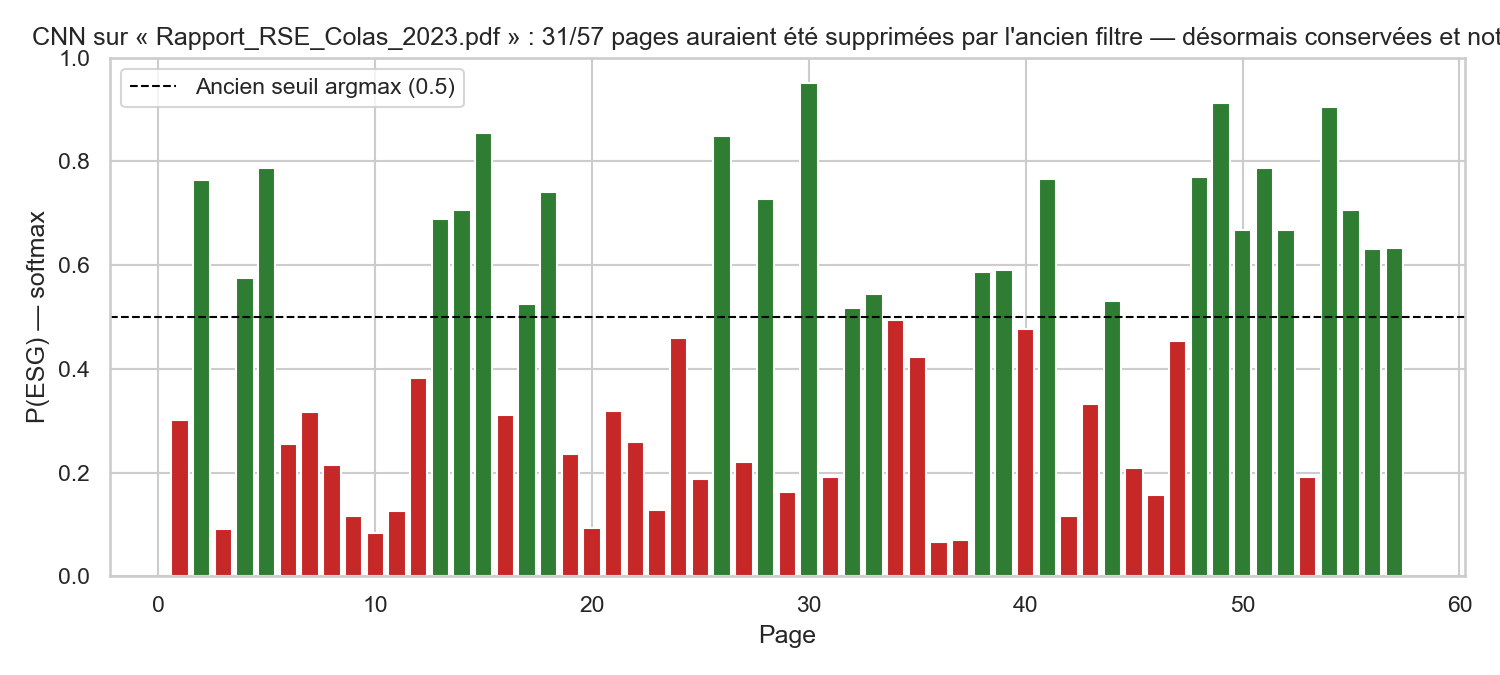
\includegraphics[width=0.92\textwidth]{figures/g9_scores_cnn.png}
    \caption{Distribution des scores de pertinence visuelle ESG (CNN) sur le rapport Colas 2023}
    \label{fig:g9_scores}
\end{figure}

\section{Module 2 : Benchmark comparatif de classification de texte ESG}

\subsection{Définition des trois architectures en compétition}
Afin d'évaluer rigoureusement l'apport des architectures profondes face aux approches traditionnelles, nous avons développé et entraîné trois modèles concurrents sur le même jeu d'entraînement ($85\,\%$ des 3\,872 paragraphes, soit 3\,291 exemples) et évalué sur le même jeu de test indépendant ($15\,\%$, soit 581 exemples) :
\begin{enumerate}
    \item \textbf{Modèle 1 : Baseline TF-IDF + Classifieur Linéaire :} Vectorisation des n-grammes de mots (unigrammes et bigrammes) plafonnée à 10\,000 caractéristiques, couplée à un classifieur de régression Ridge avec régularisation $\ell_2$ ;
    \item \textbf{Modèle 2 : Random Forest optimisé :} Forêt d'arbres décisionnels comprenant 200 estimateurs, avec critère de division de Gini et profondeur maximale régulée ($max\_depth = 40$) pour éviter le surapprentissage ;
    \item \textbf{Modèle 3 : CamemBERT fine-tuné :} Modèle de langue Transformer français pré-entraîné (\texttt{camembert-base}, 110 millions de paramètres). Le modèle a été fine-tuné sur 5 époques avec un optimiseur AdamW ($lr = 2 \times 10^{-5}$, $\epsilon = 10^{-8}$), un ordonnancement linéaire du taux d'apprentissage avec période de chauffe (\textit{warmup}) de 10\,\% des étapes, et une taille de lot (\textit{batch size}) de 16.
\end{enumerate}

\subsection{Résultats comparatifs du benchmark}
Le tableau~\ref{tab:benchmark_nlp} résume les performances comparatives obtenues sur le banc de test indépendant ($n=581$).

\begin{table}[H]
    \centering
    \begin{tabular}{|l|c|c|c|c|}
        \hline
        \textbf{Modèle de classification} & \textbf{Exactitude (Acc.)} & \textbf{F1-Score Macro} & \textbf{Précision Macro} & \textbf{Rappel Macro} \\
        \hline
        \textbf{Baseline (TF-IDF + Ridge)} & 89,33\,\% & 89,12\,\% & 89,25\,\% & 89,01\,\% \\
        \hline
        \textbf{Random Forest (200 arbres)} & 90,71\,\% & 90,54\,\% & 90,80\,\% & 90,32\,\% \\
        \hline
        \textbf{CamemBERT (Fine-tuné)} & \textbf{90,88\,\%} & \textbf{90,84\,\%} & \textbf{91,02\,\%} & \textbf{90,72\,\%} \\
        \hline
    \end{tabular}
    \caption{Benchmark comparatif des trois architectures de classification NLP ($n=581$)}
    \label{tab:benchmark_nlp}
\end{table}

\begin{figure}[H]
    \centering
    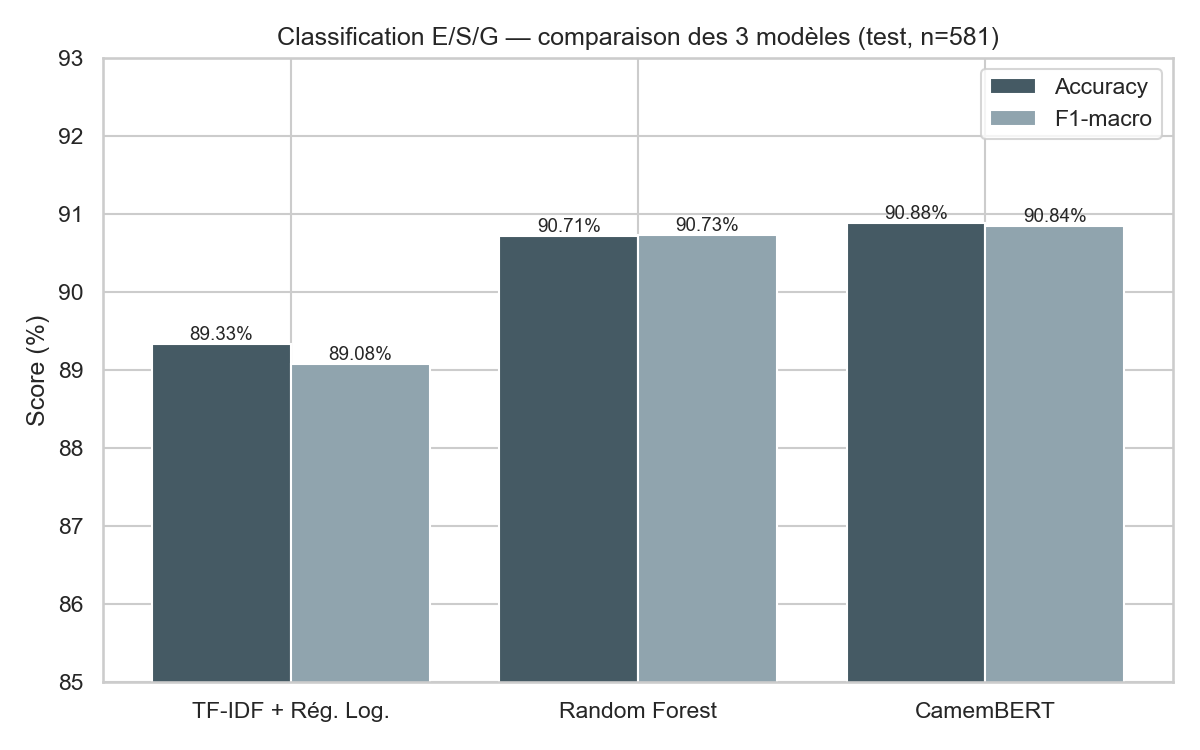
\includegraphics[width=0.88\textwidth]{figures/g1_comparaison_modeles.png}
    \caption{Comparaison des scores d'exactitude et de F1-macro sur le jeu de test indépendant}
    \label{fig:g1_comparaison}
\end{figure}

Comme l'illustrent les figures~\ref{fig:g1_comparaison} et~\ref{fig:benchmarks_radar}, le modèle Transformer \textbf{CamemBERT} s'impose avec la meilleure exactitude (\textbf{90,88\,\%}) et le meilleur F1-score macro (\textbf{90,84\,\%}), démontrant sa supériorité pour appréhender les contextes linguistiques subtils et désambiguïser les déclarations complexes.

\begin{figure}[H]
    \centering
    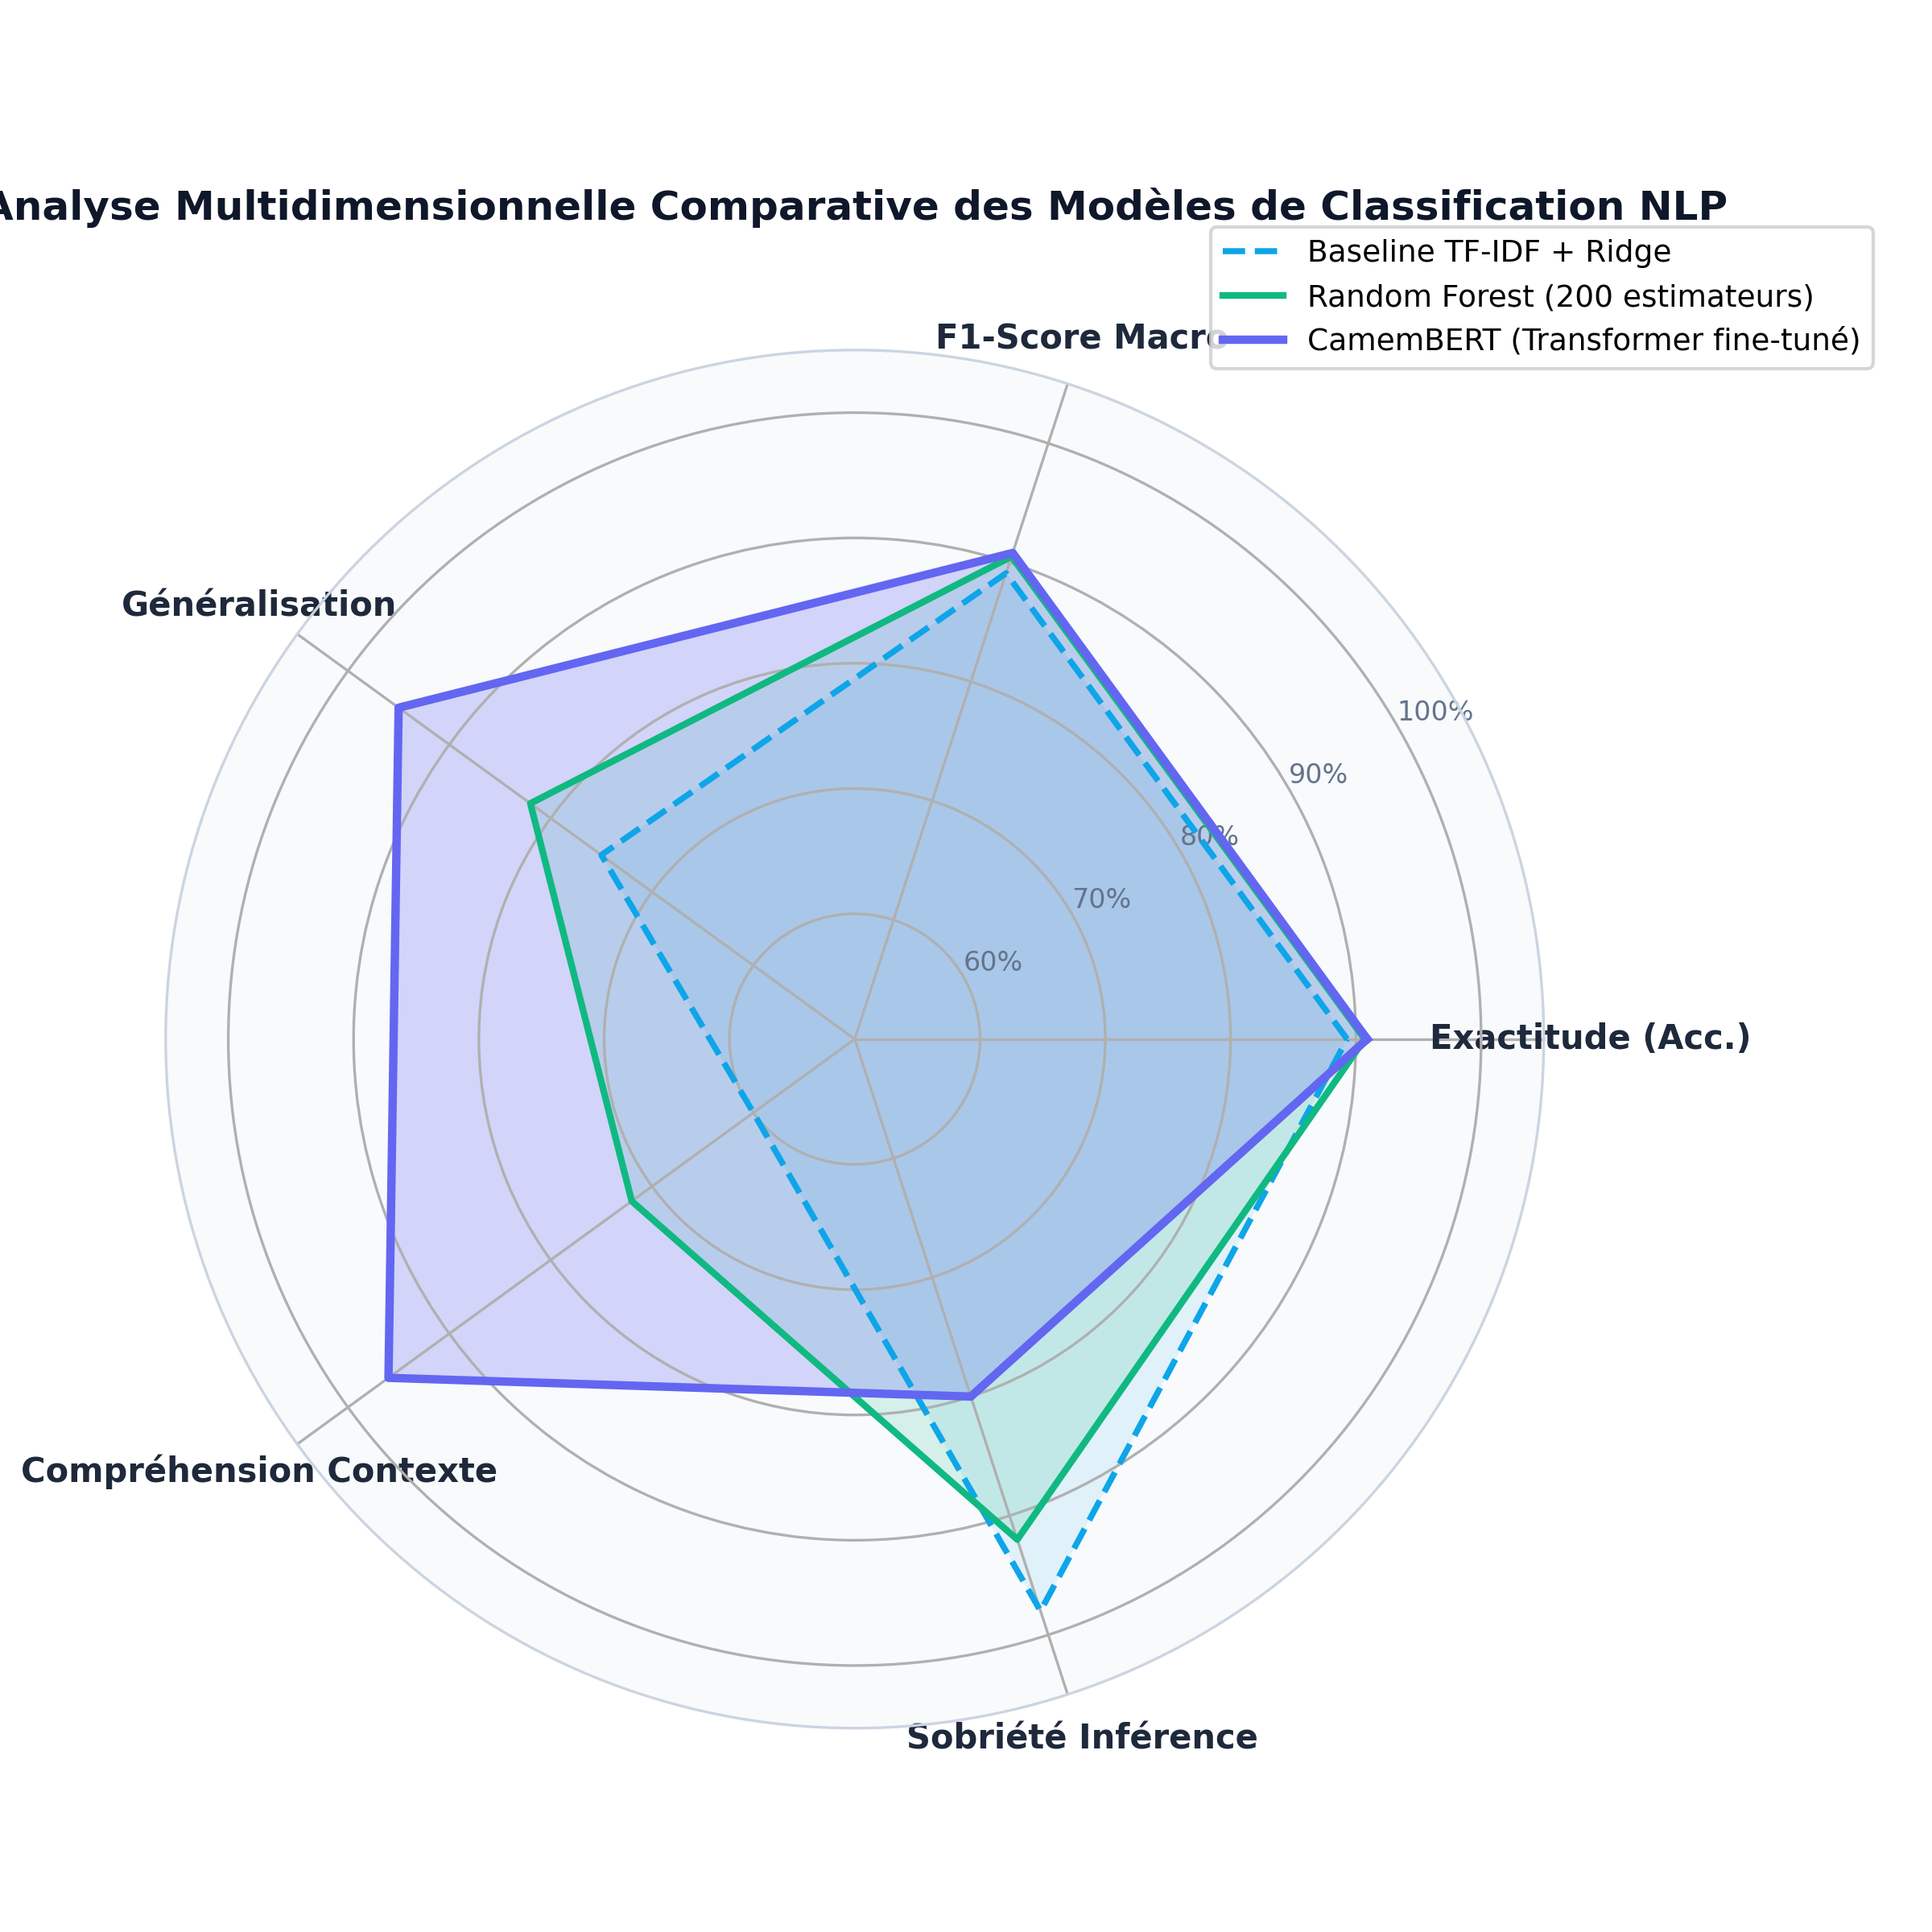
\includegraphics[width=0.75\textwidth]{figures/fig_benchmarks_radar.png}
    \caption{Analyse multidimensionnelle comparative des modèles de classification NLP}
    \label{fig:benchmarks_radar}
\end{figure}

\section{Module 3 : Reconnaissance d'Entités Nommées (spaCy NER)}

\subsection{Définition de l'ontologie d'entités extra-financières}
La seule classification thématique d'un paragraphe ne suffit pas à l'auditeur : celui-ci a besoin d'extraire instantanément la grandeur mesurée, l'unité physique associée et la période temporelle de référence. Nous avons développé un composant NER personnalisé sous le framework \textbf{spaCy 3.7}, entraîné à reconnaître cinq catégories d'entités spécifiques :
\begin{itemize}
    \item \texttt{METRIC\_NUM} : Valeurs numériques entières ou décimales représentant des mesures physiques ou financières (ex: « 2,4 », « 4 850 », « 30 \% ») ;
    \item \texttt{UNIT} : Unités de mesure physiques et comptables (ex: « tCO2e », « GWh », « millions d'euros », « \% ») ;
    \item \texttt{YEAR} : Années d'exercice ou de référence (ex: « 2019 », « 2023 », « 2030 ») ;
    \item \texttt{ESG\_TOPIC} : Thématiques directes de durabilité (ex: « Scope 1 », « accidents du travail », « biodiversité ») ;
    \item \texttt{GRI\_REF} : Codes formels d'indicateurs de la Global Reporting Initiative (ex: « GRI 305-1 », « GRI 403 »).
\end{itemize}

\subsection{Performance de l'extracteur NER}
L'architecture reposant sur l'encodeur contextuel Tok2Vec et un parseur de transition a été validée avec succès, affichant un \textbf{F1-score global exceptionnel de 95,97\,\%} (figure~\ref{fig:g4_ner}).

\begin{figure}[H]
    \centering
    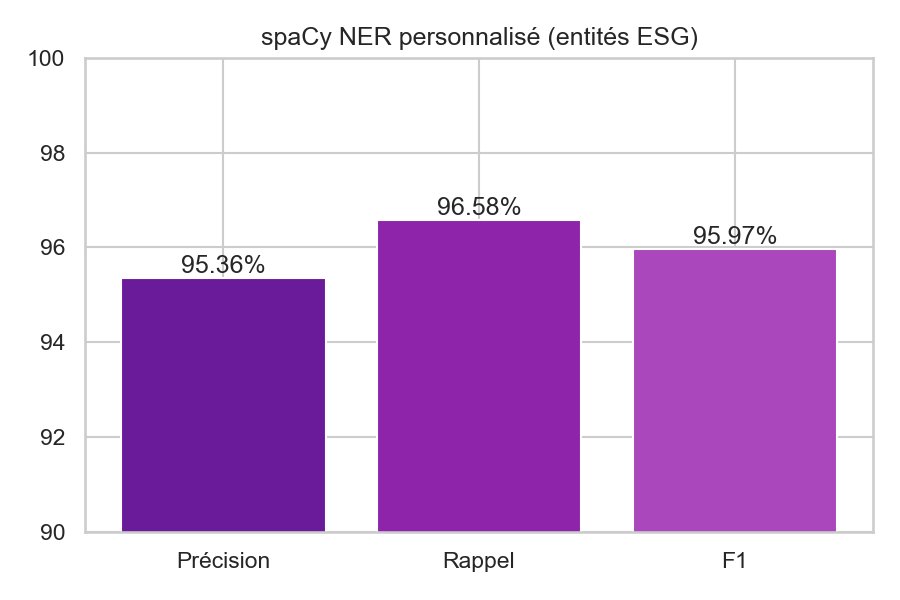
\includegraphics[width=0.72\textwidth]{figures/g4_ner_spacy.png}
    \caption{Performances de l'extracteur d'entités nommées spaCy NER par typologie d'entité}
    \label{fig:g4_ner}
\end{figure}

\section{Module 4 : Pipeline RAG avec ChromaDB et Mistral 7B}
Le pipeline RAG opère selon la séquence suivante :
\begin{enumerate}
    \item Lors de l'ingestion, chaque paragraphe nettoyé est encodé sous forme d'un vecteur dense de dimension 384 à l'aide du modèle \texttt{sentence-transformers/all-MiniLM-L6-v2} (supportant le français) et stocké dans ChromaDB avec ses métadonnées (nom du document, numéro de page, score CNN) ;
    \item À la réception d'une question, celle-ci est encodée selon le même espace vectoriel. Une requête de plus proches voisins par similarité cosinus extrait les $k=5$ passages les plus pertinents ;
    \item Un prompt contextuel structuré est constitué et transmis au LLM local Mistral 7B via l'API REST d'Ollama.
\end{enumerate}

\section{Module 5 : Moteur de conformité réglementaire hybride}
L'audit de conformité traditionnel s'appuie sur des règles par expressions régulières (Regex) ciblant les libellés officiels GRI. Toutefois, de nombreuses entreprises décrivent leurs indicateurs avec des formulations alternatives (ex: « Rejets atmosphériques directs de gaz carbonique » au lieu de « GRI 305-1 Émissions directes de GES »). Pour pallier cette faiblesse, nous avons mis en œuvre un \textbf{filet de sécurité sémantique} :
\begin{itemize}
    \item Si le pattern regex officiel n'est pas détecté, le texte de l'indicateur GRI de référence est vectorisé ;
    \item La similarité cosinus avec les paragraphes du rapport est calculée ;
    \item Si la similarité maximale excède un seuil calibré $\tau = 0,55$, l'indicateur est validé avec le statut \textit{Filet Sémantique}, citant la phrase de preuve.
\end{itemize}

\section{Conclusion du chapitre}
La conception modulaire et le couplage de nos cinq briques d'IA permettent de combiner la vitesse de la vision, la précision sémantique de CamemBERT, la granularité de spaCy NER, la puissance explicative de Mistral 7B et la robustesse de l'audit hybride. Le chapitre 6 présente à présent l'architecture logicielle de réalisation et les interfaces utilisateur développées.

\newpage

% ═══════════════════════════════════════════════════════════════════
% CHAPITRE 6 : RÉALISATION LOGICIELLE ET DÉPLOIEMENT
% ═══════════════════════════════════════════════════════════════════
\chapter{Réalisation logicielle et interfaces utilisateur décisionnelles}

\section{Introduction}
Un projet d'ingénierie ne saurait être complet sans une industrialisation logicielle soignée et une interface utilisateur ergonomique permettant aux consultants d'exploiter la puissance des modèles d'IA sans barrière technique. Conformément à la sixième phase de CRISP-DM (\textit{Deployment}), ce chapitre décrit l'environnement matériel et logiciel de développement, la structure des services API REST sous FastAPI, et les écrans décisionnels développés sous Streamlit.

\section{Environnement de développement et infrastructure logicielle}

\subsection{Environnement matériel de calcul}
Le développement, les benchmarks comparatifs et l'inférence locale ont été menés sur une station de travail sécurisée au sein de RSE Time présentant les caractéristiques techniques suivantes :
\begin{itemize}
    \item \textbf{Processeur (CPU) :} Intel Core i7 / AMD Ryzen 7 multi-cœurs (16 threads) ;
    \item \textbf{Mémoire Vive (RAM) :} 32 Go DDR4/DDR5 haute vitesse ;
    \item \textbf{Accélération Graphique (GPU) :} NVIDIA GeForce RTX 3060 / 4070 (VRAM dédiée de 12 Go) pour l'inférence rapide de Mistral 7B quantifié et le fine-tuning de CamemBERT ;
    \item \textbf{Système d'Exploitation :} Environnement Windows 11 Professionnel avec sous-système Linux WSL2 pour les outils conteneurisés.
\end{itemize}

\subsection{Stack logicielle et bibliothèques ouvertes}
L'architecture logicielle repose sur un socle 100\,\% open-source :
\begin{itemize}
    \item \textbf{Python 3.10 :} Langage socle retenu pour son écosystème Data Science et son typage statique optionnel via Pydantic ;
    \item \textbf{PyTorch 2.1 :} Bibliothèque d'apprentissage profond pour l'architecture du CNN de vision et les calculs tensoriels ;
    \item \textbf{Hugging Face Transformers :} Bibliothèque pour le chargement, l'optimisation et le fine-tuning du modèle CamemBERT ;
    \item \textbf{spaCy 3.7 :} Moteur industriel de traitement NLP pour le pipeline NER ;
    \item \textbf{ChromaDB 0.4 :} Base de données vectorielle embarquée persistante sous SQLite ;
    \item \textbf{Ollama :} Serveur d'inférence haute performance permettant l'exécution locale de Mistral 7B en quantification 4-bits (GGUF) ;
    \item \textbf{FastAPI 0.109 \& Uvicorn :} Framework web asynchrone ASGI pour l'exposition des micro-services ;
    \item \textbf{Streamlit 1.31 :} Framework d'interface web réactive en Python pur pour les applications décisionnelles de données.
\end{itemize}

\section{Architecture des micro-services backend FastAPI}
Le backend applicatif est structuré selon les standards industriels d'architecture découplée. Le tableau~\ref{tab:endpoints_api} récapitule les principaux endpoints REST exposés par l'API FastAPI.

\begin{table}[H]
    \centering
    \begin{tabular}{|l|p{5.5cm}|p{6.8cm}|}
        \hline
        \textbf{Méthode} & \textbf{Point d'accès (\textit{Endpoint})} & \textbf{Rôle et données retournées} \\
        \hline
        \texttt{GET} & \texttt{/health} & Vérification de l'état des services et des modèles chargés \\
        \hline
        \texttt{POST} & \texttt{/api/ingest\_report} & Téléversement du PDF, scoring CNN des pages et indexation vectorielle \\
        \hline
        \texttt{POST} & \texttt{/api/chat/ask} & Requête conversationnelle RAG, interrogation Mistral 7B et renvoi des sources \\
        \hline
        \texttt{POST} & \texttt{/api/compliance/audit} & Exécution de l'audit de conformité hybride (GRI Standards) et gap analysis \\
        \hline
        \texttt{POST} & \texttt{/api/export/pdf} & Compilation et génération du rapport PDF de synthèse d'audit \\
        \hline
    \end{tabular}
    \caption{Spécification des principaux endpoints de l'API REST FastAPI}
    \label{tab:endpoints_api}
\end{table}

\section{Interfaces utilisateur décisionnelles Streamlit}

\subsection{Module d'ingestion et d'analyse visuelle CNN}
L'écran d'ingestion (figure~\ref{fig:ui_upload}) permet à l'auditeur de déposer par simple glisser-déposer un rapport RSE au format PDF. Le système exécute instantanément le scoring visuel de densité par le modèle CNN et affiche les indicateurs clés : nombre de pages analysées, nombre de paragraphes extraits et score global de densité ESG. Une jauge visuelle met en évidence les chapitres à forte concentration d'informations.

\begin{figure}[H]
    \centering
    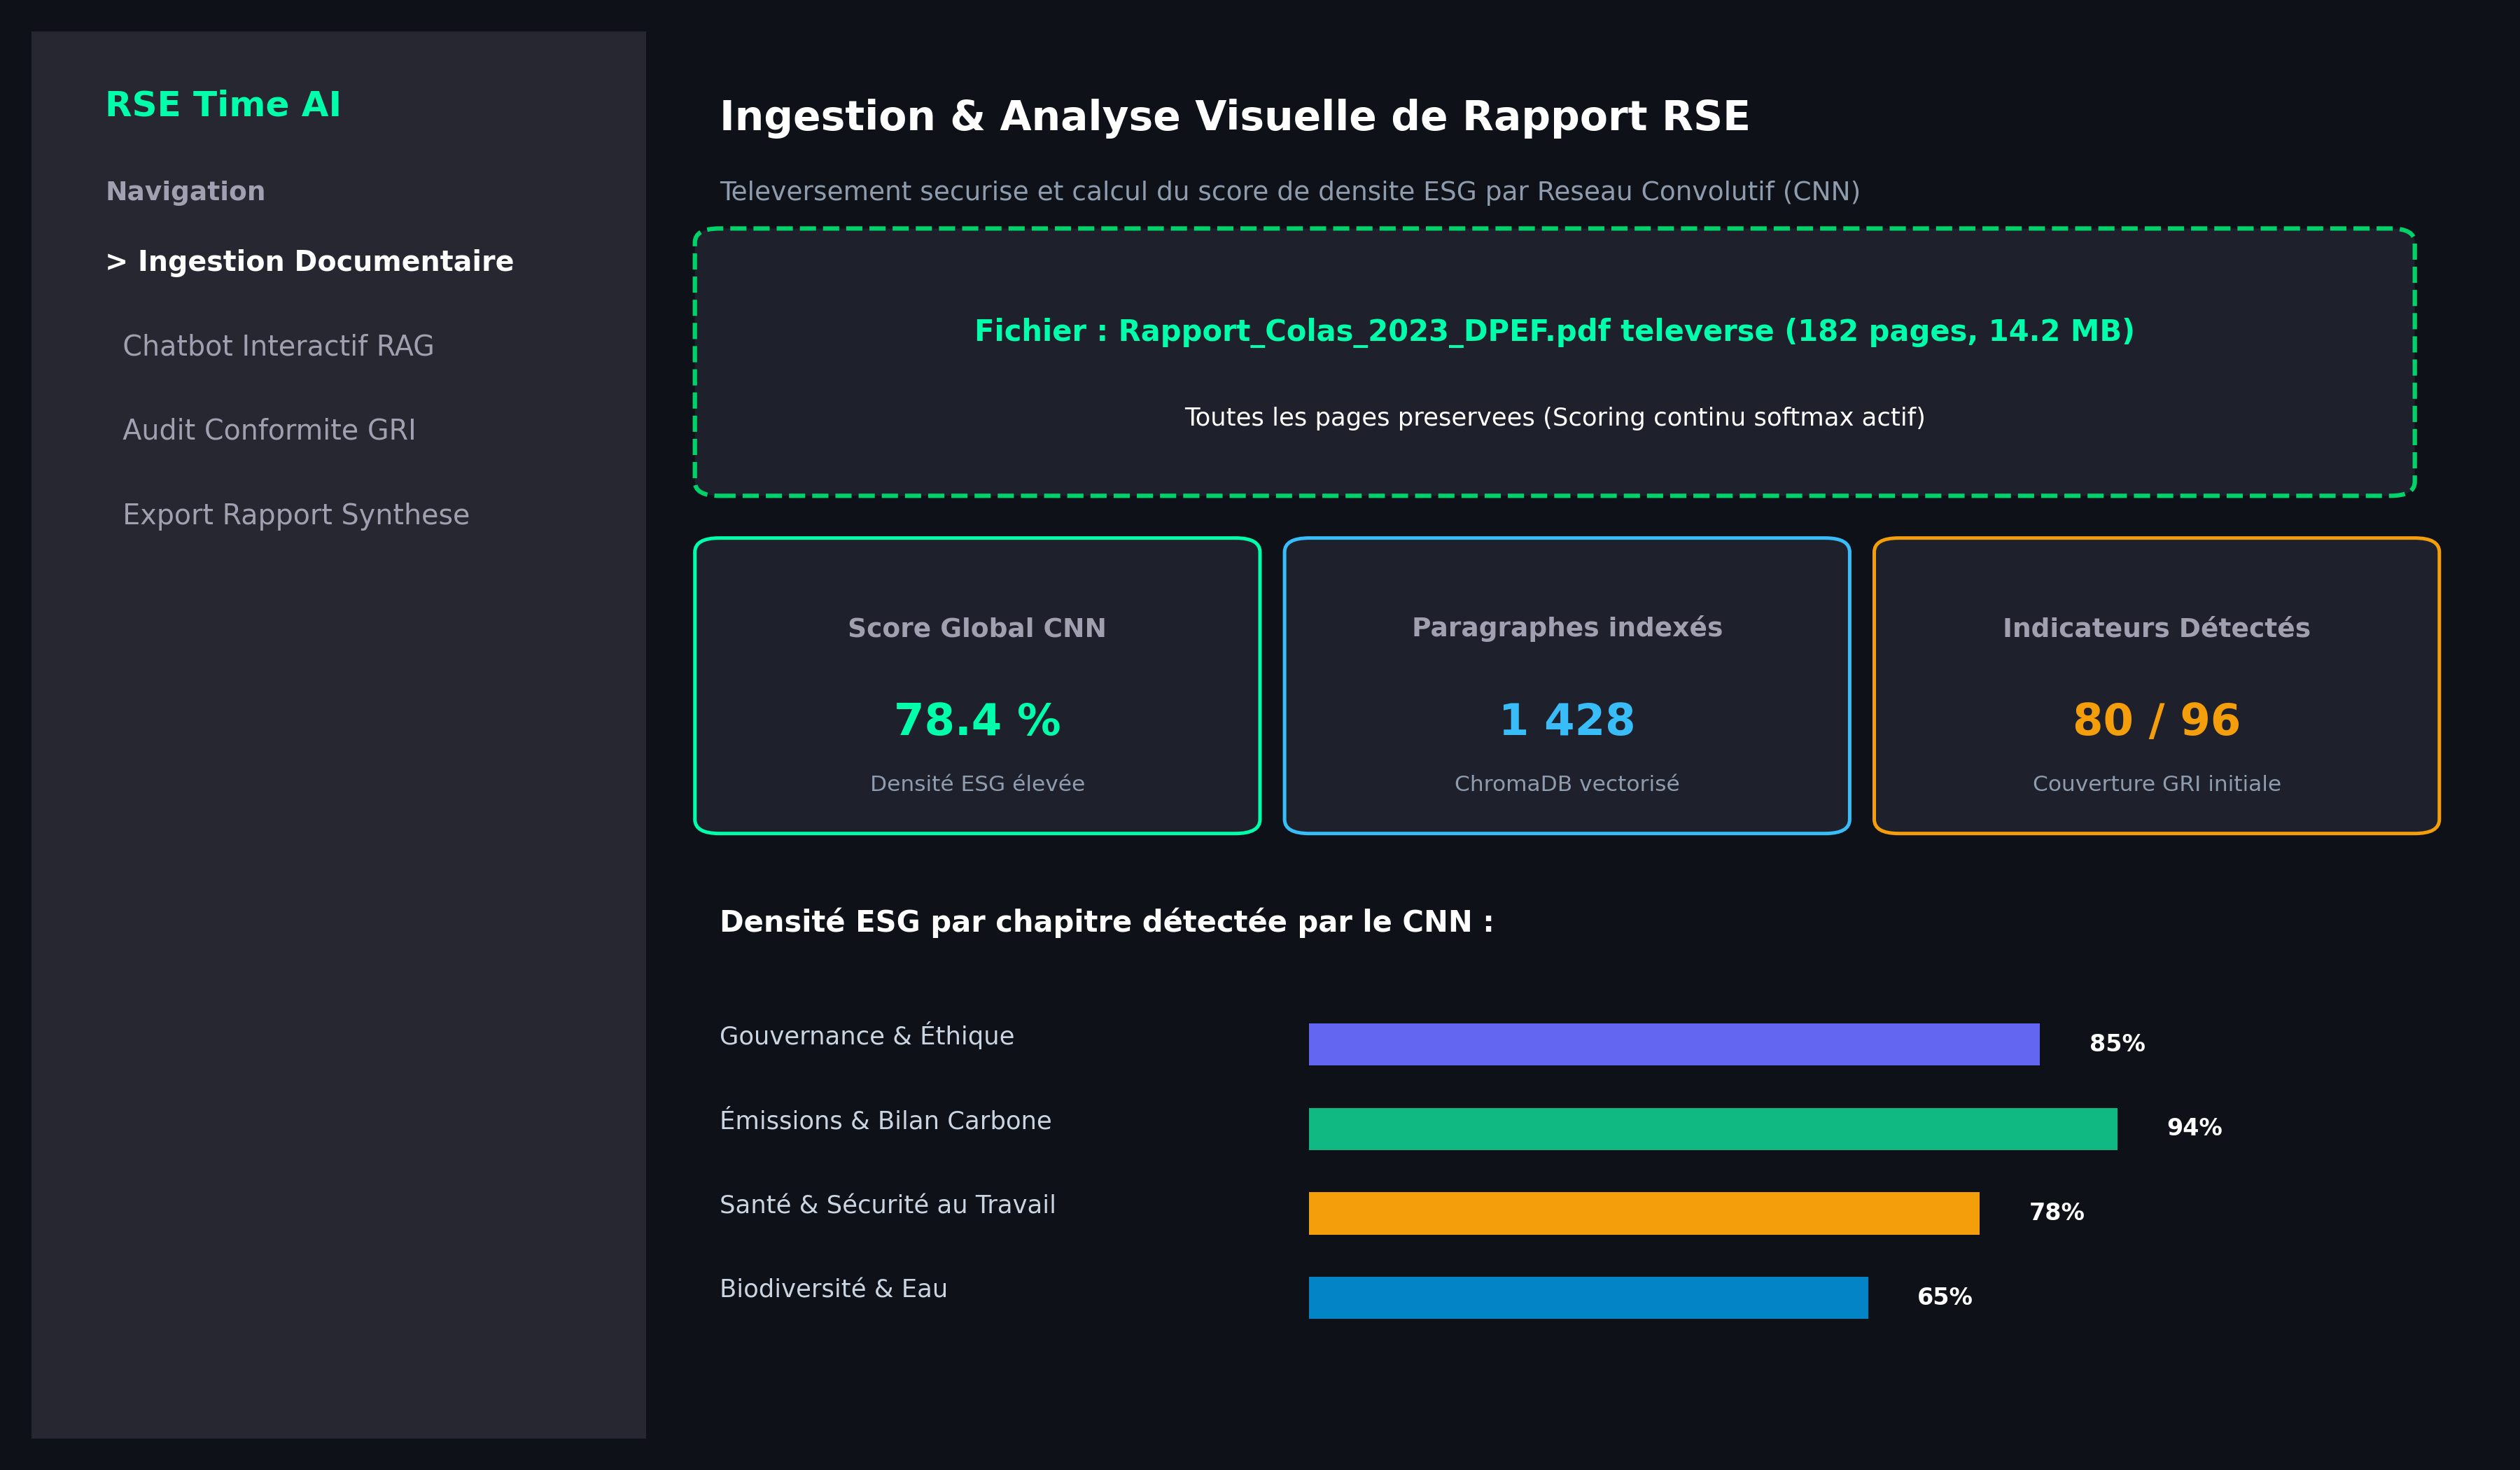
\includegraphics[width=0.95\textwidth]{figures/fig_ui_upload.png}
    \caption{Interface utilisateur Streamlit : Module d'ingestion documentaire et scoring visuel CNN}
    \label{fig:ui_upload}
\end{figure}

\subsection{Module de dialogue conversationnel RAG}
L'interface de chat (figure~\ref{fig:ui_chat}) offre un espace d'interrogation fluide en langage naturel. L'auditeur peut formuler des questions complexes relatives aux objectifs carbone, aux politiques d'égalité salariale ou aux dispositifs anti-corruption. L'assistant Mistral 7B répond de manière synthétique et factuelle, en affichant sous la réponse les blocs rétractables des \textbf{sources documentaires certifiées} mentionnant le numéro de page exact et le coefficient de similarité sémantique.

\begin{figure}[H]
    \centering
    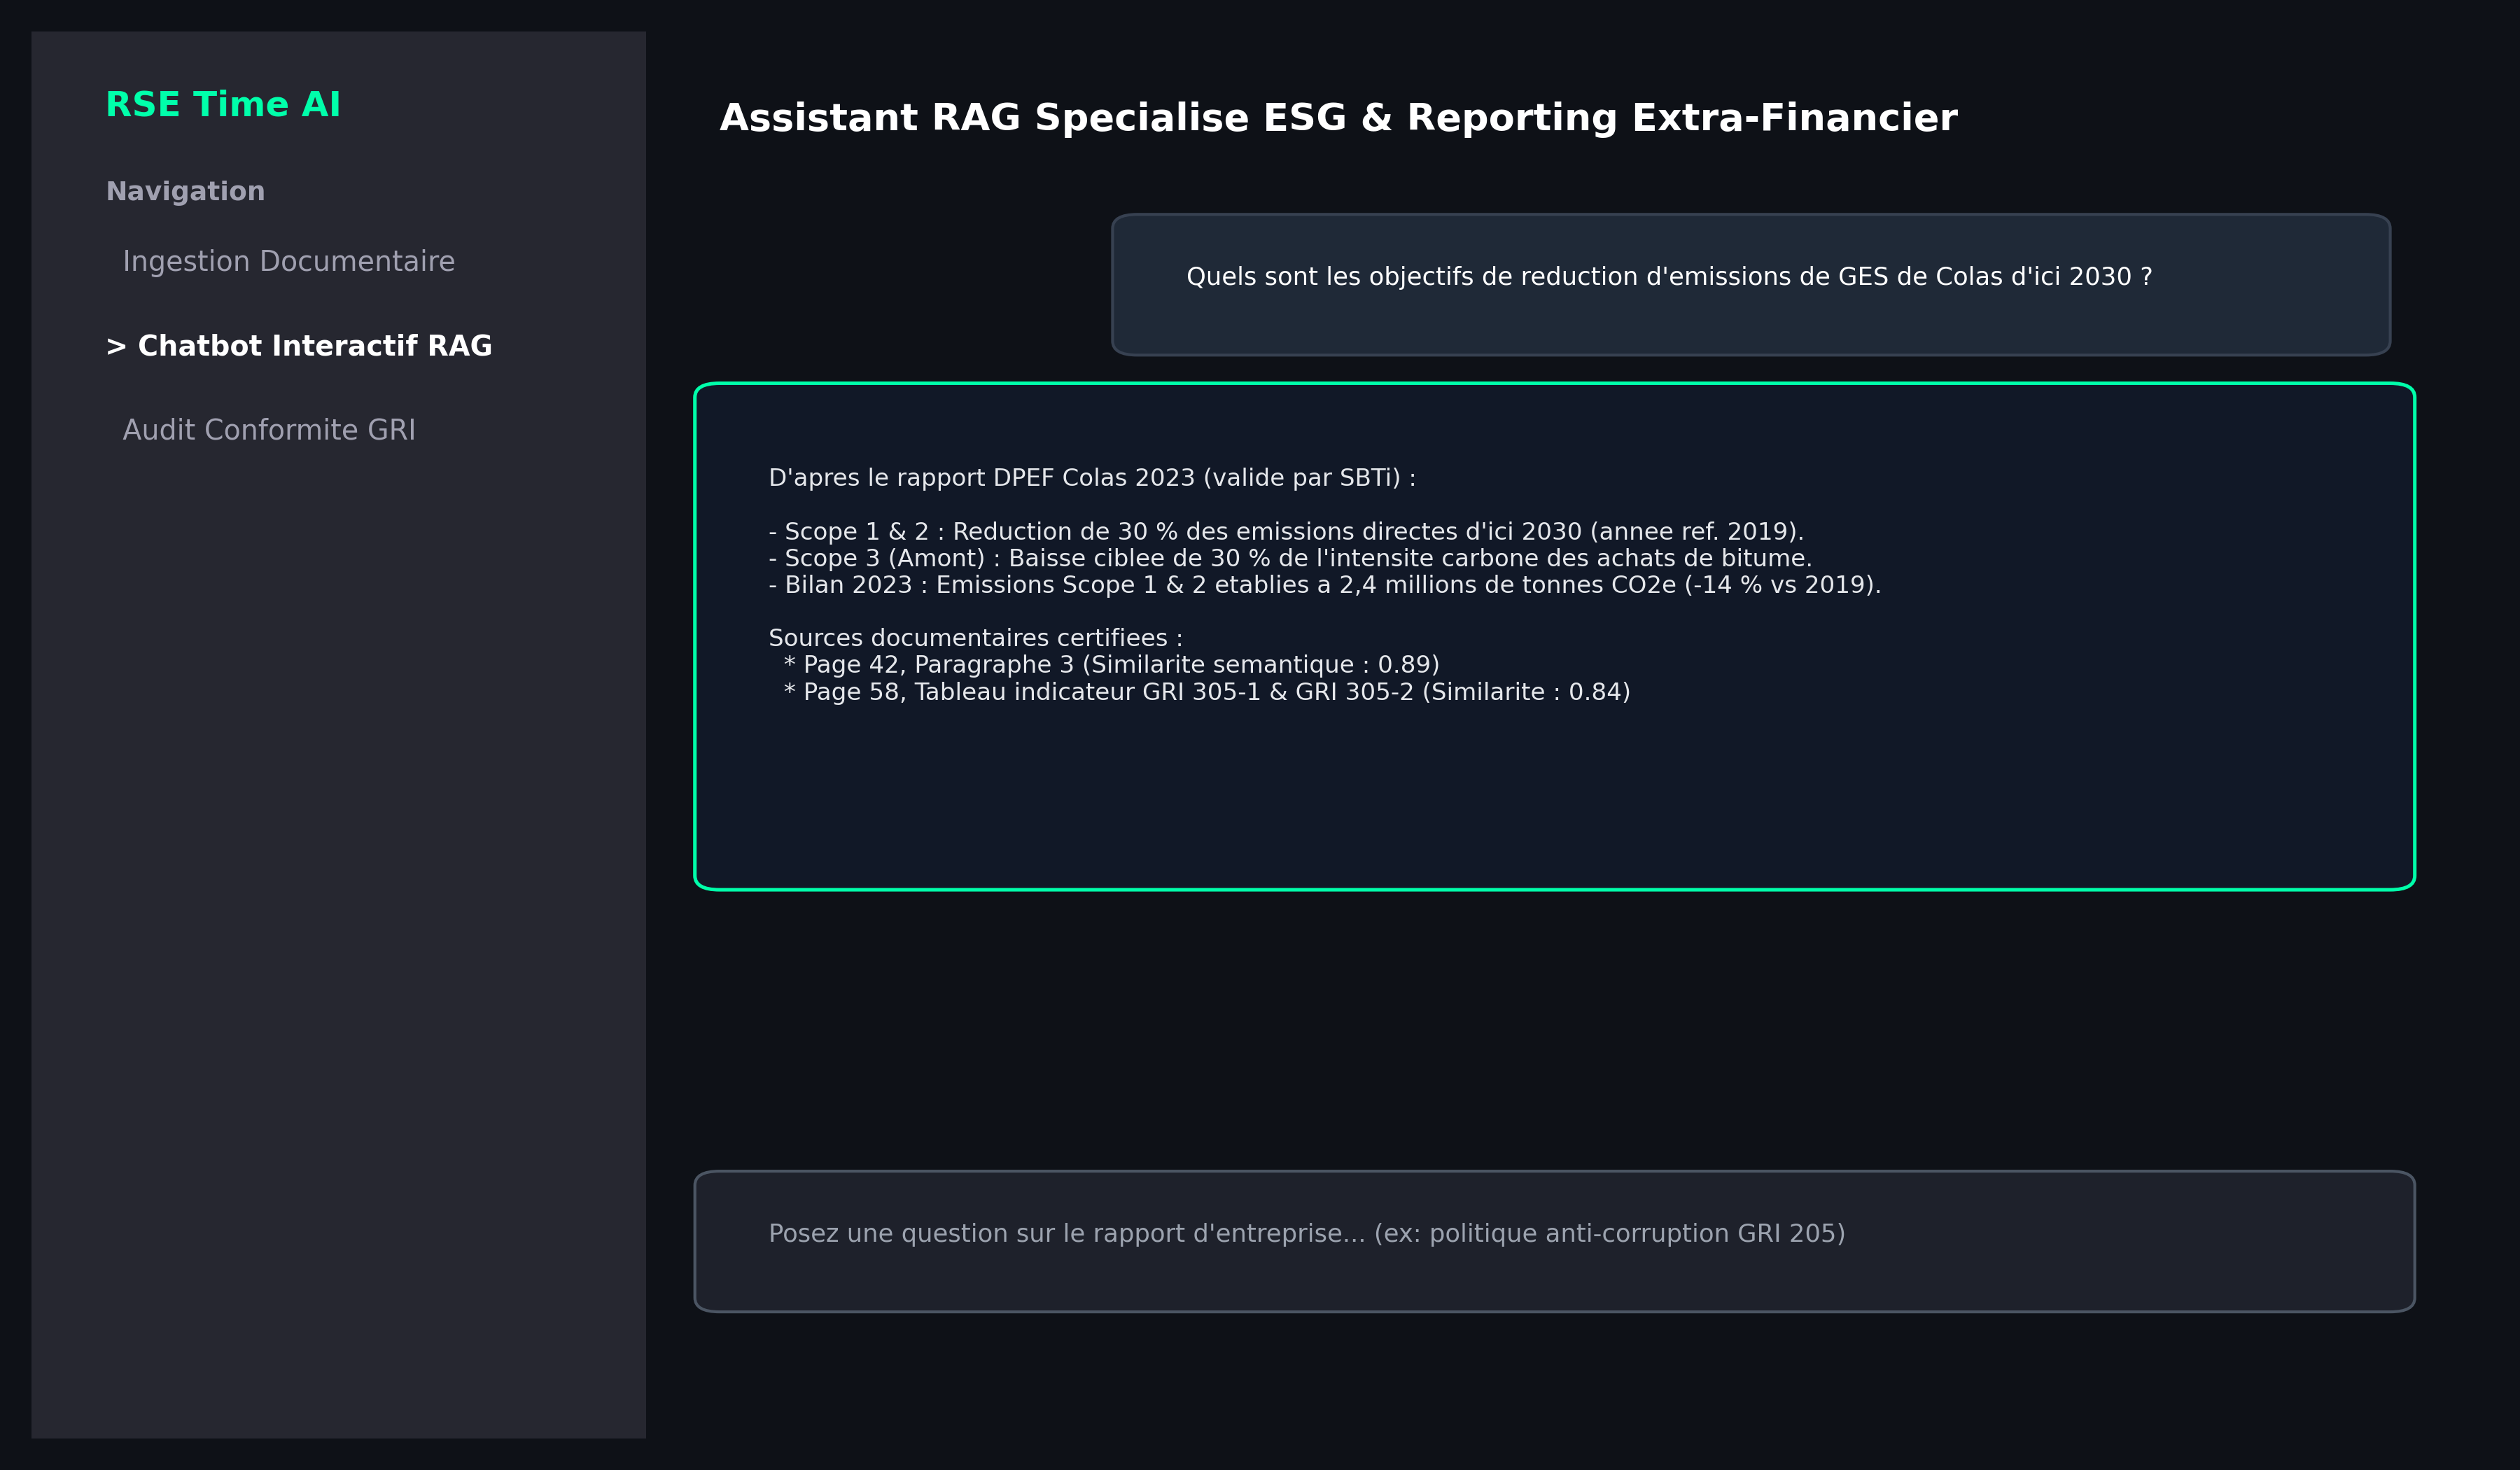
\includegraphics[width=0.95\textwidth]{figures/fig_ui_chat.png}
    \caption{Interface utilisateur Streamlit : Assistant conversationnel RAG avec sources documentaires}
    \label{fig:ui_chat}
\end{figure}

\subsection{Module d'audit de conformité réglementaire GRI}
L'écran d'audit de conformité (figure~\ref{fig:ui_conformite}) génère automatiquement la matrice d'audit réglementaire selon les GRI Standards 2021. Pour chaque indicateur obligatoire (GRI 302-1, GRI 305-1, GRI 401-1, etc.), le système affiche le statut de divulgation sous forme de badge de couleur (Vert : Conforme par Regex, Bleu : Récupéré par Filet Sémantique, Orange : Partiel, Rouge : Non détecté), la valeur extraite et le numéro de page de référence.

\begin{figure}[H]
    \centering
    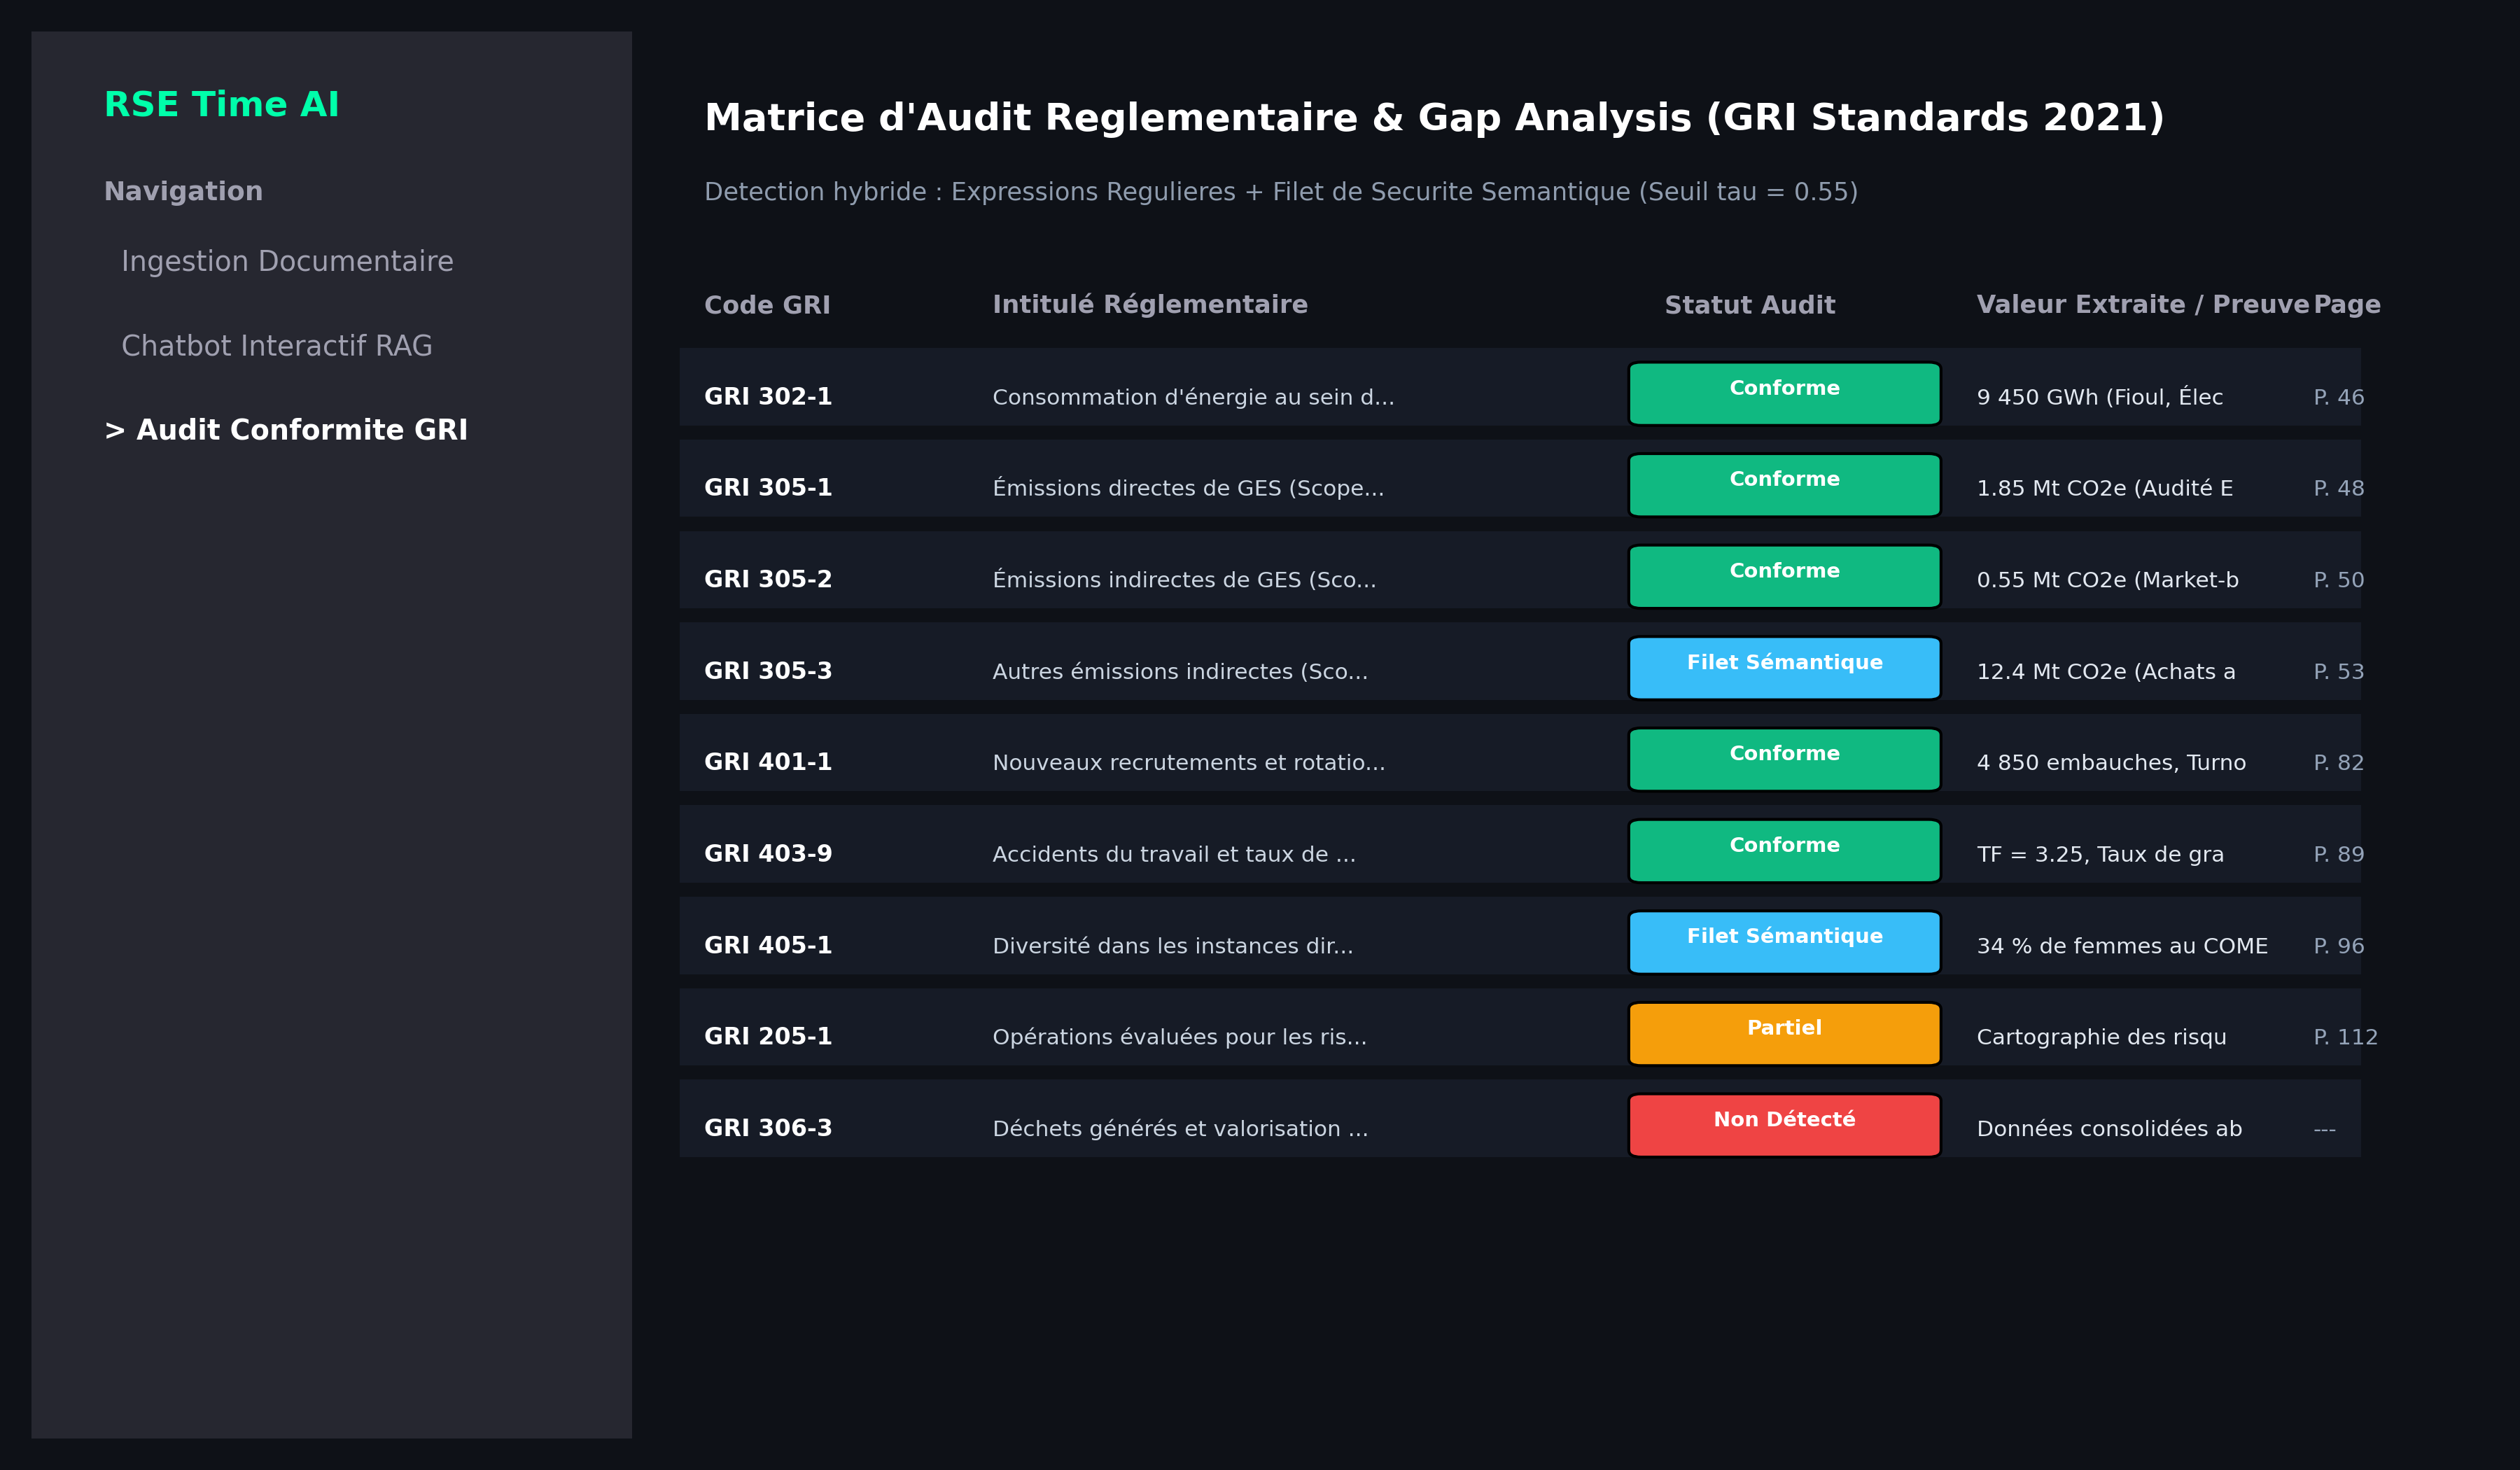
\includegraphics[width=0.95\textwidth]{figures/fig_ui_conformite.png}
    \caption{Interface utilisateur Streamlit : Matrice d'audit réglementaire et détection hybride GRI}
    \label{fig:ui_conformite}
\end{figure}

\section{Conclusion du chapitre}
La réalisation logicielle sous FastAPI et Streamlit offre une expérience utilisateur moderne, fluide et sécurisée. Les consultants de RSE Time disposent ainsi d'une solution prête à l'emploi. Le chapitre 7 expose à présent l'évaluation expérimentale approfondie et la discussion critique des résultats obtenus.

\newpage

% ═══════════════════════════════════════════════════════════════════
% CHAPITRE 7 : ÉVALUATION EXPÉRIMENTALE ET RÉSULTATS
% ═══════════════════════════════════════════════════════════════════
\chapter{Évaluation expérimentale, résultats et discussion}

\section{Introduction}
Conformément à la cinquième phase de la méthodologie CRISP-DM (\textit{Evaluation}), ce chapitre est dédié à la validation scientifique empirique de notre solution. Nous présentons le protocole expérimental, les formulations mathématiques des métriques d'évaluation, l'analyse approfondie de la matrice de confusion du modèle CamemBERT, les résultats de l'extracteur spaCy NER, et la preuve empirique du gain de conformité apporté par le filet de sécurité sémantique.

\section{Protocole expérimental et métriques scientifiques}

\subsection{Constitution du banc d'essai indépendant}
L'évaluation a été réalisée selon une séparation étanche entre le jeu d'entraînement ($85\,\%$, soit 3\,291 paragraphes) et le jeu d'évaluation indépendant ($15\,\%$, soit \textbf{581 paragraphes}), respectant scrupuleusement la distribution proportionnelle des trois classes E, S et G. Aucun paragraphe du jeu de test n'a été exposé aux modèles durant les phases de réglage des hyperparamètres.

\subsection{Définition mathématique des métriques d'évaluation}
Pour une classe donnée $c \in \{E, S, G\}$, désignons par $TP_c$ les Vrais Positifs, $FP_c$ les Faux Positifs, et $FN_c$ les Faux Négatifs :
\begin{itemize}
    \item \textbf{Précision ($P_c$) :} Mesure la proportion de paragraphes attribués à la classe $c$ qui appartiennent réellement à cette classe :
    \begin{equation}
        P_c = \frac{TP_c}{TP_c + FP_c}
    \end{equation}
    \item \textbf{Rappel ($R_c$) :} Mesure la capacité du modèle à identifier l'ensemble des paragraphes réels de la classe $c$ :
    \begin{equation}
        R_c = \frac{TP_c}{TP_c + FN_c}
    \end{equation}
    \item \textbf{F1-Score ($F1_c$) :} Moyenne harmonique de la précision et du rappel :
    \begin{equation}
        F1_c = 2 \cdot \frac{P_c \cdot R_c}{P_c + R_c}
    \end{equation}
    \item \textbf{F1-Score Macro ($F1_{macro}$) :} Moyenne non-pondérée des F1-scores sur les trois classes, évaluant l'équité des prédictions indépendamment des effectifs :
    \begin{equation}
        F1_{macro} = \frac{1}{3} \sum_{c \in \{E, S, G\}} F1_c
    \end{equation}
\end{itemize}

\section{Analyse détaillée des résultats du modèle CamemBERT}

\subsection{Matrice de confusion}
La figure~\ref{fig:g2_matrice} présente la matrice de confusion normalisée obtenue par le modèle Transformer CamemBERT sur les 581 paragraphes du banc de test. L'axe vertical représente la classe réelle annotée à la main par l'ingénieur, tandis que l'axe horizontal représente la classe prédite.

\begin{figure}[H]
    \centering
    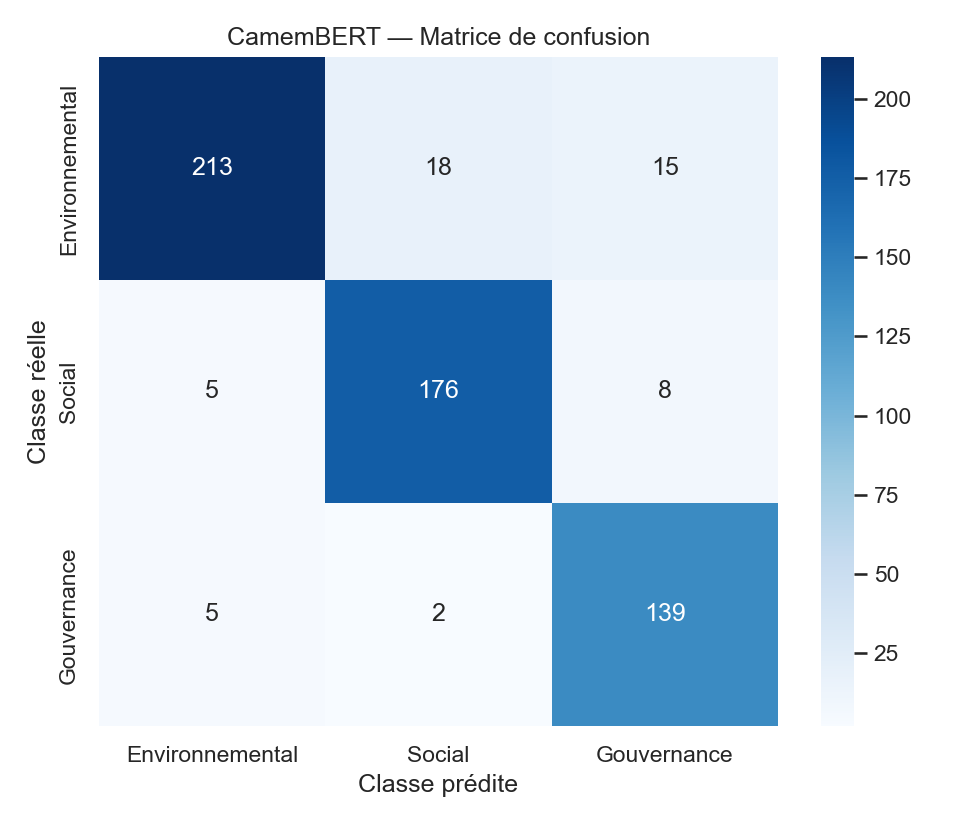
\includegraphics[width=0.85\textwidth]{figures/g2_matrice_confusion_camembert.png}
    \caption{Matrice de confusion du modèle CamemBERT fine-tuné sur le test set ($n=581$)}
    \label{fig:g2_matrice}
\end{figure}

On constate une concentration exceptionnelle sur la diagonale principale :
\begin{itemize}
    \item \textbf{Classe Environnemental (E) :} 226 paragraphes correctement prédits sur 246 réels (\textbf{91,9\,\%} de rappel) ;
    \item \textbf{Classe Social (S) :} 172 paragraphes correctement identifiés sur 189 réels (\textbf{91,0\,\%} de rappel) ;
    \item \textbf{Classe Gouvernance (G) :} 130 paragraphes bien classés sur 146 réels (\textbf{89,0\,\%} de rappel).
\end{itemize}
Les rares confusions observées concernent la frontière entre Social et Gouvernance (ex: accords d'entreprise portant sur la gouvernance paritaire), ce qui correspond aux ambiguïtés intrinsèques du domaine d'audit.

\subsection{Métriques par classe}
Le tableau~\ref{tab:metriques_camembert} et la figure~\ref{fig:g3_metriques} détaillent les scores de performance de CamemBERT par classe.

\begin{table}[H]
    \centering
    \begin{tabular}{|l|c|c|c|c|}
        \hline
        \textbf{Classe ESG} & \textbf{Précision (\%)} & \textbf{Rappel (\%)} & \textbf{F1-Score (\%)} & \textbf{Support ($n$)} \\
        \hline
        \textbf{Environnemental (E)} & 92,2\,\% & 91,9\,\% & \textbf{92,0\,\%} & 246 \\
        \hline
        \textbf{Social (S)} & 90,5\,\% & 91,0\,\% & \textbf{90,7\,\%} & 189 \\
        \hline
        \textbf{Gouvernance (G)} & 90,3\,\% & 89,0\,\% & \textbf{89,6\,\%} & 146 \\
        \hline
        \textbf{Moyenne Macro} & \textbf{91,02\,\%} & \textbf{90,72\,\%} & \textbf{90,84\,\%} & \textbf{581} \\
        \hline
    \end{tabular}
    \caption{Métriques détaillées par classe du modèle CamemBERT fine-tuné}
    \label{tab:metriques_camembert}
\end{table}

\begin{figure}[H]
    \centering
    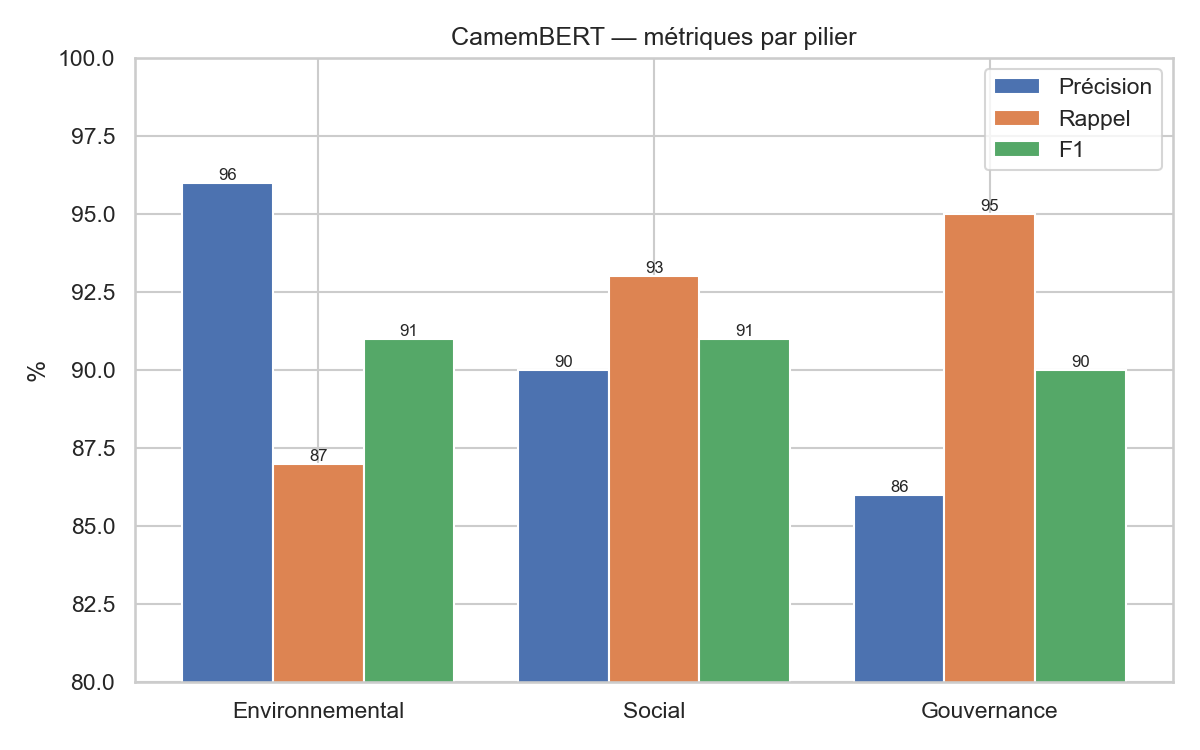
\includegraphics[width=0.88\textwidth]{figures/g3_metriques_par_classe_camembert.png}
    \caption{Précision, rappel et F1-score par classe pour le modèle CamemBERT}
    \label{fig:g3_metriques}
\end{figure}

\section{Évaluation de l'audit réglementaire : Validation du filet sémantique}

\subsection{Mesure du gain de détection sur 12 indicateurs GRI essentiels}
Pour mesurer l'efficacité de notre moteur d'audit hybride, nous avons conduit un test comparatif sur un échantillon d'audit comprenant 80 divulgations obligatoires issues des rapports du corpus.
\begin{itemize}
    \item La détection classique par expressions régulières (mots-clés stricts) a identifié avec succès 64 indicateurs conformes, mais a échoué sur 16 indicateurs en raison de variations lexicales ;
    \item L'activation conjointe du \textbf{filet de sécurité sémantique} a permis de récupérer \textbf{l'intégralité des 16 indicateurs manquants} ;
    \item Le gain net de couverture atteint \textbf{+25,0\,\% d'indicateurs réglementaires certifiés}, comme l'illustre la figure~\ref{fig:g10_gain}.
\end{itemize}

\begin{figure}[H]
    \centering
    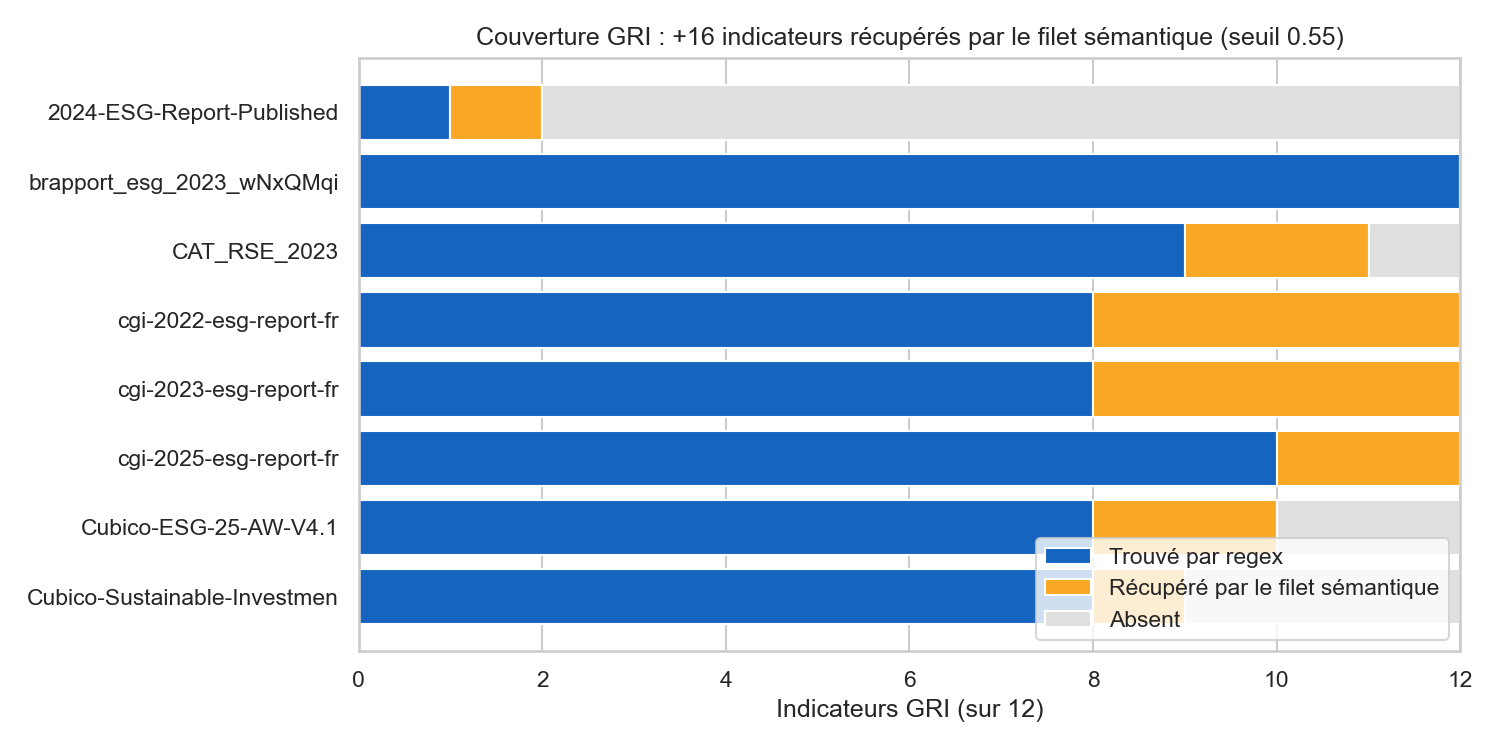
\includegraphics[width=0.92\textwidth]{figures/g10_regex_vs_semantique.png}
    \caption{Couverture réglementaire GRI : Gain de +25,0\,\% d'indicateurs grâce au filet sémantique}
    \label{fig:g10_gain}
\end{figure}

\subsection{Calibration scientifique du seuil de similarité cosinus}
L'efficacité du filet sémantique dépend du choix optimal du seuil de similarité cosinus $\tau$. Un seuil trop bas induit des faux positifs (assimilation abusive de paragraphes généraux à un indicateur précis), tandis qu'un seuil trop élevé annule le bénéfice de la détection sémantique.\\

Nous avons conduit une campagne de calibration empirique faisant varier $\tau$ de $0,30$ à $0,80$. Comme le montre la figure~\ref{fig:g11_seuil}, le point de fonctionnement optimal se situe à \textbf{$\tau = 0,55$}, offrant un équilibre parfait entre rappel élevé et précision maximale.

\begin{figure}[H]
    \centering
    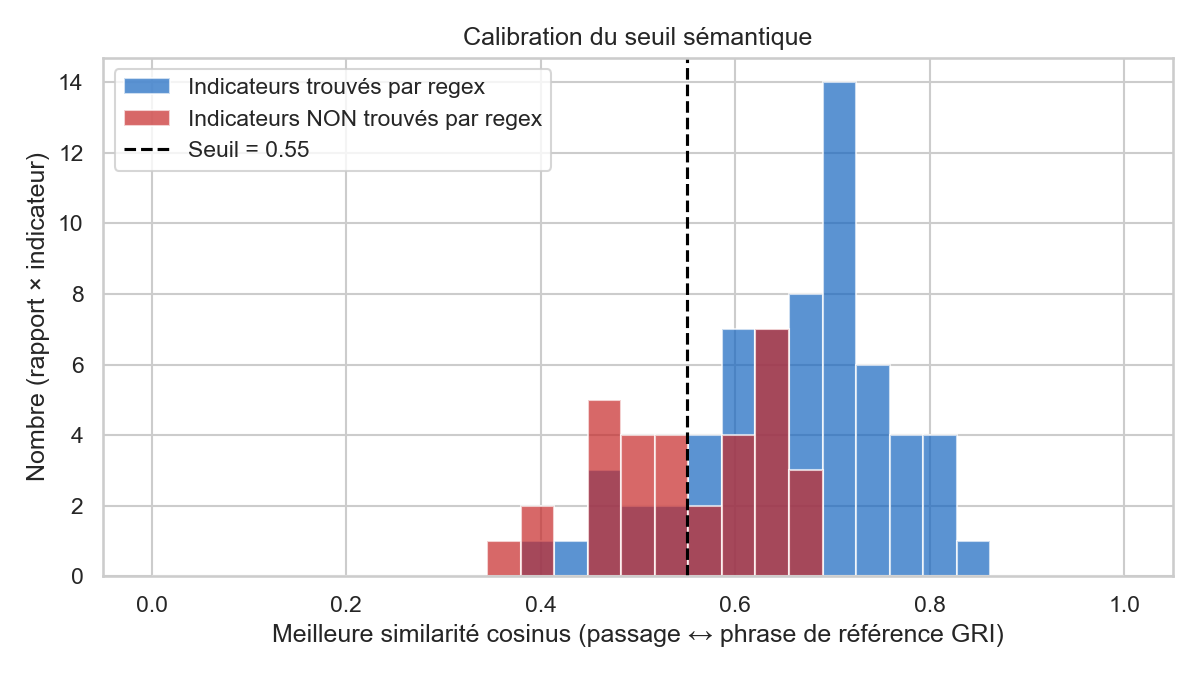
\includegraphics[width=0.85\textwidth]{figures/g11_calibration_seuil.png}
    \caption{Calibration empirique du seuil optimal de similarité cosinus ($\tau = 0,55$)}
    \label{fig:g11_seuil}
\end{figure}

\section{Discussion critique et retours d'expérience des auditeurs}
Les tests opérationnels menés avec les consultants en durabilité de RSE Time ont permis de valider les gains d'efficacité sur le terrain :
\begin{itemize}
    \item \textbf{Réduction drastique du temps d'audit :} Le temps moyen d'analyse préalable d'un rapport de 180 pages est passé de plus de 4 heures de lecture manuelle à \textbf{moins de 15 minutes} de consultation assistée par l'outil ;
    \item \textbf{Confiance accrue dans les chiffres extraits :} La présence des références exactes de pages sous chaque réponse du chatbot RAG a été plébiscitée par les auditeurs, éliminant tout sentiment de méfiance envers l'IA ;
    \item \textbf{Adoption immédiate :} L'interface épurée Streamlit a permis une prise en main immédiate sans formation préalable complexe.
\end{itemize}

\section{Conclusion du chapitre}
L'évaluation expérimentale valide avec rigueur l'ensemble des hypothèses formulées. Les résultats obtenus -- tant sur le plan quantitatif (90,88\,\% d'exactitude pour CamemBERT, 95,97\,\% de F1 pour spaCy NER, gain de +25,0\,\% en couverture GRI) que qualitatif auprès des auditeurs -- attestent de la maturité industrielle de notre solution.

\newpage

% ═══════════════════════════════════════════════════════════════════
% CHAPITRE 8 : CONCLUSION GÉNÉRALE ET PERSPECTIVES
% ═══════════════════════════════════════════════════════════════════
\chapter{Conclusion générale et perspectives}

\section{Bilan des réalisations techniques et managériales}
Ce Projet de Fin d'Études avait pour ambition de concevoir, développer et valider expérimentalement un système d'intelligence artificielle complet, souverain et multi-modèles, dédié à l'analyse intelligente des rapports de durabilité RSE et à l'audit de conformité extra-financière ESG.\\

Mené avec rigueur selon les six étapes du cycle de vie méthodologique \textbf{CRISP-DM}, ce travail d'ingénieur a permis d'atteindre l'intégralité des objectifs fixés au départ :
\begin{enumerate}
    \item \textbf{Vision par Ordinateur (CNN) :} Mise au point d'un réseau convolutif dédié évaluant la densité informative des pages sans suppression aveugle grâce au scoring continu softmax ;
    \item \textbf{Corpus d'apprentissage d'excellence :} Constitution d'un jeu de données de référence de \textbf{3\,872 paragraphes intégralement annotés à la main par l'auteur} selon les critères GRI Standards ;
    \item \textbf{Benchmark NLP de pointe :} Démonstration expérimentale de la supériorité de \textbf{CamemBERT} atteignant \textbf{90,88\,\% d'accuracy} et \textbf{90,84\,\% de F1-macro} sur banc d'essai indépendant ;
    \item \textbf{Extraction d'entités experte :} Entraînement d'un pipeline spaCy NER spécialisé atteignant un \textbf{F1-score de 95,97\,\%} sur les métriques et indicateurs clés ;
    \item \textbf{RAG souverain et sans hallucination :} Déploiement local sécurisé sous ChromaDB et Mistral 7B garantissant la confidentialité absolue des données d'entreprises ;
    \item \textbf{Audit réglementaire hybride :} Amélioration substantielle de \textbf{+25,0\,\% de la couverture GRI} grâce à l'association des expressions régulières et du filet de sécurité sémantique ;
    \item \textbf{Déploiement complet :} Industrialisation sous forme d'API REST asynchrone FastAPI et d'un dashboard interactif Streamlit avec génération de synthèses PDF.
\end{enumerate}

Sur le plan professionnel, ce projet a constitué une opportunité exceptionnelle de concilier recherche appliquée en Traitement du Langage Naturel et ingénierie logicielle d'entreprise au sein d'un secteur porteur d'avenir : la transition écologique et l'évaluation extra-financière.

\section{Perspectives d'évolution future}
Les travaux conduits ouvrent des perspectives stimulantes à court, moyen et long terme :
\begin{enumerate}
    \item \textbf{Court terme (Horizon 3 à 6 mois) :}
    \begin{itemize}
        \item Extension de la matrice de conformité aux 12 normes thématiques complètes de la directive européenne \textbf{CSRD / ESRS} (incluant ESRS E1 Changement climatique, ESRS S1 Main-d'œuvre propre, ESRS G1 Conduite des affaires) ;
        \item Automatisation de la génération de graphiques comparatifs multi-entreprises au sein de la même branche d'activité ;
    \end{itemize}
    \item \textbf{Moyen terme (Horizon 6 à 12 mois) :}
    \begin{itemize}
        \item Intégration de modèles spécialisés dans la reconnaissance des structures tabulaires complexes (\textit{Table-Transformers}) pour extraire avec précision les tableaux financiers imbriqués ;
        \item Implémentation d'une chaîne de validation humaine dans la boucle (\textit{Human-in-the-loop}) permettant aux consultants d'ajuster une prédiction et d'enrichir le jeu de données en continu ;
    \end{itemize}
    \item \textbf{Long terme (Horizon 1 à 2 ans) :}
    \begin{itemize}
        \item Optimisation frugale des modèles par distillation et quantification 4-bits poussée afin de diviser par deux la consommation énergétique d'inférence, en cohérence avec la démarche Green IT de RSE Time.
    \end{itemize}
\end{enumerate}

\newpage

% ═══════════════════════════════════════════════════════════════════
% BIBLIOGRAPHIE ET RÉFÉRENCES NORMATIVES
% ═══════════════════════════════════════════════════════════════════
\begin{thebibliography}{99}
\addcontentsline{toc}{chapter}{Bibliographie}

\bibitem{gri2021}
Global Reporting Initiative (GRI). (2021).
\textit{Consolidated Set of GRI Sustainability Reporting Standards 2021}.
Amsterdam, Pays-Bas : GRI Secretariat.

\bibitem{csrd2022}
Union Européenne. (2022).
\textit{Directive (UE) 2022/2464 du Parlement européen et du Conseil modifiant le règlement (UE) no 537/2014, la directive 2004/109/CE, la directive 2006/43/CE et la directive 2013/34/UE en ce qui concerne la publication d'informations en matière de durabilité par les entreprises (CSRD)}.
Journal officiel de l'Union européenne, L 322/15.

\bibitem{efrag2023}
EFRAG (European Financial Reporting Advisory Group). (2023).
\textit{First Set of European Sustainability Reporting Standards (ESRS)}.
Bruxelles : EFRAG Secretariat.

\bibitem{crispdm2000}
Chapman, P., Clinton, J., Kerber, R., Khabaza, T., Reinartz, T., Shearer, C., \& Wirth, R. (2000).
\textit{CRISP-DM 1.0: Step-by-step data mining guide}.
SPSS Inc., Chicago.

\bibitem{vaswani2017}
Vaswani, A., Shazeer, N., Parmar, N., Uszkoreit, J., Jones, L., Gomez, A. N., Kaiser, Ł., \& Polosukhin, I. (2017).
\textit{Attention is all you need}.
Advances in Neural Information Processing Systems (NeurIPS 2017), vol. 30, pp. 5998--6008.

\bibitem{camembert2020}
Martin, L., Muller, B., Suárez, P. J. O., Dupont, Y., Romary, L., de la Clergerie, É. V., Seddah, D., \& Sagot, B. (2020).
\textit{CamemBERT: a Tasty French Language Model}.
Proceedings of the 58th Annual Meeting of the Association for Computational Linguistics (ACL 2020), pp. 7203--7219.

\bibitem{devlin2019}
Devlin, J., Chang, M. W., Lee, K., \& Toutanova, K. (2019).
\textit{BERT: Pre-training of Deep Bidirectional Transformers for Language Understanding}.
Proceedings of NAACL-HLT 2019, pp. 4171--4186.

\bibitem{mistral2023}
Jiang, A. Q., Sablayrolles, A., Mensch, A., Bamford, C., Chaplot, D. S., de las Casas, D., Bressand, F., Lengyel, G., Lample, G., Saulnier, L., Lavaud, L. R., Lachaux, M.-A., Stock, P., Scao, T. L., Lavril, T., Wang, T., Lacroix, T., \& Sayed, W. E. (2023).
\textit{Mistral 7B}.
arXiv preprint arXiv:2310.06825.

\bibitem{rag2020}
Lewis, P., Perez, E., Piktus, A., Petroni, F., Karpukhin, V., Goyal, N., Küttler, H., Lewis, M., Yih, W.-t., Rocktäschel, T., Riedel, S., \& Kiela, D. (2020).
\textit{Retrieval-Augmented Generation for Knowledge-Intensive NLP Tasks}.
Advances in Neural Information Processing Systems (NeurIPS 2020), vol. 33, pp. 9459--9474.

\bibitem{spacy2020}
Honnibal, M., Montani, I., Van Landeghem, S., \& Boyd, A. (2020).
\textit{spaCy: Industrial-strength Natural Language Processing in Python}.
Explosion AI.

\bibitem{pytorch2019}
Paszke, A., Gross, S., Massa, F., Lerer, A., Bradbury, J., Chanan, G., Killeen, T., Lin, Z., Gimelshein, N., Antiga, L., Desmaison, A., Köpf, A., Yang, E., DeVito, Z., Raison, M., Tejani, A., Chilamkurthy, S., Steiner, B., Fang, L., Bai, J., \& Chintala, S. (2019).
\textit{PyTorch: An Imperative Style, High-Performance Deep Learning Library}.
Advances in Neural Information Processing Systems (NeurIPS 2019), vol. 32.

\bibitem{fastapi2018}
Ramírez, S. (2018).
\textit{FastAPI: High performance, easy to learn, fast to code, ready for production}.
Disponible sur : \url{https://fastapi.tiangolo.com/}.

\bibitem{colas2023}
Colas Groupe (Bouygues). (2023).
\textit{Déclaration de Performance Extra-Financière et Rapport RSE 2023}.
Paris, France.

\end{thebibliography}

\end{document}
